%% ===================================================================
%%  Single inclusive gluon production at NLO at mid rapidity
%%
%%  Compiles with REVTeX 4.2 (aps, prd) when revtex4-2.cls is installed,
%%  and falls back to the standard article class otherwise.
%%
%%  Single-file version generated by flatten.py: all sections and
%%  appendices are inlined. Edit the multi-file sources instead.
%%
%%  Open items of the calculation are typeset with \note{...} (red).
%%  To hide them in a submission version, set \shownotesfalse below.
%%  Source comments marked  %TODO  list the same items.
%% ===================================================================
\newif\ifrevtex
\IfFileExists{revtex4-2.cls}{\revtextrue}{\revtexfalse}
\ifrevtex
  \documentclass[aps,prd,onecolumn,superscriptaddress,nofootinbib,floatfix,longbibliography,11pt]{revtex4-2}
\else
  \documentclass[11pt]{article}
  \usepackage[margin=1in]{geometry}
  \usepackage{titlesec}
  \newcommand{\subseclabel}{\Alph{subsection}}
  \titleformat{\section}{\normalfont\large\bfseries\centering}{\thesection.}{0.6em}{\MakeUppercase}
  \titleformat{\subsection}{\normalfont\normalsize\bfseries\centering}{\subseclabel.}{0.5em}{}
  \titleformat{\subsubsection}{\normalfont\normalsize\itshape}{\arabic{subsubsection}.}{0.5em}{}
  \renewcommand{\thesection}{\Roman{section}}
  \renewcommand{\thesubsection}{\thesection.\Alph{subsection}}
  %% wider number boxes in the table of contents (roman section numbers)
  \usepackage{etoolbox}
  \makeatletter
  \patchcmd{\l@section}{1.5em}{2.4em}{}{}
  \renewcommand*\l@subsection{\@dottedtocline{2}{2.4em}{3.4em}}
  \makeatother
\fi

\usepackage{amsmath,amssymb,amsfonts,bm}
\usepackage{graphicx}
\usepackage[dvipsnames]{xcolor}
\usepackage{booktabs}
\usepackage{array}
\newcolumntype{L}[1]{>{\raggedright\arraybackslash}p{#1}}
\usepackage{tikz}
\usetikzlibrary{arrows.meta,decorations.pathmorphing,decorations.pathreplacing,calc}
\usepackage[colorlinks=true,linkcolor=blue,citecolor=blue,urlcolor=blue]{hyperref}

\allowdisplaybreaks
%% float placement: allow tall tables near their first mention
\renewcommand{\topfraction}{0.9}
\renewcommand{\bottomfraction}{0.8}
\renewcommand{\textfraction}{0.07}
\renewcommand{\floatpagefraction}{0.75}
\setcounter{topnumber}{3}
\setcounter{totalnumber}{4}
\emergencystretch=3em
\numberwithin{equation}{section}
\ifrevtex\else
  \newenvironment{acknowledgments}{\section*{Acknowledgments}}{}
\fi

%% ----- notes for open items ---------------------------------------
\newif\ifshownotes \shownotestrue
\newcommand{\note}[1]{\ifshownotes{\color{red}\,[\textsf{Note:} #1]}\fi}

%% ----- notation ----------------------------------------------------
\newcommand{\kp}{k^{+}}
\newcommand{\pp}{p^{+}}
\newcommand{\qp}{q^{+}}
\newcommand{\V}{\vee}
\newcommand{\dY}{\delta Y}
\newcommand{\dYT}{\delta Y_{T}}
\newcommand{\dYP}{\delta Y_{P}}
\newcommand{\KK}{\mathcal{K}}
\newcommand{\Ud}{U^{\dagger}}
\newcommand{\Tr}{\mathrm{Tr}}
\newcommand{\tr}{\mathrm{tr}}
\def\mf#1{\mathbb{#1}}
\newcommand{\lV}{\ell_{\vee}}
\newcommand{\lL}{\ell_{\Lambda}}
\newcommand{\lLb}{\bar\ell_{\Lambda}}
\newcommand{\Lp}{\mathcal{L}_{+}}
\newcommand{\Lo}{\mathcal{L}_{1}}
\newcommand{\Lop}{\mathcal{L}_{1}'}
\newcommand{\Lt}{\mathcal{L}_{2}}
\newcommand{\Lf}{\mathcal{L}_{4}}
\newcommand{\Phat}{\hat P}
\newcommand{\pre}{\frac{1}{(2\pi)^3}\int_{w,w'}e^{-ik\cdot(w'-w)}}
\newcommand{\ket}[1]{\left|#1\right\rangle}
\newcommand{\bra}[1]{\left\langle #1\right|}
\newcommand{\Ord}{\mathcal{O}}
\newcommand{\MSbar}{\overline{\rm MS}}
\newcommand{\eps}{\epsilon}

\begin{document}

\title{Single inclusive gluon production at next-to-leading order at mid rapidity}

\ifrevtex
  %% Author names and affiliations are placeholders.
  \author{[Author 1]}
  \affiliation{[Affiliation 1]}
  \author{[Author 2]}
  \affiliation{[Affiliation 2]}
  \date{\today}
\else
  \author{[Author 1]$^{1}$ \ and \ [Author 2]$^{2}$\\[4pt]
  {\small\itshape $^{1}$[Affiliation 1]}\\
  {\small\itshape $^{2}$[Affiliation 2]}}
  \date{\today}
\fi

\newcommand{\abstracttext}{%
We compute the single inclusive gluon production cross section in the scattering of a dilute projectile on a dense target at next-to-leading order, i.e.\ at order $g^4$ relative to the order-$g^2$ leading result, in the light-cone wave function approach. The soft gluon Fock space of the projectile, $\Lambda<k^+<\vee$, is dressed by a unitary evolution operator $\Omega$. Its coefficients are fixed to order $g^3$ by matching to the light-cone perturbation theory wave functions of the valence vacuum and of a single-gluon state. The cross section is organized into virtual (one gluon in the final state), real (two gluons) and interference contributions, which we evaluate in transverse coordinate space. At leading logarithmic accuracy the rapidity interval $\delta Y=\log(\vee/\Lambda)$ opened by the unobserved gluon is shared. The part above the measured gluon, $\log(\vee/k^+)$, evolves the projectile charge correlator with the BFKL equation. The part below it, $\log(k^+/\Lambda)$, evolves the target Wilson lines with the JIMWLK Hamiltonian, whose action is obtained as a double commutator of the soft-gluon emission operators. All terms with three and four valence charges cancel. We define the next-to-leading-order remainder by an exact subtraction of the two logarithms and give it term by term. All power-like terms $\propto 1/\Lambda$ cancel once the relative sign of the two orderings in the one-gluon wave function is fixed by the endpoint behaviour at $p^+\to k^+$. The real gluon splitting function appears in the self-energy of the emitted gluon, in the loop across the target and in the initial-state, interference and final-state collinear splittings. We use this to separate the $\beta_0$ terms associated with the running of the coupling from those associated with DGLAP evolution of the projectile and with fragmentation.}

\ifrevtex
  \begin{abstract}\abstracttext\end{abstract}
  \maketitle
\else
  \maketitle
  \begin{abstract}\abstracttext\end{abstract}
\fi

\tableofcontents

%% >>> begin sec1_intro.tex
%% ===================================================================
\section{Introduction}\label{sec:intro}
%% ===================================================================

Inclusive production of a single gluon in the collision of a dilute projectile with a dense target is the simplest observable that probes the nonlinear regime of QCD at high energy. In the colour glass condensate (CGC) effective theory~\cite{McLerran:1993ni,McLerran:1993ka} the target is described by eikonal Wilson lines $U(x)$ in the adjoint representation, and the projectile by the colour charge density $\rho^a(x)$ of its fast (valence) partons together with the cloud of soft gluons that these charges radiate. At leading order (LO) in the strong coupling the gluon spectrum is known in closed form~\cite{Kovchegov:1998bi,Kovchegov:2001sc,Dumitru:2001ux,Blaizot:2004wu,Kovner:2006wr}. The measured gluon is emitted by a valence charge either before or after the eikonal interaction with the target. The cross section is a convolution of the projectile charge correlator $\langle\rho\rho\rangle$ with a target correlator of the form $\Tr\{[\Ud(x)-\Ud(w)][U(x')-U(w')]\}$.

At high energy these correlators are dressed by large logarithms of the energy. At leading-logarithmic (LL) accuracy the produced gluon at rapidity $y$ divides the evolution into two parts~\cite{Kovchegov:2001sc,Baier:2005dv,Kovner:2006ge,Kovner:2006wr,Gelis:2008rw}. The projectile is evolved from its own rapidity down to $y$ and the target from its rapidity up to $y$. In the dilute projectile the charge correlator then obeys the BFKL equation~\cite{Kuraev:1977fs,Balitsky:1978ic}. The target Wilson lines obey the JIMWLK equation~\cite{JalilianMarian:1997jx,JalilianMarian:1997gr,JalilianMarian:1998cb,Kovner:2000pt,Weigert:2000gi,Iancu:2000hn,Ferreiro:2001qy}, whose large-$N_c$ mean-field limit is the Balitsky--Kovchegov (BK) equation~\cite{Balitsky:1995ub,Kovchegov:1999yj}.

At next-to-leading order (NLO) much less is known about this observable. The evolution equations themselves are available at NLO: the NLO BK equation~\cite{Balitsky:2007feb} and the NLO JIMWLK Hamiltonian~\cite{Balitsky:2013fea,Kovner:2013ona,Kovner:2014lca,Lublinsky:2016meo}, together with their running-coupling content~\cite{Balitsky:2006wa,Kovchegov:2006vj}. Running-coupling corrections to the LO gluon spectrum were obtained in Ref.~\cite{Horowitz:2010yg}. Recently it was shown that some of the $\beta_0$-dependent transverse logarithms of NLO JIMWLK are not related to the running of the coupling. They are instead the first step of DGLAP evolution of the projectile~\cite{Kovner:2023vsy,Altinoluk:2023hfz}. Complete NLO results exist for single inclusive \emph{hadron} production at forward rapidity in the hybrid formalism~\cite{Chirilli:2011km,Chirilli:2012jd,Stasto:2013cha,Altinoluk:2014eka,Ducloue:2016shw,Iancu:2016vyg}. There the projectile is described by collinear parton distributions, and only the target undergoes small-$x$ evolution. These studies showed that the subtraction of the rapidity divergence, and the precise rapidity interval assigned to the evolution, are delicate at NLO.

At mid rapidity both the projectile and the target are probed at small $x$, and both must be treated in the same framework. In this paper we compute the single inclusive gluon spectrum at NLO, i.e.\ to order $g^4$, in the light-cone wave function (LCWF) approach~\cite{Lepage:1980fj,Brodsky:1997de,Kovner:2005nq,Kovner:2013ona,Kovner:2014lca,Lublinsky:2016meo}. The soft gluon modes of the projectile, with longitudinal momenta $\Lambda<k^+<\vee$, are dressed by a unitary operator $\Omega$ that acts on the valence state. The coefficients of $\Omega$ are fixed to order $g^3$ by light-cone perturbation theory (LCPT). The cross section is then the expectation value of the number operator of \emph{dressed} gluons in the scattered state. This construction treats real and virtual corrections, and initial- and final-state radiation, on the same footing.

Our main results are the following.
\begin{enumerate}
\item We give the NLO LCWF of the valence vacuum to order $g^3$ and of a single-gluon state to order $g^2$ in transverse coordinate space. We use them to fix the coefficients $\mf N$, $\mf A^{(1)}$, $\mf A^{(3)}$, $\mf B_2$, $\mf B_3$ and $\mf C_1$ of $\Omega$; the remaining coefficients follow from unitarity (Secs.~\ref{sec:lcwf} and~\ref{sec:omega}). The one-gluon wave function has two orderings, with the outgoing soft gluon harder or softer than the incoming one. The relative sign of their non-instantaneous parts is fixed by requiring that the double pole $1/(p^+-k^+)^2$ of the instantaneous interaction cancels on both sides of $p^+=k^+$.
\item We write the NLO cross section as a sum of products of these coefficients. There are five classes of virtual (one-gluon) terms, four classes of squared real (two-gluon) amplitudes and six classes of interference terms (Sec.~\ref{sec:xsec}).
\item At LL accuracy the full rapidity interval $\delta Y=\log(\vee/\Lambda)$ opened by the unobserved gluon is shared between the projectile and the target (Sec.~\ref{sec:LL}):
\begin{equation}
\frac{d^3N}{d^3k}\bigg|_{\rm LL}=\log\frac{\vee}{k^+}\,\big[{\rm BFKL}\otimes{\rm LO}\big]+\log\frac{k^+}{\Lambda}\,\big[{\rm JIMWLK}\otimes{\rm LO}\big].
\label{eq:intro-main}
\end{equation}
Real and virtual terms combine into a double commutator of soft-gluon emission operators. Its action on the LO cross section is exactly that of the JIMWLK Hamiltonian, including the terms in which the soft gluon is emitted by the measured gluon itself. All contributions with three or four valence charges cancel.
\item We define the NLO remainder (the ``finite part'') by an exact subtraction of $\log(k^+/\Lambda)$ and $\log(\vee/k^+)$, keeping all dependence on the finite upper cutoff $\vee$. We give this remainder term by term and show that all power-like terms $\propto1/\Lambda$ cancel (Sec.~\ref{sec:finite}).
\item The real gluon splitting function appears in four places: in the self-energy of the emitted gluon, in the loop across the target, and in the initial-state, interference and final-state collinear splittings. The real collinear terms come with relative weights $1:-2:1$. We use this to separate the $\beta_0$ terms associated with the running coupling from those associated with DGLAP evolution of the projectile and with fragmentation, along the lines of Ref.~\cite{Kovner:2023vsy} (Sec.~\ref{sec:rc}).
\end{enumerate}

The paper is organized as follows. Section~\ref{sec:framework} sets up the light-cone Hamiltonian, the evolution operator $\Omega$, the scattering and the cross section, and recalls the LO result. Section~\ref{sec:lcwf} collects the LCWFs, and Sec.~\ref{sec:omega} the resulting coefficients of $\Omega$. Section~\ref{sec:xsec} gives the cross section at order $g^4$. The leading logarithms are extracted in Sec.~\ref{sec:LL}, the finite part in Sec.~\ref{sec:finite}, and the running coupling and DGLAP terms are discussed in Sec.~\ref{sec:rc}. We summarize in Sec.~\ref{sec:summary}. The appendices contain conventions, matrix elements and Fourier transforms (App.~\ref{app:conv}), the longitudinal integrals (App.~\ref{app:long}), the explicit form of JIMWLK$\otimes$LO and BFKL$\otimes$LO (App.~\ref{app:explicit}), the LL content of every term of the cross section (App.~\ref{app:LLrows}), and the numerical checks (App.~\ref{app:checks}).
%% <<< end sec1_intro.tex
%% >>> begin sec2_framework.tex
%% ===================================================================
\section{Framework}\label{sec:framework}
%% ===================================================================

\subsection{Soft gluons, valence charges and the light-cone Hamiltonian}\label{sec:hamiltonian}

We work in light-cone gauge $A^+=0$ with the projectile moving in the $+$ direction. The gluon field is split into soft modes, with longitudinal momenta in the window $\Lambda<k^+<\vee$, and faster (valence) modes with $k^+>\vee$~\cite{Kovner:2005nq,Lublinsky:2016meo}:
\begin{equation}
A_i^a(x)=\int_{\Lambda}^{\vee}\frac{dk^+}{2\pi}\int\frac{d^2\mathbf k}{(2\pi)^2}\frac{1}{\sqrt{2k^+}}\Big(a_i^a(k^+,\mathbf k)\,e^{-ik\cdot x}+a_i^{a\dagger}(k^+,\mathbf k)\,e^{ik\cdot x}\Big)+\big(\text{modes with }k^+>\vee\big).
\label{eq:Asoft}
\end{equation}
In the eikonal (CGC) approximation the valence modes enter only through their colour charge density $\rho^a(x)$, a function of the transverse position $x$. Its components obey the $SU(N_c)$ algebra
\begin{equation}
[\rho^a(x),\rho^b(y)]=if^{abc}\rho^c(x)\,\delta^{(2)}(x-y).
\label{eq:rhoalg}
\end{equation}
The soft creation and annihilation operators satisfy $[a^a_i(k),a^{b\dagger}_j(p)]=(2\pi)^3\delta^{ab}\delta_{ij}\delta^{(3)}(k-p)$, with $\delta^{(3)}(k-p)=\delta(k^+-p^+)\delta^{(2)}(\mathbf k-\mathbf p)$. Throughout, $x,y,z,u,v,w,\ldots$ denote two-dimensional transverse positions, $\int_x\equiv\int d^2x$, and the transverse Fourier conventions are
\begin{equation}
a(k^+,\mathbf k)=\int d^2z\,e^{-i\mathbf k\cdot z}a(k^+,z),\qquad a^\dagger(k^+,\mathbf k)=\int d^2z\,e^{i\mathbf k\cdot z}a^\dagger(k^+,z),\qquad f(\mathbf k)=\int d^2x\,e^{i\mathbf k\cdot x}f(x),
\label{eq:FTconv}
\end{equation}
so that $[a^a_i(k^+,z),a^{b\dagger}_j(p^+,z')]=2\pi\,\delta^{ab}\delta_{ij}\delta(k^+-p^+)\delta^{(2)}(z-z')$.

The light-cone Hamiltonian is $H=H_0+H_{\rm int}$. The free part gives a soft gluon the energy $E_g(k)=\mathbf k^2/2k^+$. The interaction terms that contribute at the order we work are~\cite{Lublinsky:2016meo}:
\begin{itemize}
\item $H_g$, the emission and absorption of a soft gluon by the valence charges,
\begin{equation}
H_g=\int_{\Lambda}^{\vee}\frac{dk^+}{2\pi}\int\frac{d^2\mathbf k}{(2\pi)^2}\,\frac{g\,\mathbf k^i}{\sqrt2\,|k^+|^{3/2}}\Big[a_i^{a\dagger}(k^+,\mathbf k)\,\rho^a(-\mathbf k)+a_i^a(k^+,\mathbf k)\,\rho^a(\mathbf k)\Big];
\label{eq:Hg}
\end{equation}
\item $H_{ggg}$, the three-gluon vertex among soft gluons;
\item $H_{gg\text{-inst}}$, the instantaneous interaction of two soft gluons with the valence charge (from the longitudinal Coulomb field in light-cone gauge).
\end{itemize}
Their matrix elements between Fock states are collected in App.~\ref{app:conv}, Eqs.~\eqref{eq:m1}--\eqref{eq:m5}. The quartic soft vertex and quark loops are not needed for gluon production at this order, except through the gluon self-energy, where we keep only the gluon loop ($n_f=0$).

\subsection{The dressed projectile and the evolution operator \texorpdfstring{$\Omega$}{Omega}}\label{sec:Omega}

Let $|0\rangle$ be the state with the valence charges and no soft gluons. The physical projectile is the eigenstate of $H$ that reduces to $|0\rangle$ at $g=0$. Light-cone perturbation theory~\cite{Lepage:1980fj,Brodsky:1997de} constructs it order by order:
\begin{equation}
|\Psi\rangle=\mf N|0\rangle+\sum_n|n\rangle\frac{\langle n|H_{\rm int}|0\rangle}{E_0-E_n}+\sum_{n,m}|n\rangle\frac{\langle n|H_{\rm int}|m\rangle\langle m|H_{\rm int}|0\rangle}{(E_0-E_n)(E_0-E_m)}+\dots,\qquad E_0=0,
\label{eq:LCPT}
\end{equation}
where $|n\rangle,|m\rangle$ are free Fock states of soft gluons and $\mf N$ is fixed by normalization. The same construction dresses any soft state, e.g.\ a single soft gluon $|g^a_i(k)\rangle$. We write all dressed states with one unitary operator $\Omega$,
\begin{equation}
|\Psi\rangle=\Omega|0\rangle,\qquad |\Psi^a_i(k)\rangle=\Omega\,|g^a_i(k)\rangle,\qquad \Omega^\dagger\Omega=1.
\label{eq:Omegadef}
\end{equation}
$\Omega$ acts on the soft Fock space and depends on the valence charges $\rho$. Normal ordering the soft operators gives~\cite{Lublinsky:2016meo}
\begin{align}
\Omega={}&\mf N+\int\frac{d^3p}{(2\pi)^3}\Big[\mf A^b_{1j}(p)\,a^b_j(p)+\mf A^b_{2j}(p)\,a^{b\dagger}_j(p)\Big]\notag\\
&+\int\frac{d^3p}{(2\pi)^3}\frac{d^3q}{(2\pi)^3}\Big[\mf B^{cb}_{1kj}(p,q)\,a^b_j(p)a^c_k(q)+\mf B^{cb}_{2kj}(p,q)\,a^{b\dagger}_j(p)a^{c\dagger}_k(q)+\mf B^{cb}_{3kj}(p,q)\,a^{c\dagger}_k(q)a^b_j(p)\Big]\notag\\
&+\int\frac{d^3p}{(2\pi)^3}\frac{d^3q}{(2\pi)^3}\Big[\mf C^{dcb}_{1lkj}(p,q)\,a^{d\dagger}_l(q)a^{c\dagger}_k(p-q)a^b_j(p)+\mf C^{dcb}_{2lkj}(p,q)\,a^{b\dagger}_j(p)a^c_k(p-q)a^d_l(q)\Big]+\dots
\label{eq:OmegaExp}
\end{align}
The coefficients are operators in the valence colour space. Bose symmetry implies $\mf B^{cb}_{1kj}(p,q)=\mf B^{bc}_{1jk}(q,p)$, $\mf B^{cb}_{2kj}(p,q)=\mf B^{bc}_{2jk}(q,p)$ and $\mf C^{dcb}_{1lkj}(p,q)=\mf C^{cdb}_{1klj}(p,p-q)$ (and the same for $\mf C_2$). The dots stand for terms with more soft operators, which do not contribute to single gluon production at order $g^4$. The coefficients mix orders in $g$. We need $\mf N=1+\mf N_2$ to order $g^2$ and
\begin{equation}
\mf A_{1,2}=\mf A^{(1)}_{1,2}+\mf A^{(3)}_{1,2}
\end{equation}
to order $g^3$. $\mf B_{1,2,3}$ are needed at order $g^2$ and $\mf C_{1,2}$ at order $g$.

\paragraph*{Unitarity.} The condition $\Omega^\dagger\Omega=1$, normal ordered, relates the daggered and undaggered coefficients. To the order needed, and with $\mf N=\mf N^\dagger$,
\begin{align}
&\mf N=1-\frac12\int\frac{d^3p}{(2\pi)^3}\,\mf A^{b}_{1j}(p)\,\mf A^{\dagger b}_{1j}(p),\label{eq:unitN}\\
&\mf A^{(1)\dagger b}_{1j}(p)=-\mf A^{(1)b}_{2j}(p),\label{eq:unitA1}\\
&\mf A^{(3)\dagger b}_{1j}(p)=-\mf A^{(3)b}_{2j}(p)-\big[\mf N_2,\mf A^{(1)b}_{2j}(p)\big]+\int\frac{d^3q}{(2\pi)^3}\Big[2\,\mf A^{(1)c}_{1k}(q)\,\mf B^{cb}_{2kj}(p,q)-\mf B^{\dagger cb}_{3kj}(p,q)\,\mf A^{(1)c}_{2k}(q)\notag\\
&\hspace{20em}-2\,\mf C^{\dagger dcb}_{1lkj}(p,q)\,\mf B^{cd}_{2kl}(q,p-q)\Big],\label{eq:unitA3}\\
&\mf B^{\dagger cb}_{1kj}(p,q)=\frac12\Big[-2\,\mf B^{cb}_{2kj}(p,q)+\mf A^{(1)b}_{2j}(p)\,\mf A^{(1)c}_{2k}(q)+\mf A^{(1)c}_{2k}(q)\,\mf A^{(1)b}_{2j}(p)+2\,\mf C^{cbd}_{1kjl}(q+p,q)\,\mf A^{(1)d}_{2l}(q+p)\Big],\label{eq:unitB1}\\
&\mf C^{\dagger dcb}_{2lkj}(p,q)=-\mf C^{dcb}_{1lkj}(p,q).\label{eq:unitC2}
\end{align}
The commutator in Eq.~\eqref{eq:unitA3} does not vanish. $\mf N_2\propto\int K\,\rho^a\rho^a$ [Eq.~\eqref{eq:NX} below] commutes with the total charge $\int_x\rho^a(x)$, but not with the local charge $\rho^b(u)$ in $\mf A^{(1)}$:
\begin{equation}
\Big[\int_{x,y}K(x,y)\,\rho^a(x)\rho^a(y),\ \rho^b(u)\Big]=if^{abc}\int_xK(x,u)\,\big\{\rho^a(x),\rho^c(u)\big\}
\label{eq:Ncomm}
\end{equation}
for a symmetric kernel $K(x,y)=K(y,x)$. It is a two-charge term proportional to $\log(\vee/\Lambda)$ [the logarithm of $\mf N_2$], and therefore contributes only to the leading-logarithmic part of the cross section, never to the finite part of Sec.~\ref{sec:finite}. In Sec.~\ref{sec:LL} the LL part is derived directly from the leading-log form of $\Omega$, in which all such orderings are automatically included.
\note{The draft notes set $[\mf N_2,\mf A^{(1)}]=0$; with Eq.~\eqref{eq:Ncomm} the Group~I bookkeeping of the $\log(\vee/\Lambda)$ terms has to include this commutator.}
%TODO: propagate [N_2, A^(1)] into the row-by-row LL bookkeeping of Group I (4rho notes).
The coefficients $\mf A^{(1)}_1$, $\mf A^{(3)}_2$, $\mf B_2$, $\mf B_3$ and $\mf C_1$ are obtained from LCPT; $\mf A^{(3)}_1$, $\mf B_1$ and $\mf C_2$ then follow from Eqs.~\eqref{eq:unitA3}--\eqref{eq:unitC2}. The product $\mf A^{(1)}\mf A^{(1)}$ in Eq.~\eqref{eq:unitB1} is kept as an operator product: its two orderings differ by the commutator~\eqref{eq:rhoalg}, which is of the same order as the $\rho$-linear part of $\mf B_2$.

\paragraph*{Coordinate space.} With the conventions~\eqref{eq:FTconv}, the expansion~\eqref{eq:OmegaExp} becomes
\begin{align}
\Omega={}&\mf N+\int\frac{dp^+}{2\pi}\int_x\Big[\mf A^{(1)b}_{1j}(p^+,x)\,a^b_j(p^+,x)-\mf A^{\dagger(1)b}_{1j}(p^+,x)\,a^{\dagger b}_j(p^+,x)\notag\\
&\hspace{7em}+\mf A^{(3)b}_{1j}(p^+,x)\,a^b_j(p^+,x)+\mf A^{(3)b}_{2j}(p^+,-x)\,a^{\dagger b}_j(p^+,x)\Big]\notag\\
&+\int\frac{dp^+}{2\pi}\frac{dq^+}{2\pi}\int_{x,y}\Big[\mf B^{cb}_{1kj}(p^+,x;q^+,y)\,a^b_j(p^+,x)a^c_k(q^+,y)\notag\\
&\hspace{7em}+\mf B^{cb}_{2kj}(p^+,-x;q^+,-y)\,a^{\dagger b}_j(p^+,x)a^{\dagger c}_k(q^+,y)\notag\\
&\hspace{7em}+\mf B^{cb}_{3kj}(p^+,x;q^+,-y)\,a^{\dagger c}_k(q^+,y)a^b_j(p^+,x)\Big]\notag\\
&+\int\frac{dp^+}{2\pi}\frac{dq^+}{2\pi}\int_{x,y,z}\Big[\mf C^{dcb}_{1lkj}(p^+,z-y;q^+,y-x)\,a^{\dagger d}_l(q^+,x)a^{\dagger c}_k(p^+-q^+,y)a^b_j(p^+,z)\notag\\
&\hspace{7em}-\mf C^{\dagger dcb}_{1lkj}(p^+,z-y;q^+,y-x)\,a^{\dagger b}_j(p^+,z)a^c_k(p^+-q^+,y)a^d_l(q^+,x)\Big]+\dots,
\label{eq:OmegaX}
\end{align}
where we have used Eqs.~\eqref{eq:unitA1} and~\eqref{eq:unitC2}. The unitarity relations in coordinate space read
\begin{align}
\mf A^{(1)\dagger b}_{1j}(p^+,z)={}&-\mf A^{(1)b}_{2j}(p^+,-z),\label{eq:unitA1X}\\
\mf A^{(3)\dagger b}_{1j}(p^+,x)={}&-\mf A^{(3)b}_{2j}(p^+,-x)-\big[\mf N_2,\mf A^{(1)b}_{2j}(p^+,-x)\big]\notag\\
&+\int\frac{dq^+}{2\pi}\int_y\Big[2\,\mf A^{(1)c}_{1k}(q^+,y)\,\mf B^{cb}_{2kj}(p^+,-x;q^+,-y)\notag\\
&\hspace{5em}-\mf B^{\dagger cb}_{3kj}(p^+,x;q^+,-y)\,\mf A^{(1)c}_{2k}(q^+,-y)\notag\\
&\hspace{5em}-2\int_z\mf C^{\dagger dcb}_{1lkj}(p^+,x-z;q^+,z-y)\,\mf B^{dc}_{2lk}(p^+-q^+,-z;q^+,-y)\Big],\label{eq:unitA3X}\\
\mf B^{\dagger cb}_{1kj}(p^+,x;q^+,y)={}&\frac12\Big[-2\,\mf B^{cb}_{2kj}(p^+,-x;q^+,-y)+\mf A^{(1)b}_{2j}(p^+,-x)\,\mf A^{(1)c}_{2k}(q^+,-y)\notag\\
&\hspace{3em}+\mf A^{(1)c}_{2k}(q^+,-y)\,\mf A^{(1)b}_{2j}(p^+,-x)\notag\\
&\hspace{3em}+2\int_z\mf C^{cbd}_{1kjl}(q^++p^+,z-x;q^+,x-y)\,\mf A^{(1)d}_{2l}(q^++p^+,-z)\Big],\label{eq:unitB1X}\\
\mf C^{\dagger dcb}_{2lkj}(p^+,z;q^+,x)={}&-\mf C^{dcb}_{1lkj}(p^+,-z;q^+,-x).\label{eq:unitC2X}
\end{align}

\paragraph*{Action of $\Omega$ on the vacuum and on one gluon.} The coefficients are read off from
\begin{align}
\Omega|0\rangle={}&\mf N|0\rangle+\frac{1}{(2\pi)^{1/2}}\int dp^+\int_x\Big[\mf A^{(3)b}_{2j}(p^+,-x)-\mf A^{\dagger(1)b}_{1j}(p^+,x)\Big]|g^b_j(p^+,x)\rangle\notag\\
&+\frac{1}{2\pi}\int dp^+dq^+\int_{z,x}\mf B^{cb}_{2kj}(p^+,-z;q^+,-x)\,|g^b_j(p^+,z)\,g^c_k(q^+,x)\rangle,\label{eq:Omegavac}\\[3pt]
\Omega|g^a_i(k^+,z)\rangle={}&\frac{1}{(2\pi)^{1/2}}\Big[\mf A^{(1)a}_{1i}(k^+,z)+\mf A^{(3)a}_{1i}(k^+,z)\Big]|0\rangle+\mf N|g^a_i(k^+,z)\rangle\notag\\
&+\frac{1}{2\pi}\int dp^+\int_x\mf B^{ba}_{3ji}(k^+,z;p^+,-x)\,|g^b_j(p^+,x)\rangle\notag\\
&+\frac{1}{(2\pi)^{1/2}}\int dp^+\int_x\Big[\mf A^{(3)b}_{2j}(p^+,-x)-\mf A^{\dagger(1)b}_{1j}(p^+,x)\Big]|g^a_i(k^+,z)\,g^b_j(p^+,x)\rangle\notag\\
&+\frac{1}{(2\pi)^{1/2}}\int dp^+\int_{x,y}\mf C^{bca}_{1jki}(k^+,z-y;p^+,y-x)\,|g^b_j(p^+,x)\,g^c_k(k^+-p^+,y)\rangle+\dots,\label{eq:Omegag}
\end{align}
with the states of App.~\ref{app:conv}. Comparing Eq.~\eqref{eq:Omegavac} with the LCPT vacuum wave function fixes $\mf N$, $\mf A^{(1)}$, $\mf A^{(3)}_2$ and $\mf B_2$. Comparing Eq.~\eqref{eq:Omegag} with the dressed one-gluon state fixes $\mf B_3$ and $\mf C_1$.

\subsection{Scattering and the inclusive cross section}\label{sec:xsecdef}

The target acts on the projectile through the eikonal $S$-matrix. Every colour charge, valence or soft, is rotated by the adjoint Wilson line of the target at its transverse position~\cite{Kovner:2005nq}:
\begin{equation}
S^\dagger\rho^a(x)S=U^{ab}(x)\rho^b(x),\quad S^\dagger a^a_i(k^+,x)S=U^{ab}(x)\,a^b_i(k^+,x),\quad S^\dagger a^{a\dagger}_i(k^+,x)S=U^{ab}(x)\,a^{b\dagger}_i(k^+,x).
\label{eq:Srot}
\end{equation}
Here $U(x)=\mathcal P\exp\{ig\int dx^+T^a\alpha^a(x^+,x)\}$, with $(T^a)_{bc}=-if^{abc}$ and $\alpha^a$ the target field. $U$ is real and orthogonal, $U^\dagger=U^T$. We denote a rotated operator by a bar, e.g.\ $\bar\Omega\equiv S^\dagger\Omega S$, which is $\Omega$ with $\rho\to U\rho$. Rotated coefficients are written $\bar{\mf A}$, $\bar{\mf B}$, $\bar{\mf C}$; for instance $\bar{\mf A}^{(1)}$ is $\mf A^{(1)}$ with $\rho^b(x)\to U^{bc}(x)\rho^c(x)$.

The incoming state is $\Omega|0\rangle$ and the outgoing state is $S\Omega|0\rangle$. The observable is the number of \emph{dressed} gluons in the outgoing state. The number operator of dressed gluons is $\Omega\,a^\dagger a\,\Omega^\dagger$, so
\begin{equation}
\frac{d^3N}{d^3k}=\frac{1}{(2\pi)^3}\int_{w,w'}e^{-ik\cdot(w'-w)}\,\langle0|\,\Omega^\dagger S^\dagger\Omega\;a^{a\dagger}_i(k^+,w)\,a^a_i(k^+,w')\;\Omega^\dagger S\,\Omega\,|0\rangle,
\label{eq:xsec}
\end{equation}
where $d^3k\equiv dk^+d^2\mathbf k$ and the expectation value includes the average over the valence charges and over the target fields. Inserting $SS^\dagger=1$ and complete sets of one- and two-gluon states gives
\begin{equation}
\frac{d^3N}{d^3k}=\frac{1}{(2\pi)^3}\bigg[\underbrace{\mathcal A^{\dagger a}_i(k)\,\mathcal A^a_i(k)}_{\text{one gluon}}+\int dq^+\int_v\underbrace{\mathcal A^{\dagger ab}_{ij}(k;q^+,v)\,\mathcal A^{ab}_{ij}(k;q^+,v)}_{\text{two gluons}}\bigg],
\label{eq:groups}
\end{equation}
with the amplitudes
\begin{align}
\mathcal A^a_i(k)&=\sqrt{2\pi}\int_{w'}e^{-ik\cdot w'}\,U^{ab}(w')\,\langle g^b_i(k^+,w')|\,\bar\Omega^\dagger\Omega\,|0\rangle,\label{eq:amp1}\\
\mathcal A^{ab}_{ij}(k;q^+,v)&=\sqrt{2\pi}\int_{w'}e^{-ik\cdot w'}\,U^{ac}(w')\,\langle g^b_j(q^+,v)\,g^c_i(k^+,w')|\,\bar\Omega^\dagger\Omega\,|0\rangle.\label{eq:amp2}
\end{align}
The operator $\bar\Omega^\dagger\Omega$ makes the structure of Eq.~\eqref{eq:xsec} transparent. $\Omega$ creates the soft cloud of the incoming projectile. The target rotates it, and $\bar\Omega^\dagger=S^\dagger\Omega^\dagger S$ removes the cloud that the \emph{rotated} valence charges carry in the final state. If the target is trivial, $U=1$, then $\bar\Omega^\dagger\Omega=1$ and nothing is produced. The second gluon in Eq.~\eqref{eq:amp2} is unobserved and is integrated over its momentum fraction $q^+$ and position $v$.

\subsection{Leading order}\label{sec:LO}

At order $g$ only $\mf A^{(1)}$ contributes. Using Eq.~\eqref{eq:unitA1X} and the coefficient~\eqref{eq:A1X} below,
\begin{align}
\mathcal A^a_i(k)&=\int_{w'}e^{-ik\cdot w'}\Big[-U^{ab}(w')\,\mf A^{\dagger(1)b}_{1i}(k^+,w')+\bar{\mf A}^{\dagger(1)a}_{1i}(k^+,w')\Big]\notag\\
&=\frac{ig}{\sqrt2\,\pi\sqrt{k^+}}\int_{w'}e^{-ik\cdot w'}\int_x\KK^i(x-w')\big[U(w')-U(x)\big]^{ab}\rho^b(x),
\label{eq:ampLO}
\end{align}
where we introduced the Weizs\"acker--Williams field
\begin{equation}
\KK^i(X)\equiv\frac{X^i}{X^2}.
\end{equation}
The two terms are the emission of the gluon before the target (rotated at $w'$) and after it (the emitter rotated at $x$). The LO spectrum is
\begin{align}
\frac{d^3N_{\rm LO}}{d^3k}={}&\frac{1}{(2\pi)^3}\,\frac{g^2}{2\pi^2k^+}\int_{w,w'}e^{-ik\cdot(w'-w)}\int_{x,x'}\KK(x-w)\cdot\KK(x'-w')\notag\\
&\times\Big\langle\rho^b(x)\Big[\big(\Ud(x)-\Ud(w)\big)\big(U(x')-U(w')\big)\Big]^{bb'}\rho^{b'}(x')\Big\rangle.
\label{eq:LOop}
\end{align}
For a projectile whose colour correlator is diagonal, $\langle\rho^b(x)\rho^{b'}(x')\rangle=\delta^{bb'}\langle\rho^f(x)\rho^f(x')\rangle/(N_c^2-1)$, this becomes the familiar form~\cite{Kovchegov:2001sc,Dumitru:2001ux,Blaizot:2004wu}
\begin{align}
\frac{d^3N_{\rm LO}}{d^3k}={}&\frac{\alpha_s}{4\pi^4(N_c^2-1)\,k^+}\int_{x,w,x',w'}e^{-ik\cdot(w'-w)}\,\KK(x-w)\cdot\KK(x'-w')\notag\\
&\times\langle\rho^f(x)\rho^f(x')\rangle\,\Tr\Big\{\big[\Ud(x)-\Ud(w)\big]\big[U(x')-U(w')\big]\Big\}.
\label{eq:LO}
\end{align}
Integrating over $\mathbf k$ sets $w=w'$ and gives $dN_{\rm LO}/dk^+=(\alpha_s/\pi^2)(1/k^+)\int_w\langle\dots\rangle$. Each additional emission of a gluon with momentum fraction $dq^+/q^+$ therefore costs $(\alpha_s/\pi^2)\,dq^+/q^+$, times the kernel $\int_z\KK(s-z)\cdot\KK(s'-z)$ for emitters at $s$ and $s'$. This normalization fixes the coefficients of the logarithms in Sec.~\ref{sec:LL}.

For the NLO terms it is convenient to write the LO spectrum in terms of the operator
\begin{equation}
\Ord_{\rm LO}\equiv\Big[U^{ab'}(x')\rho^{b'}(x')-U^{ab'}(w')\rho^{b'}(x')\Big]\Big[U^{ab}(w)\rho^b(x)-U^{ab}(x)\rho^b(x)\Big],\quad K_{\rm LO}\equiv\KK(x'-w')\cdot\KK(x-w),
\label{eq:OLO}
\end{equation}
in which the amplitude sits at $w$ and its conjugate at $w'$. In this labelling
\begin{equation}
\frac{d^3N_{\rm LO}}{d^3k}=-\pre\frac{g^2}{2\pi^2k^+}\int_{x,x'}K_{\rm LO}\,\Ord_{\rm LO},
\label{eq:LOrelab}
\end{equation}
which is positive since $-\Ord_{\rm LO}=\{[U(w')-U(x')]\rho(x')\}^a\{[U(w)-U(x)]\rho(x)\}^a$. Eq.~\eqref{eq:LOrelab} follows from Eq.~\eqref{eq:LOop} by $w\leftrightarrow w'$, $x\leftrightarrow x'$ and complex conjugation; the NLO terms below are always accompanied by their complex conjugates, so the two labellings are equivalent.
%% <<< end sec2_framework.tex
%% >>> begin sec3_lcwf.tex
%% ===================================================================
\section{Light-cone wave functions to order \texorpdfstring{$g^3$}{g3}}\label{sec:lcwf}
%% ===================================================================

In this section we list the LCPT wave functions from which the coefficients of $\Omega$ are obtained. All results are given in transverse coordinate space; the Fourier transforms used are listed in App.~\ref{app:conv}, Eqs.~\eqref{eq:i1}--\eqref{eq:i9}. Plus momenta are bounded by the soft window: every soft gluon has $\Lambda<p^+<\vee$. For a pair produced from a parent with momentum $k^+$ this restricts the momentum fraction to $\Lambda/k^+<\xi<1-\Lambda/k^+$. The transverse dimension is $d_\perp=2-\epsilon$ wherever a loop integral requires regularization, and $\bar\mu^2$ is the $\MSbar$ scale.

%% -------------------------------------------------------------------
\subsection{The valence vacuum}\label{sec:vac}

To order $g^3$ the dressed valence state is
\begin{equation}
|\Psi\rangle=\mf N|0\rangle+|\Psi^{\rm LO}_{g\rho}\rangle+|\Psi_{gg\rho}\rangle+|\Psi_{gg\rho\rho}\rangle+|\Psi_{g\rho}\rangle+|\Psi_{g\rho\rho}\rangle+|\Psi_{g\rho\rho\rho}\rangle,
\label{eq:NLOWF}
\end{equation}
where the subscript counts the soft gluons ($g$) and the valence charges ($\rho$) of each component.

\paragraph*{One gluon at order $g$.} A valence charge emits one soft gluon:
\begin{equation}
|\Psi^{\rm LO}_{g\rho}\rangle=\frac{ig}{2\pi^{3/2}}\int_{\Lambda}^{\vee}\frac{dk^+}{\sqrt{k^+}}\int_{x,z}\KK^i(x-z)\,\rho^a(x)\,|g^a_i(k^+,z)\rangle .
\label{eq:LOwf}
\end{equation}

\paragraph*{Two gluons, one charge.} Three processes contribute at order $g^2$. A gluon emitted by the charge splits into two through the three-gluon vertex; the charge emits two gluons through the instantaneous interaction; and the commutator part of two successive emissions from the same charge has the same colour structure. Their sum is
\begin{align}
|\Psi_{gg\rho}\rangle={}&\int_{\Lambda}^{\vee}dk^+\int_{\Lambda/k^+}^{1-\Lambda/k^+}d\xi\int_{x,z,w}\frac{ig^2f^{abc}\rho^c(x)\sqrt{\xi(1-\xi)}}{8\pi^3\big[(1-\xi)(x-w)^2+\xi(x-z)^2\big]}\notag\\
&\times\Bigg[\frac{\delta^{ij}\big[(x-z)^2-(x-w)^2\big]}{2(z-w)^2}+\frac{(x-w)^i(z-w)^j}{\xi\,(z-w)^2}+\frac{(x-z)^j(z-w)^i}{(1-\xi)(z-w)^2}\notag\\
&\hspace{2.5em}+\frac{(x-z)^j(x-w)^i}{2\xi\,(x-z)^2}-\frac{(x-z)^j(x-w)^i}{2(1-\xi)(x-w)^2}\Bigg]\,|g^b_j(\xi k^+,z)\,g^a_i((1-\xi)k^+,w)\rangle .
\label{eq:ggrho}
\end{align}
For $\xi\to0$ the gluon at $z$ is soft, and the bracket divided by $(1-\xi)(x-w)^2+\xi(x-z)^2$ reduces to $\xi^{-1}\KK^i(x-w)\big[-\KK^j(w-z)+\tfrac12\KK^j(x-z)\big]$. The first term is the soft gluon emitted by the harder gluon at $w$. The second is one half of the commutator of two independent emissions, $\rho^b(x)\rho^c(y)=\frac12\{\rho^b(x),\rho^c(y)\}+\frac12[\rho^b(x),\rho^c(y)]$.

\paragraph*{Two gluons, two charges.} The symmetric (anticommutator) part of two independent emissions is
\begin{align}
|\Psi_{gg\rho\rho}\rangle={}&-\int_{\Lambda}^{\vee}dk^+\int_{\Lambda/k^+}^{1-\Lambda/k^+}d\xi\int_{x,y,z,w}\frac{g^2\{\rho^a(y),\rho^b(x)\}\,(y-z)^i(x-w)^j}{16\pi^3\sqrt{\xi(1-\xi)}\,(y-z)^2(x-w)^2}\notag\\
&\times|g^b_j((1-\xi)k^+,w)\,g^a_i(\xi k^+,z)\rangle .
\label{eq:ggrhorho}
\end{align}

\paragraph*{One gluon, one charge, at order $g^3$.} This is the one-loop correction to the emission~\eqref{eq:LOwf}. It contains the self-energy of the emitted gluon (gluon loop), the vertex corrections in which the emitted gluon splits and recombines through the instantaneous interaction, and the corresponding diagrams with the loop attached to the valence charge. After the $\xi$ integration of the loop,
\begin{align}
|\Psi_{g\rho}\rangle={}&-\int_{\Lambda}^{\vee}\frac{dk^+}{\sqrt{k^+}}\int_{x,z}\frac{ig^3N_c\,\rho^a(x)\,(x-z)^i}{32\pi^{7/2}(x-z)^2}\Bigg\{\Big[-\frac2\epsilon-2\gamma_E-\log\frac{(x-z)^2\bar\mu^2}{4}\Big]\notag\\
&\hspace{6em}\times\Big[\frac{11}{3}+\log\frac{\Lambda}{k^+}+\log\Big(\frac{\vee}{k^+}-1\Big)-\log\frac{\vee}{\Lambda}\Big]\notag\\
&\hspace{6em}+\frac{\pi^2}{3}-\frac{67}{9}+\log^2\Big(1-\frac{k^+}{\vee}\Big)+\log\Big(1-\frac{k^+}{\vee}\Big)\log\frac{\vee}{k^+}\Bigg\}|g^a_i(k^+,z)\rangle .
\label{eq:grho}
\end{align}
Three features of Eq.~\eqref{eq:grho} recur throughout the paper.
\begin{itemize}
\item The UV pole multiplies $\frac{11}{3}=\beta_0/N_c$ (for $n_f=0$). The $\xi$-integrand of the gluon loop is the real gluon splitting function, see Sec.~\ref{sec:rc}.
\item The rapidity logarithms combine as
\begin{equation}
\log\frac{\Lambda}{k^+}+\log\Big(\frac{\vee}{k^+}-1\Big)-\log\frac{\vee}{\Lambda}=-2\log\frac{k^+}{\Lambda}+\log\Big(1-\frac{k^+}{\vee}\Big),
\label{eq:grhologs}
\end{equation}
so the loop contains only the logarithm of the region below $k^+$, plus a term that vanishes as $k^+/\vee\to0$.
\item The constant $\frac{\pi^2}{3}-\frac{67}{9}=-2\big(\frac{67}{18}-\frac{\pi^2}{6}\big)=-2K/C_A$ is the Catani--Marchesini--Webber constant~\cite{Catani:1990rr} (for $n_f=0$).
\end{itemize}

\paragraph*{One gluon, two charges.} In a mixed representation, with the Fourier variables $\mathbf k$ (conjugate to $z-y$) and $\mathbf p$ (conjugate to $y-x$),
\begin{align}
|\Psi_{g\rho\rho}\rangle={}&\frac{1}{2\pi}\int_{\Lambda}^{\vee}\frac{dk^+}{\sqrt{k^+}}\int d^2\mathbf k\,d^2\mathbf p\int_{z,x,y}e^{i\mathbf k\cdot(z-y)}e^{i\mathbf p\cdot(y-x)}\,\frac{ig^3f^{abc}\{\rho^b(x),\rho^c(y)\}}{32\pi^{9/2}\,\mathbf p^2\mathbf k^2}\notag\\
&\times\Bigg[\log\frac{\Lambda}{k^+}\,\frac{\mathbf k^2\mathbf p^i-(\mathbf k\cdot\mathbf p)\,\mathbf k^i}{(\mathbf k-\mathbf p)^2}-2\mathbf k^i\log\frac{k^+\mathbf p^2}{\vee\,\mathbf k^2+k^+\mathbf p^2}-2\mathbf k^i\log\frac{\vee}{\Lambda}\notag\\
&\qquad+\frac{(2\mathbf p^2-2\mathbf k\cdot\mathbf p+\mathbf k^2)\,\mathbf k^i+\mathbf k^2\mathbf p^i}{(\mathbf k-\mathbf p)^2}\log\Big[1+\Big(\frac{\vee}{k^+}-1\Big)\frac{\mathbf k^2}{(\mathbf k-\mathbf p)^2}\Big]\notag\\
&\qquad-\frac{\mathbf p^2\mathbf k^i+\mathbf k^2\mathbf p^i}{(\mathbf k-\mathbf p)^2}\log\frac{\vee-k^+}{\Lambda}-\mathbf k^i\log\frac{\vee}{k^+}\Bigg]|g^a_i(k^+,z)\rangle ,
\label{eq:grhorho}
\end{align}
where terms that vanish for $\Lambda\to0$ at fixed $k^+$ have been dropped.

\paragraph*{One gluon, three charges.} The product of the normalization correction of one charge pair with the emission by a third charge gives
\begin{equation}
|\Psi_{g\rho\rho\rho}\rangle=-\log\frac{\vee}{\Lambda}\int_{\Lambda}^{\vee}\frac{dk^+}{\sqrt{k^+}}\int_{w,x,y,u,z}\frac{ig^3\,\rho^b(x)\rho^b(y)\rho^a(w)\,(x-u)\cdot(y-u)\,(w-z)^i}{16\pi^{9/2}(x-u)^2(y-u)^2(w-z)^2}\,|g^a_i(k^+,z)\rangle .
\label{eq:grhorhorho}
\end{equation}

\paragraph*{Normalization.} To order $g^2$,
\begin{equation}
\mf N=1-\frac{g^2}{8\pi^3}\log\frac{\vee}{\Lambda}\int_{x,y,z}K(x,y,z)\,\rho^a(x)\rho^a(y),\qquad K(x,y,z)\equiv\KK(x-z)\cdot\KK(y-z)=\frac{(x-z)\cdot(y-z)}{(x-z)^2(y-z)^2}.
\label{eq:NX}
\end{equation}
The kernel $K(x,y,z)$ is symmetric in its first two arguments. It is the BFKL/JIMWLK kernel used throughout the paper.

%% -------------------------------------------------------------------
\subsection{A single soft gluon}\label{sec:singleglue}

We now dress a soft gluon $|g^a_i(k^+,z')\rangle$ to order $g^2$. We write $X'\equiv x-z'$ for the distance of a valence charge at $x$ from the incoming gluon, and $X\equiv x-z$ for its distance from the outgoing gluon at $z$. The outgoing momentum fraction is $\xi=p^+/k^+$. Contributions in which the outgoing gluon coincides with the incoming one are part of $\mf N$ and are not included below.

\paragraph*{No gluon in the final state.} The valence charge absorbs the gluon:
\begin{equation}
|\Psi^a_i(k^+,z')\rangle_\rho=\frac{ig}{2\pi^{3/2}\sqrt{k^+}}\int_x\KK^i(X')\,\rho^a(x)\,|0\rangle .
\label{eq:absorb}
\end{equation}

\paragraph*{One gluon in the final state: one charge.} The soft gluon exchanges plus momentum with the valence charge. The outgoing gluon can be harder ($\xi>1$, momentum flows from the charge to the gluon) or softer ($\xi<1$). The instantaneous interaction~\eqref{eq:m5} gives the same integrand in both cases:
\begin{equation}
|\Psi^a_i(k^+,z')\rangle^{\rm inst}_{g\rho}=\frac{ig^2f^{abc}}{(2\pi)^3}\bigg[\int_{1+\Lambda/k^+}^{\vee/k^+}+\int_{\Lambda/k^+}^{1-\Lambda/k^+}\bigg]d\xi\int_{x,z}\frac{\sqrt\xi(1+\xi)}{(1-\xi)^2}\,\frac{\rho^c(x)}{\xi X^2-X'^2}\,|g^b_i(\xi k^+,z)\rangle .
\label{eq:inst}
\end{equation}
The non-instantaneous contributions, in which the charge emits (absorbs) a gluon that then merges with (splits off) the incoming gluon through the three-gluon vertex, are
\begin{align}
|\Psi^a_i(k^+,z')\rangle^{(1)}_{g\rho}={}&-\frac{ig^2f^{abc}}{4\pi^3}\int_{1+\Lambda/k^+}^{\vee/k^+}d\xi\int_{x,z}\frac{\sqrt\xi}{1-\xi}\,\frac{X'^m-\xi X^m}{X'^2-\xi X^2}\,\frac{X'^l-X^l}{(X'-X)^2}\,\rho^c(x)\notag\\
&\hspace{6em}\times\Big(\delta_{il}\delta_{jm}-\frac1\xi\delta_{jl}\delta_{im}-\frac{1}{1-\xi}\delta_{ij}\delta_{lm}\Big)|g^b_j(\xi k^+,z)\rangle\qquad(\xi>1),\label{eq:nonInst1}\\
|\Psi^a_i(k^+,z')\rangle^{(2)}_{g\rho}={}&-\frac{ig^2f^{abc}}{4\pi^3}\int_{\Lambda/k^+}^{1-\Lambda/k^+}d\xi\int_{x,z}\frac{\xi^{3/2}}{1-\xi}\,\frac{X'^l-X^l}{X'^2-\xi X^2}\,\frac{X'^m-\xi X^m}{(X'-\xi X)^2}\,\rho^c(x)\notag\\
&\hspace{6em}\times\Big(\delta_{il}\delta_{jm}-\frac1\xi\delta_{jl}\delta_{im}-\frac{1}{1-\xi}\delta_{lm}\delta_{ij}\Big)|g^b_j(\xi k^+,z)\rangle\qquad(\xi<1).\label{eq:nonInst2}
\end{align}

\paragraph*{The endpoint $\xi\to1$.} All three expressions contain $(1-\xi)^{-2}$. The integration limits exclude only the window $|\xi-1|<\Lambda/k^+$, so a surviving double pole would give a power-like term $\propto k^+/\Lambda$. Near $\xi=1$ the instantaneous term and the $\delta_{ij}\delta_{lm}/(1-\xi)$ parts of Eqs.~\eqref{eq:nonInst1} and~\eqref{eq:nonInst2} behave as
\begin{equation}
\frac{ig^2f^{abc}}{4\pi^3}\,\frac{\delta_{ij}\,\rho^c(x)}{(1-\xi)^2\,(X^2-X'^2)}\times
\begin{cases}+1&\text{(instantaneous, both sides)},\\ -1&\text{[Eq.~\eqref{eq:nonInst1}, $\xi\to1^+$, and Eq.~\eqref{eq:nonInst2}, $\xi\to1^-$]},\end{cases}
\label{eq:endpoint}
\end{equation}
so the double pole cancels on both sides of $\xi=1$. This fixes the overall sign of Eq.~\eqref{eq:nonInst1}. It can also be checked directly from the matrix elements~\eqref{eq:m2} and~\eqref{eq:m3}. For $\xi>1$ the soft gluon of momentum $p^+-k^+$ is exchanged between the valence charge and the hard gluon. Its eikonal coupling to the hard gluon, the term $\frac{p^++k^+}{p^+-k^+}(p-k)^m\delta_{ij}$ of the three-gluon vertex, combined with the exact energy denominator $E_k-E_{k,p-k}=-(\mathbf p-\mathbf k)^2/2(p^+-k^+)$, reproduces the instantaneous term~\eqref{eq:inst} exactly, with the opposite sign. With the opposite overall sign of Eq.~\eqref{eq:nonInst1}, the instantaneous and non-instantaneous double poles would add for $\xi>1$. In the cross section this would leave a term $\propto1/\Lambda$ (Sec.~\ref{sec:finite}).
\note{The sign of Eq.~\eqref{eq:nonInst1} is opposite to the one in the draft notes (Eq.~onegrho12 and its coordinate form). The draft's momentum-space form in the variable $\xi$ already has the sign used here; onegrho12 and the coordinate form should be re-derived to confirm.}
%TODO: re-derive onegrho12 (p+>k+ non-instantaneous) and confirm the overall sign; propagate to B3 (done here).

\paragraph*{One gluon in the final state: two charges.} The incoming gluon is absorbed by one charge and a new gluon is emitted by another, in either order. Splitting the product of charges into its symmetric and antisymmetric parts,
\begin{align}
|\Psi^a_i(k^+,z')\rangle_{g\{\rho,\rho\}}&=-\frac{g^2}{8\pi^3}\int_{\Lambda/k^+}^{\vee/k^+}\frac{d\xi}{\sqrt\xi}\int_{x,y,z}\frac{X'^iY^j}{X'^2Y^2}\,\{\rho^a(x),\rho^b(y)\}\,|g^b_j(\xi k^+,z)\rangle,\qquad Y\equiv y-z,\label{eq:g2rhoS}\\
|\Psi^a_i(k^+,z')\rangle_{g[\rho,\rho]}&=-\frac{ig^2f^{abc}}{8\pi^3}\int_{\Lambda/k^+}^{\vee/k^+}\frac{d\xi}{\sqrt\xi}\int_{x,z}\frac{X'^iX^j}{X'^2X^2}\,\frac{X'^2+\xi X^2}{\xi X^2-X'^2}\,\rho^c(x)\,|g^b_j(\xi k^+,z)\rangle .\label{eq:g2rhoA}
\end{align}

\paragraph*{Two gluons in the final state.} The incoming gluon splits through the three-gluon vertex, independently of the valence charges:
\begin{align}
|\Psi^a_i(k^+,z')\rangle_{gg}={}&-\frac{gf^{abc}\sqrt{k^+}}{4\pi^{3/2}}\int_z\int_{\Lambda/k^+}^{1-\Lambda/k^+}d\xi\,\sqrt{\frac{1-\xi}{\xi}}\,\frac{(z-z')^m}{(z-z')^2}\Big[\delta_{im}\delta_{jl}-\frac1\xi\delta_{jm}\delta_{il}-\frac{1}{1-\xi}\delta_{lm}\delta_{ij}\Big]\notag\\
&\times|g^c_l((1-\xi)k^+,z)\,g^b_j\big(\xi k^+,\tfrac{z'-(1-\xi)z}{\xi}\big)\rangle .
\label{eq:gg}
\end{align}
The transverse centre of plus momentum of the pair is at the position $z'$ of the parent. A valence charge can also emit a second gluon independently of the incoming one:
\begin{equation}
|\Psi^a_i(k^+,z')\rangle_{gg\rho}=\frac{ig}{2\pi^{3/2}}\int_{\Lambda}^{\vee}\frac{dp^+}{\sqrt{p^+}}\int_{x,z}\KK^j(x-z)\,\rho^b(x)\,|g^a_i(k^+,z')\,g^b_j(p^+,z)\rangle .
\label{eq:ggrho1}
\end{equation}

\paragraph*{Normalization.} The normalization of the dressed gluon to order $g^2$ gives the same $\mf N$ as Eq.~\eqref{eq:NX}, as it must, since one operator $\Omega$ dresses all soft states. The norm of the $\rho$-independent two-gluon component~\eqref{eq:gg} is proportional to $\int d\xi\,\Phat(\xi)\int d^2\tilde{\mathbf p}/\tilde{\mathbf p}^2=\big[2\log\frac{k^+}{\Lambda}-\frac{11}{6}\big]\int d^2\tilde{\mathbf p}/\tilde{\mathbf p}^2$. Here $\Phat$ is the splitting function~\eqref{eq:Phat} and $\tilde{\mathbf p}$ is the relative transverse momentum of the pair. The transverse integral is scaleless and vanishes in dimensional regularization.
%% <<< end sec3_lcwf.tex
%% >>> begin sec4_omega.tex
%% ===================================================================
\section{The coefficients of \texorpdfstring{$\Omega$}{Omega}}\label{sec:omega}
%% ===================================================================

Matching Eqs.~\eqref{eq:Omegavac} and~\eqref{eq:Omegag} to the wave functions of Sec.~\ref{sec:lcwf} gives the coefficients of $\Omega$ in transverse coordinate space. We list them in the form in which they enter the cross section.

\paragraph*{Normalization.}
\begin{equation}
\mf N=1+\mf N_2,\qquad \mf N_2=-\frac{g^2}{(2\pi)^3}\log\frac{\vee}{\Lambda}\int_{x,y,z}K(x,y,z)\,\rho^a(x)\rho^a(y).
\label{eq:Ncoef}
\end{equation}

\paragraph*{Order $g$.}
\begin{equation}
\mf A^{(1)a}_{2i}(k^+,-z)=-\mf A^{\dagger(1)a}_{1i}(k^+,z)=\frac{ig}{\sqrt2\,\pi\sqrt{k^+}}\int_x\KK^i(x-z)\,\rho^a(x).
\label{eq:A1X}
\end{equation}
From Sec.~\ref{sec:xsec} onward we write $\mf A\equiv\mf A_2$ and $\mf A^\dagger\equiv\mf A_2^\dagger$.

\paragraph*{Order $g^3$, one gluon.} From Eqs.~\eqref{eq:grho}, \eqref{eq:grhorho} and~\eqref{eq:grhorhorho},
\begin{align}
\mf A^{(3)a}_{2i}(k^+,-z)={}&-\frac{ig^3N_c}{16\sqrt2\,\pi^3\sqrt{k^+}}\int_x\KK^i(x-z)\rho^a(x)\Bigg\{\Big[-\frac2\epsilon-2\gamma_E-\log\frac{(x-z)^2\bar\mu^2}{4}\Big]\notag\\
&\hspace{3em}\times\Big[\frac{11}{3}+\log\frac{\Lambda}{k^+}+\log\Big(\frac{\vee}{k^+}-1\Big)-\log\frac{\vee}{\Lambda}\Big]\notag\\
&\hspace{3em}-\frac{67}{9}+\frac{\pi^2}{3}+\log^2\Big(1-\frac{k^+}{\vee}\Big)+\log\Big(1-\frac{k^+}{\vee}\Big)\log\frac{\vee}{k^+}\Bigg\}\notag\\
&+\frac{ig^3f^{abc}}{32\sqrt2\,\pi^5\sqrt{k^+}}\int d^2\mathbf k\,d^2\mathbf p\int_{x,y}e^{i\mathbf k\cdot(z-y)}e^{i\mathbf p\cdot(y-x)}\,\frac{\{\rho^b(x),\rho^c(y)\}}{\mathbf p^2\mathbf k^2}\,\big[\dots\big]^i\notag\\
&-\frac{ig^3}{8\sqrt2\,\pi^4\sqrt{k^+}}\log\frac{\vee}{\Lambda}\int_{w,x,y,u}K(x,y,u)\,\KK^i(w-z)\,\rho^b(x)\rho^b(y)\rho^a(w),
\label{eq:A3X}
\end{align}
where $[\dots]^i$ is the square bracket of Eq.~\eqref{eq:grhorho}.

\paragraph*{Order $g^2$, two gluons from the vacuum.} From Eqs.~\eqref{eq:ggrho} and~\eqref{eq:ggrhorho},
\begin{align}
\mf B^{bc}_{2ji}(k^+,-w;p^+,-z)={}&\int_x\frac{ig^2f^{cba}\rho^a(x)\sqrt{p^+k^+}}{4\pi^2\big[p^+(x-z)^2+k^+(x-w)^2\big](p^++k^+)}\Bigg[\frac{\delta^{ij}\big[(x-z)^2-(x-w)^2\big]}{2(z-w)^2}\notag\\
&\quad+\frac{p^++k^+}{k^+}\Big(\frac{(x-z)^j(z-w)^i}{(z-w)^2}-\frac{(x-z)^j(x-w)^i}{2(x-w)^2}\Big)\notag\\
&\quad+\frac{p^++k^+}{p^+}\Big(\frac{(x-w)^i(z-w)^j}{(z-w)^2}+\frac{(x-z)^j(x-w)^i}{2(x-z)^2}\Big)\Bigg]\notag\\
&-\int_{x,y}\frac{g^2\{\rho^c(y),\rho^b(x)\}}{8\pi^2\sqrt{p^+k^+}}\,\KK^i(y-w)\,\KK^j(x-z).
\label{eq:B2X}
\end{align}
Here the gluon with momentum $k^+$ and indices $(c,i)$ sits at $w$, and the gluon with $(b,j,p^+)$ at $z$. Both momenta lie in the soft window, and the pair is produced from the window, $k^++p^+<\vee$. In the cross section $k^+$ is the measured gluon, so the unobserved one ranges over $\Lambda<p^+<\vee-k^+$. In the two strongly ordered limits Eq.~\eqref{eq:B2X} becomes
\begin{align}
p^+\ll k^+:\quad&\mf B^{bc}_{2ji}\to\frac{ig^2}{4\pi^2\sqrt{p^+k^+}}\int_xf^{cba}\rho^a(x)\,\KK^i(x-w)\Big[-\KK^j(w-z)+\tfrac12\KK^j(x-z)\Big]+\{\rho,\rho\}\text{ term},\label{eq:B2soft}\\
p^+\gg k^+:\quad&\mf B^{bc}_{2ji}\to\frac{ig^2}{4\pi^2\sqrt{p^+k^+}}\int_xf^{cba}\rho^a(x)\,\KK^j(x-z)\Big[\KK^i(z-w)-\tfrac12\KK^i(x-w)\Big]+\{\rho,\rho\}\text{ term}.\label{eq:B2hard}
\end{align}
In the first limit the soft gluon $z$ is emitted by the measured gluon (the $\KK^j(w-z)$ term) or is half of the commutator of two independent emissions. In the second limit the roles are reversed: the measured gluon is emitted by the harder gluon at $z$ (the $\KK^i(z-w)$ term). The relative sign of the two emission terms reflects the antisymmetry of $f^{cba}$ under exchange of the emitter and the emitted gluon.

\paragraph*{Order $g^2$, one gluon to one gluon.} From Eqs.~\eqref{eq:inst}--\eqref{eq:g2rhoA}, with the incoming gluon $(a,i,k^+)$ at $z$ and the outgoing gluon $(b,j,p^+)$ at $u$,
\begin{align}
\mf B^{ba}_{3ji}(k^+,z;p^+,-u)={}&\frac{ig^2f^{abc}}{(2\pi)^2}\int_x\frac{\sqrt{p^+k^+}\,(p^++k^+)}{(k^+-p^+)^2}\,\frac{\rho^c(x)\,\delta_{ij}}{p^+(x-u)^2-k^+(x-z)^2}\notag\\
&\qquad\times\Big[\Theta(p^+-k^+-\Lambda)+\Theta(k^+-\Lambda-p^+)\Big]\notag\\
&+\frac{ig^2f^{abc}}{2\pi^2k^+}\int_x\frac{\sqrt{k^+p^+}}{k^+-p^+}\,\frac{\big(k^+(x-z)^m-p^+(x-u)^m\big)\big((x-z)^l-(x-u)^l\big)}{k^+(x-z)^2-p^+(x-u)^2}\,\rho^c(x)\notag\\
&\qquad\times\Big(\delta_{il}\delta_{jm}-\frac{k^+}{p^+}\delta_{jl}\delta_{im}-\frac{k^+}{k^+-p^+}\delta_{ij}\delta_{lm}\Big)\notag\\
&\qquad\times\bigg[-\frac{\Theta(p^+-k^+-\Lambda)}{\big((x-z)-(x-u)\big)^2}-\frac{p^+k^+\,\Theta(k^+-\Lambda-p^+)}{\big(k^+(x-z)-p^+(x-u)\big)^2}\bigg]\notag\\
&-\frac{g^2}{4\pi^2\sqrt{p^+k^+}}\int_{x,y}\KK^i(x-z)\,\KK^j(y-u)\,\{\rho^a(x),\rho^b(y)\}\notag\\
&-\frac{ig^2f^{abc}}{4\pi^2\sqrt{p^+k^+}}\int_x\KK^i(x-z)\,\KK^j(x-u)\,\frac{k^+(x-z)^2+p^+(x-u)^2}{p^+(x-u)^2-k^+(x-z)^2}\,\rho^c(x).
\label{eq:B3X}
\end{align}
The first two lines are the instantaneous interaction, the next three lines are the non-instantaneous terms of both orderings, and the last two lines are the two-charge terms. The minus sign in front of the $\Theta(p^+-k^+-\Lambda)$ entry of the square bracket is the sign fixed by the endpoint condition~\eqref{eq:endpoint}.
\note{The draft has $+$ here. With $+$, Group~I Row~III of the cross section contains a term $\propto1/\Lambda$; with $-$ every $1/\Lambda$ term cancels (Sec.~\ref{sec:finiteG1}).}
%TODO: B3 sign of the p+>k+ non-instantaneous entry corrected (draft: +).

\paragraph*{Order $g$, one gluon to two gluons.} From Eq.~\eqref{eq:gg},
\begin{align}
\mf C^{bca}_{1jki}(k^+,z;p^+,x)={}&-\frac{gf^{abc}}{2\pi\sqrt{2k^+}}\,\frac{\sqrt{p^+(k^+-p^+)}}{k^+}\,\delta^{(2)}\Big(z+\frac{p^+}{k^+}x\Big)\,\frac{x^m}{x^2}\notag\\
&\times\Big[\delta_{im}\delta_{jk}-\frac{k^+}{p^+}\delta_{jm}\delta_{ik}-\frac{k^+}{k^+-p^+}\delta_{km}\delta_{ij}\Big]\Theta(k^+-p^+-\Lambda).
\label{eq:C1X}
\end{align}
The incoming gluon $(a,i,k^+)$ splits into $(b,j,p^+)$ and $(c,k,k^+-p^+)$; the $\delta$-function puts the parent at the centre of plus momentum of the pair.

\paragraph*{Coefficients fixed by unitarity.} $\mf A^{(3)\dagger}_1$, $\mf B_1^\dagger$ and $\mf C_2^\dagger$ follow from Eqs.~\eqref{eq:unitA3X}--\eqref{eq:unitC2X}. In the cross section $\mf B_1^\dagger$ appears through the combination
\begin{equation}
\mf B^\dagger_1=-\mf B_2+\tfrac12\big(\mf A\mf A+\mf A\mf A\big)+\mf C_1\mf A,
\end{equation}
written schematically. The two orderings of $\mf A\mf A$ differ by the commutator~\eqref{eq:rhoalg}. This is the origin of the $\frac12[\bar{\mf A}\bar{\mf A}U-U\bar{\mf A}U\mf A]$ structures of the two-gluon amplitude in Sec.~\ref{sec:xsec}.
%% <<< end sec4_omega.tex
%% >>> begin sec5_xsec.tex
%% ===================================================================
\section{The cross section at order \texorpdfstring{$g^4$}{g4}}\label{sec:xsec}
%% ===================================================================

We now insert the coefficients into the amplitudes~\eqref{eq:amp1} and~\eqref{eq:amp2} and expand to order $g^4$. As announced after Eq.~\eqref{eq:LOrelab}, from here on the amplitude sits at $w$ and its complex conjugate at $w'$. Every term is accompanied by its complex conjugate, denoted ``$+$c.c.'', which is obtained by $w\leftrightarrow w'$, renaming the remaining primed and unprimed integration variables, reversing the order of all valence charges, and complex conjugating the numbers. We write $\mf A\equiv\mf A_2$ and $\mf A^\dagger\equiv\mf A^\dagger_2$, and a bar denotes rotation by the target, Sec.~\ref{sec:xsecdef}. Repeated colour and transverse-vector indices are summed.

Throughout, the colour operators of the individual terms are written with the adjoint index order that follows from Eq.~\eqref{eq:Srot}, $\bar a^{\dagger d}=U^{db}a^{\dagger b}$, wherever this matters for the derivations of Sec.~\ref{sec:LL}. In the term-by-term expressions of Sec.~\ref{sec:finite} the order of the two adjoint indices of $U$ is not tracked; there we use the shorthand $U^{bc}\equiv U^{cb}$. The leading-log results of Sec.~\ref{sec:LL} are derived for a general orthogonal $U$ and do not rely on this shorthand.

\subsection{Virtual terms: one gluon in the final state}\label{sec:groupI}

The one-gluon amplitude to order $g^3$ is the LO amplitude plus five classes of corrections:
\begin{equation}
\Big[U^{ab}(w)\,\mf A^{(1)b}_i(k^+,-w)-\bar{\mf A}^{(1)a}_i(k^+,-w)\Big]+\sum_{X={\rm I}}^{\rm V}\mathcal V^a_{X,i}(w),
\label{eq:amp1NLO}
\end{equation}
with
\begin{align}
\mathcal V^a_{{\rm I},i}(w)={}&-\bar{\mf A}^{(1)a}_i(k^+,-w)\,\mf N_2+U^{ab}(w)\,\bar{\mf N}_2\,\mf A^{(1)b}_i(k^+,-w),\label{eq:VI}\\
\mathcal V^a_{{\rm II},i}(w)={}&U^{ab}(w)\,\mf A^{(3)b}_i(k^+,-w)-\bar{\mf A}^{(3)a}_i(k^+,-w)-\big[\bar{\mf N}_2,\bar{\mf A}^{(1)a}_i(k^+,-w)\big],\label{eq:VII}\\
\mathcal V^a_{{\rm III},i}(w)={}&\int\frac{dp^+}{2\pi}\int_x\bar{\mf B}^{\dagger ba}_{3ji}(k^+,w;p^+,-x)\Big[-\bar{\mf A}^{(1)b}_j(p^+,-x)+U^{bc}(x)\,\mf A^{(1)c}_j(p^+,-x)\Big],\label{eq:VIII}\\
\mathcal V^a_{{\rm IV},i}(w)={}&2\int\frac{dp^+}{2\pi}\int_x\bar{\mf A}^{\dagger(1)b}_j(p^+,-x)\Big[U^{ac}(w)U^{bd}(x)\,\mf B^{cd}_{2ji}(k^+,-w;p^+,-x)-\bar{\mf B}^{ba}_{2ji}(k^+,-w;p^+,-x)\Big],\label{eq:VIV}\\
\mathcal V^a_{{\rm V},i}(w)={}&2\int\frac{dp^+}{2\pi}\int_{x,z}\Big[-\bar{\mf C}^{\dagger bca}_{1jki}(k^+,w-z;p^+,z-x)\,\bar{\mf B}^{bc}_{2jk}(k^+-p^+,-z;p^+,-x)\notag\\
&\hspace{6em}+\bar{\mf C}^{\dagger dca}_{1jki}(k^+,w-z;p^+,z-x)\,U^{db}(x)U^{ce}(z)\,\mf B^{be}_{2jk}(k^+-p^+,-z;p^+,-x)\Big].\label{eq:VV}
\end{align}
In $\mathcal V_{\rm II}$ we used the unitarity relation~\eqref{eq:unitA3X} for $\bar{\mf A}^{(3)\dagger}_1$ and moved its $\mf B$ and $\mf C$ terms into $\mathcal V_{\rm III}$--$\mathcal V_{\rm V}$. The physical content of the five classes is:
\begin{itemize}
\item[I:] the normalization of the incoming ($\mf N_2$) and outgoing ($\bar{\mf N}_2$) dressed states, multiplying the emission after and before the target, respectively;
\item[II:] the one-loop correction to the emission vertex: gluon self-energy, vertex corrections and the two- and three-charge terms of $\mf A^{(3)}$;
\item[III:] a gluon of momentum $p^+$ emitted before ($U\mf A$) or after ($\bar{\mf A}$) the target is converted into the measured gluon by the final-state dressing $\bar\Omega^\dagger$, through its interaction with the rotated valence charges ($\bar{\mf B}_3^\dagger$);
\item[IV:] two gluons produced before the target ($\mf B_2$), one of which is absorbed by a valence charge after the target ($\bar{\mf A}^\dagger$);
\item[V:] two gluons produced before the target recombine into the measured gluon after it ($\bar{\mf C}^\dagger$).
\end{itemize}
The Group~I contribution to the cross section is the product with the conjugate LO amplitude,
\begin{equation}
\frac{d^3N^{\rm (I)}}{d^3k}=\frac{1}{(2\pi)^3}\int_{w,w'}e^{-ik\cdot(w'-w)}\Big[-\bar{\mf A}^{\dagger(1)a}_i(k^+,-w')+\mf A^{\dagger(1)b'}_i(k^+,-w')\,U^{ab'}(w')\Big]\sum_{X={\rm I}}^{\rm V}\mathcal V^a_{X,i}(w)+{\rm c.c.}
\label{eq:CS1}
\end{equation}
We call the five terms Rows G1-I to G1-V.

\paragraph*{The diagonal term G1-I$'$.} $\mf B_3$ is defined with the window $|p^+-k^+|<\Lambda$ excluded, since there the outgoing gluon is indistinguishable from the incoming one, see Sec.~\ref{sec:singleglue}. In the product $\bar\Omega^\dagger\Omega$, however, the measured gluon produced before the target can emit and reabsorb a soft gluon \emph{after} the target. In the coefficient language this is the diagonal part $p^+\to k^+$ of $\bar{\mf B}^\dagger_3$ acting on the LO amplitude. We denote it by Row G1-I$'$. Its leading-log form is derived from the leading-log wave function in Sec.~\ref{sec:LL} and listed in App.~\ref{app:LLrows}. It supplies the JIMWLK terms in which both derivatives act on the Wilson line of the measured gluon.
\note{The finite part of G1-I$'$ requires the diagonal element of $\bar{\mf B}_3^\dagger$ beyond leading log, which is not yet computed.}
%TODO: compute Row G1-I' (diagonal region of B3-bar-dagger) beyond LL.

\subsection{Real terms: two gluons in the final state}\label{sec:groupII}

The two-gluon amplitude~\eqref{eq:amp2} at order $g^2$, for the measured gluon $(a,i,k^+)$ at $w$ and the unobserved gluon $(b,j,p^+)$ at $z$, is $\frac{2}{\sqrt{2\pi}}$ times
\begin{equation}
\mathfrak B^{ab}_{ij}(w,z)+\mathfrak X^{ab}_{1,ij}(w,z)+\mathfrak X^{ab}_{2,ij}(w,z)+\mathfrak C^{ab}_{ij}(w,z),
\label{eq:amp2NLO}
\end{equation}
with
\begin{align}
\mathfrak B^{ab}_{ij}={}&U^{ac}(w)\,\mf B^{bc}_{2ji}(k^+,-w;p^+,-z)-U^{\dagger bc}(z)\,\bar{\mf B}^{ca}_{2ji}(k^+,-w;p^+,-z),\label{eq:frakB}\\
\mathfrak X^{ab}_{1,ij}={}&\frac12\Big[U^{\dagger bc}(z)\,\bar{\mf A}^{(1)c}_j(p^+,-z)\,\bar{\mf A}^{(1)a}_i(k^+,-w)-U^{ac}(w)\,\bar{\mf A}^{(1)d}_j(p^+,-z)\,U^{\dagger db}(z)\,\mf A^{(1)c}_i(k^+,-w)\Big],\label{eq:frakX1}\\
\mathfrak X^{ab}_{2,ij}={}&\frac12\Big[U^{\dagger bc}(z)\,\bar{\mf A}^{(1)a}_i(k^+,-w)\,\bar{\mf A}^{(1)c}_j(p^+,-z)-\bar{\mf A}^{(1)a}_i(k^+,-w)\,\mf A^{(1)b}_j(p^+,-z)\Big],\label{eq:frakX2}\\
\mathfrak C^{ab}_{ij}={}&-\int_y\Big[\bar{\mf C}^{dac}_{1jik}(p^++k^+,y-w;p^+,w-z)\,U^{\dagger bd}(z)U^{ce}(y)\,\mf A^{(1)e}_k(p^++k^+,-y)\notag\\
&\hspace{4em}-U^{\dagger bd}(z)\,\bar{\mf C}^{dac}_{1jik}(p^++k^+,y-w;p^+,w-z)\,\bar{\mf A}^{(1)c}_k(p^++k^+,-y)\Big].\label{eq:frakC}
\end{align}
$\mathfrak B$ contains the two-gluon component of the projectile produced before ($U\mf B_2$) or after ($\bar{\mf B}_2$) the target. $\mathfrak X_{1,2}$ are the two operator orderings of two independent emissions, which follow from the unitarity relation~\eqref{eq:unitB1X} for $\mf B_1^\dagger$. $\mathfrak C$ is the splitting of a single gluon into two after the target (fragmentation of the scattered gluon); the parent has momentum $p^++k^+$.

The squared amplitude splits into diagonal products (Group~II) and cross products (Group~III):
\begin{align}
\frac{d^3N^{\rm (II)}}{d^3k}={}&\frac{4}{(2\pi)^3}\int\frac{dp^+}{2\pi}\int_{z,w,w'}e^{-ik\cdot(w'-w)}\Big\{\mathfrak B^\dagger\mathfrak B+\mathfrak X_1^\dagger\mathfrak X_1+\mathfrak X_2^\dagger\mathfrak X_2+\mathfrak C^\dagger\mathfrak C\Big\},\label{eq:CS2}\\
\frac{d^3N^{\rm (III)}}{d^3k}={}&\frac{4}{(2\pi)^3}\int\frac{dp^+}{2\pi}\int_{z,w,w'}e^{-ik\cdot(w'-w)}\Big\{\mathfrak X_1^\dagger\mathfrak B+\mathfrak X_2^\dagger\mathfrak B+\mathfrak C^\dagger\mathfrak B+\mathfrak X_2^\dagger\mathfrak X_1+\mathfrak C^\dagger\mathfrak X_1+\mathfrak C^\dagger\mathfrak X_2\Big\}+{\rm c.c.}\label{eq:CS3}
\end{align}
Here $\mathfrak Y^\dagger\mathfrak Z\equiv\sum_{a,b,i,j}[\mathfrak Y^{ab}_{ij}(w',z)]^\dagger\,\mathfrak Z^{ab}_{ij}(w,z)$. We call the four terms of Eq.~\eqref{eq:CS2} Rows G2-I to G2-IV and the six terms of Eq.~\eqref{eq:CS3} Rows G3-I to G3-VI, in the order written.

\subsection{Overview of the terms}\label{sec:rows}

Table~\ref{tab:rows} summarizes the content of every row. Two properties are important for what follows.

\paragraph*{Longitudinal integrals.} After the transverse structure is fixed, each row is a single integral over the plus momentum $p^+$ of the unobserved (real) or virtual gluon. Large logarithms arise only where $p^+$ is strongly ordered with respect to $k^+$:
\begin{itemize}
\item for $\Lambda<p^+\ll k^+$ (region T) the integrand behaves as $\mathfrak T/p^+$ and gives $\log(k^+/\Lambda)$;
\item for $k^+\ll p^+<\vee$ (region P) it behaves as $\mathfrak P/p^+$ and gives $\log(\vee/k^+)$.
\end{itemize}
Configurations with $p^+\sim k^+$ give no large logarithm. The total rapidity interval is
\begin{equation}
\delta Y\equiv\log\frac{\vee}{\Lambda}=\delta Y_T+\delta Y_P,\qquad \delta Y_T\equiv\log\frac{k^+}{\Lambda},\qquad \delta Y_P\equiv\log\frac{\vee}{k^+}.
\label{eq:dYdef}
\end{equation}
When a logarithm appears with an argument involving $\vee-k^+$ or $k^+\pm\Lambda$, we always rewrite it with the identities
\begin{equation}
\log\frac{\Lambda}{k^+}=-\log\frac{\vee}{\Lambda}+\log\frac{\vee}{k^+},\qquad \log\frac{\vee-k^+}{\Lambda}=\log\frac{\vee}{\Lambda}+\log\Big(1-\frac{k^+}{\vee}\Big),
\label{eq:logid}
\end{equation}
and keep $\log(1-k^+/\vee)$ exactly, since $\vee$ is finite.

\paragraph*{Number of charges.} The rows contain products of two, three or four valence charges. Only the two-charge terms survive at leading log (Sec.~\ref{sec:cancel}); the finite parts of Sec.~\ref{sec:finite} contain three-charge terms as well.

\begin{table}[!tbp]
\centering
\renewcommand{\arraystretch}{1.25}
\begin{tabular}{llL{5.7cm}cc}
\toprule
Row & coefficients & process & charges & $p^+$ range\\
\midrule
G1-I & $\mf N_2\mf A$ & normalization of the dressed state & 4 & $(\Lambda,\vee)$\\
G1-II & $\mf A^{(3)}$, $[\bar{\mf N}_2,\bar{\mf A}]$ & one-loop emission vertex (self-energy, $\beta_0$) & 2, 3, 4 & $(\Lambda,\vee)$\\
G1-III & $\bar{\mf B}_3^\dagger\mf A$ & gluon $p^+$ converted into the measured gluon after the target & 3 & $(\Lambda,\vee)$, $|p^+-k^+|>\Lambda$\\
G1-IV & $\bar{\mf A}^\dagger\mf B_2$ & two gluons before the target, one absorbed after it & 3 & $(\Lambda,\vee-k^+)$\\
G1-V & $\bar{\mf C}^\dagger\mf B_2$ & two gluons before the target recombine after it (loop across the target) & 2, 3 & $(0,k^+)$\\
G1-I$'$ & diagonal $\bar{\mf B}_3^\dagger$ & measured gluon emits and reabsorbs a soft gluon after the target & 2 & $|p^+-k^+|<\Lambda$\\
\midrule
G2-I & $\mathfrak B^\dagger\mathfrak B$ & two gluons from the projectile wave function, before or after the target; initial-state splitting & 2, 3, 4 & $(\Lambda,\vee-k^+)$\\
G2-II & $\mathfrak X_1^\dagger\mathfrak X_1$ & two independent emissions & 4 & $(\Lambda,\vee-k^+)$\\
G2-III & $\mathfrak X_2^\dagger\mathfrak X_2$ & two independent emissions & 4 & $(\Lambda,\vee-k^+)$\\
G2-IV & $\mathfrak C^\dagger\mathfrak C$ & splitting of the scattered gluon; fragmentation & 2 & $(\Lambda,\vee-k^+)$\\
\midrule
G3-I, II & $\mathfrak X_{1,2}^\dagger\mathfrak B$ & interference & 3 & $(\Lambda,\vee-k^+)$\\
G3-III & $\mathfrak C^\dagger\mathfrak B$ & interference of initial- and final-state splitting & 2, 3 & $(\Lambda,\vee-k^+)$\\
G3-IV & $\mathfrak X_2^\dagger\mathfrak X_1$ & interference of the two orderings & 4 & $(\Lambda,\vee-k^+)$\\
G3-V, VI & $\mathfrak C^\dagger\mathfrak X_{1,2}$ & interference & 3 & $(\Lambda,\vee-k^+)$\\
\bottomrule
\end{tabular}
\caption{The rows of the NLO cross section, Eqs.~\eqref{eq:CS1}, \eqref{eq:CS2} and~\eqref{eq:CS3}. ``Charges'' is the number of valence charges $\rho$ in the products, before reordering. The $p^+$ range is that of the unobserved or virtual gluon.}
\label{tab:rows}
\end{table}
%% <<< end sec5_xsec.tex
%% >>> begin sec6_LL.tex
%% ===================================================================
\section{Leading logarithms: BFKL and JIMWLK}\label{sec:LL}
%% ===================================================================

\subsection{Where the logarithms come from}\label{sec:LLorigin}

The unobserved (or virtual) gluon has $\Lambda<p^+<\vee-k^+$. As explained in Sec.~\ref{sec:rows}, a large logarithm arises only where its momentum is strongly ordered with respect to the measured $k^+$. There are two such regions (Fig.~\ref{fig:rapidity}):
\begin{itemize}
\item \textbf{Region T}, $\Lambda<p^+\ll k^+$. The extra gluon is softer than the measured one. It is emitted by \emph{all} harder colour charges: the valence charges $\rho$ \emph{and} the measured gluon. Its logarithm is $\delta Y_T=\log(k^+/\Lambda)$.
\item \textbf{Region P}, $k^+\ll p^+<\vee$. The extra gluon is harder. Now the measured gluon is the softer one and is emitted by the valence charges \emph{and} by the extra gluon. The logarithm is $\delta Y_P=\log(\vee/k^+)$.
\end{itemize}
At LL accuracy the full interval $\delta Y=\log(\vee/\Lambda)$ is therefore shared, $\delta Y_T+\delta Y_P=\delta Y$. It cannot multiply both evolution kernels, because plus momentum is conserved at every splitting and a gluon can only be emitted by a parent with larger $p^+$. The BFKL ``real'' term, in which the measured gluon is emitted by the extra gluon, needs $p^+>k^+$. Conversely, the JIMWLK terms in which the soft gluon is emitted by the measured gluon need $p^+<k^+$.

\begin{figure}[t]
\centering
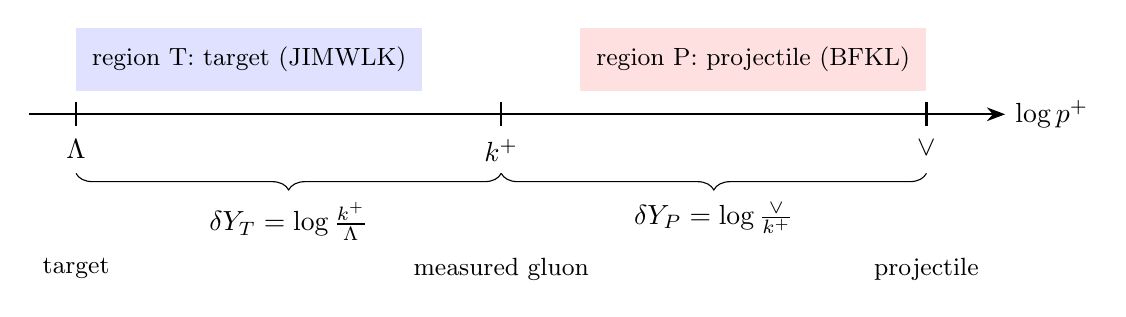
\begin{tikzpicture}[>=Stealth,scale=1.0]
\draw[->,thick] (0,0) -- (12.4,0) node[right] {$\log p^+$};
\foreach \x/\lab in {0.6/\Lambda, 6.0/k^+, 11.4/\vee}{
  \draw[thick] (\x,0.15) -- (\x,-0.15);
  \node[below] at (\x,-0.2) {$\lab$};}
\fill[blue!12] (0.6,0.3) rectangle (5.0,1.1);
\fill[red!12] (7.0,0.3) rectangle (11.4,1.1);
\node at (2.8,0.7) {\small region T: target (JIMWLK)};
\node at (9.2,0.7) {\small region P: projectile (BFKL)};
\draw[decorate,decoration={brace,amplitude=6pt,mirror}] (0.6,-0.75) -- (6.0,-0.75) node[midway,below=7pt] {$\delta Y_T=\log\frac{k^+}{\Lambda}$};
\draw[decorate,decoration={brace,amplitude=6pt,mirror}] (6.0,-0.75) -- (11.4,-0.75) node[midway,below=7pt] {$\delta Y_P=\log\frac{\vee}{k^+}$};
\node[below] at (0.6,-1.7) {\small target};
\node[below] at (11.4,-1.7) {\small projectile};
\node[below] at (6.0,-1.7) {\small measured gluon};
\end{tikzpicture}
\caption{The rapidity interval of the soft window. The unobserved gluon gives a large logarithm only when it is much softer (region T) or much harder (region P) than the measured gluon. At mid rapidity both $\delta Y_T$ and $\delta Y_P$ are large.}
\label{fig:rapidity}
\end{figure}

\paragraph*{The leading-log wave function.} Denote by
\begin{equation}
j^a_q(s)\equiv\sum_i a^{b\dagger}_i(q^+,s)\,(T^a)_{bc}\,a^c_i(q^+,s)
\label{eq:jdef}
\end{equation}
the colour charge density of the gluons with plus momentum $q^+$. It obeys the same algebra as $\rho$, $[j^a(x),j^b(y)]=if^{abc}j^c(x)\delta^{(2)}(x-y)$, and rotates in the same way, $S^\dagger j^a(x)S=U^{ab}(x)j^b(x)$ (using $U^TT^aU=U^{ab}T^b$). The emission of gluons with momentum $q^+$ by a colour source $J$ is generated by
\begin{equation}
\Omega_q[J]=\exp\Big\{i\varepsilon_q\sum_{e,j}\int_{z,s}\KK^j(s-z)\,J^e(s)\,\big(a^e_j(q^+,z)+a^{e\dagger}_j(q^+,z)\big)\Big\},\qquad \varepsilon_q^2\ \leftrightarrow\ \frac{\alpha_s}{\pi^2}\,\frac{dq^+}{q^+},
\label{eq:OmegaLL}
\end{equation}
with the modes normalized per bin of $\log q^+$. The normalization of $\varepsilon_q$ is that of Eq.~\eqref{eq:A1X}: to first order $\Omega_q[\rho]|0\rangle$ reproduces Eq.~\eqref{eq:LOwf}, and each emission costs $\frac{\alpha_s}{\pi^2}\frac{dq^+}{q^+}$, as noted after Eq.~\eqref{eq:LO}. At LL the full $\Omega$ factorizes into strongly ordered emissions, the harder gluon first:
\begin{equation}
\text{region T:}\quad \Omega=\Omega_p[\rho+j_k]\,\Omega_k[\rho],\qquad\qquad \text{region P:}\quad \Omega=\Omega_k[\rho+j_p]\,\Omega_p[\rho].
\label{eq:OmegaLLfact}
\end{equation}
The coefficients of Sec.~\ref{sec:omega} reproduce Eq.~\eqref{eq:OmegaLLfact} in the ordered limits. For example, Eq.~\eqref{eq:B2soft} is the order-$\varepsilon_k\varepsilon_p$ two-gluon term of $\Omega_p[\rho+j_k]\Omega_k[\rho]$. Its $\KK^j(w-z)$ term is the $j_k$ part of the source, and its $\frac12\KK^j(x-z)$ term is the commutator part of the product of the two $\rho$-emissions. Likewise $\mf C_1$ for $p^+\ll k^+$ (its $\delta_{jm}\delta_{ik}$ term) is the soft gluon emitted by the measured gluon after the target. The unitarity relation~\eqref{eq:unitB1} holds for Eq.~\eqref{eq:OmegaLLfact}.

\subsection{Region T: the JIMWLK Hamiltonian}\label{sec:T}

\paragraph*{Step 1: the cross section as an expectation value of the LO operator.} Insert $\Omega=\Omega_p[J]\,\Omega_k$, with $J\equiv\rho+j_k$, into Eq.~\eqref{eq:xsec}. With $N\equiv a^{a\dagger}_i(k^+,w)a^a_i(k^+,w')$ and $SS^\dagger=1$,
\begin{equation}
\langle0|\Omega^\dagger S^\dagger\Omega N\Omega^\dagger S\Omega|0\rangle=\langle\Psi|\,W^\dagger\,\bar M\,W\,|\Psi\rangle,\qquad W\equiv\bar\Omega_p^\dagger\Omega_p,\quad|\Psi\rangle\equiv\Omega_k|0\rangle,\quad\bar M\equiv S^\dagger\Omega_kN\Omega_k^\dagger S.
\label{eq:step1}
\end{equation}
Without the soft gluon, $W=1$, and $\langle\Psi|\bar M|\Psi\rangle$ is the LO cross section: it is the operator
\begin{equation}
\Ord(w,w')\equiv\int_{x,x'}\KK(x-w)\cdot\KK(x'-w')\,\rho^b(x)\Big[\big(\Ud(x)-\Ud(w)\big)\big(U(x')-U(w')\big)\Big]^{bb'}\rho^{b'}(x')
\label{eq:Oop}
\end{equation}
of Eq.~\eqref{eq:LOop}.

\paragraph*{Step 2: emission before and after the target.} Write $\Omega_p=e^{i\varepsilon G}$ with $G=\sum_{h,j}\int_zA^h_j(z)\,\alpha^h_j(z)$, where $\alpha\equiv a(p^+)+a^\dagger(p^+)$ and
\begin{equation}
A^h_j(z)\equiv\int_s\KK^j(s-z)\,J^h(s).
\end{equation}
Using $S^\dagger J^e(s)S=U^{eg}(s)J^g(s)$ and $S^\dagger\alpha^e(z)S=U^{eh}(z)\alpha^h(z)$, the rotated generator is $\bar G=\sum\int_zB^h_j(z)\,\alpha^h_j(z)$ with
\begin{equation}
B^h_j(z)\equiv\int_s\KK^j(s-z)\,\big[U^T(z)U(s)J(s)\big]^h=\int_s\KK^j(s-z)\,U^{eh}(z)U^{eg}(s)J^g(s).
\end{equation}
$A$ is the emission of the soft gluon before the target and $B$ its emission after the target. In both, the soft colour index $h$ refers to the frame before the target.

\paragraph*{Step 3: real and virtual terms.} To order $\varepsilon^2$,
\begin{equation}
W=e^{-i\varepsilon\bar G}e^{i\varepsilon G}=1+i\varepsilon(G-\bar G)-\frac{\varepsilon^2}{2}\big(G^2+\bar G^2\big)+\varepsilon^2\bar GG+\Ord(\varepsilon^3).
\end{equation}
$|\Psi\rangle$ contains no soft gluon, and $\langle0_p|\alpha^h_j(z)\alpha^{h'}_{j'}(z')|0_p\rangle=\delta^{hh'}\delta_{jj'}\delta^{(2)}(z-z')$. Write $X\cdot Y\equiv\sum_{h,j}\int_zX^h_j(z)Y^h_j(z)$ and
\begin{equation}
\gamma\equiv A-B .
\end{equation}
The order-$\varepsilon^2$ terms of Eq.~\eqref{eq:step1} are
\begin{align}
\text{REAL}={}&\varepsilon^2\,\langle\Psi|\,\gamma\cdot\bar M\,\gamma\,|\Psi\rangle,\label{eq:real}\\
\text{VIRTUAL}={}&\varepsilon^2\,\Big\langle\Psi\Big|\Big[-\tfrac12(A\cdot A+B\cdot B)+A\cdot B\Big]\bar M+\bar M\Big[-\tfrac12(A\cdot A+B\cdot B)+B\cdot A\Big]\Big|\Psi\Big\rangle.\label{eq:virt}
\end{align}
REAL has the soft gluon in the final state; it is the region-T part of Groups~II and~III. VIRTUAL has one gluon in the final state; it is the region-T part of Group~I. The sources $s$ in $A$ and $B$ run over the valence charges ($J=\rho$) and over the measured gluon ($J=j_k$).

\paragraph*{Step 4: real $+$ virtual is a double commutator.} Since
\begin{equation}
-\tfrac12[\gamma\cdot,[\gamma\cdot,\bar M]]=\gamma\cdot\bar M\gamma-\tfrac12\{A\cdot A+B\cdot B,\bar M\}+\tfrac12(A\cdot B+B\cdot A)\bar M+\tfrac12\bar M(A\cdot B+B\cdot A),
\end{equation}
we find
\begin{equation}
\text{REAL}+\text{VIRTUAL}=-\frac{\varepsilon^2}{2}\,\Big\langle\Psi\Big|\,[\gamma\cdot,[\gamma\cdot,\bar M]]+[[B\cdot,A\cdot],\bar M]\,\Big|\Psi\Big\rangle .
\label{eq:dc}
\end{equation}
The weights $(1,-2,1)$ of $\gamma\gamma\bar M$, $\gamma\bar M\gamma$ and $\bar M\gamma\gamma$ are those of the virtual terms, the real terms and the conjugate virtual terms.

\paragraph*{Step 5: colour charges act as derivatives on the Wilson lines.} Define the right and left rotation operators on functionals of $U$~\cite{JalilianMarian:1997gr,Kovner:2005nq},
\begin{equation}
J_R^a(u)\,U(x)=\delta^{(2)}(x-u)\,U(x)T^a,\qquad J_L^a(u)\equiv U^{ab}(u)J_R^b(u),\qquad J_L^a(u)\,U(x)=\delta^{(2)}(x-u)\,T^aU(x).
\label{eq:JRJL}
\end{equation}
\textbf{Lemma.} For every operator $X$ that does not depend on $U$,
\begin{equation}
J_R^a(u)\big(S^\dagger XS\big)=\big[S^\dagger XS,\,J^a(u)\big],\qquad J_L^a(u)\big(S^\dagger XS\big)=\big[S^\dagger XS,\,\bar J^a(u)\big],\qquad \bar J^a(u)\equiv U^{ab}(u)J^b(u).
\label{eq:dual}
\end{equation}
\emph{Proof.} $S^\dagger XS$ is built from the rotated fields $S^\dagger\rho^b(x)S=U^{bc}(x)\rho^c(x)$ and $S^\dagger a^b(x)S=U^{bc}(x)a^c(x)$. Both sides of Eq.~\eqref{eq:dual} obey the Leibniz rule, so it suffices to check them on these fields. For $\rho$, $J_R^a(u)\big(U^{bc}(x)\rho^c(x)\big)=\delta^{(2)}(x-u)\big(U(x)T^a\big)^{bc}\rho^c(x)$, while $\big[U^{bc}(x)\rho^c(x),\rho^a(u)\big]=U^{bc}(x)\,if^{cad}\rho^d(x)\,\delta^{(2)}(x-u)=\delta^{(2)}(x-u)U^{bc}(x)(T^a)_{cd}\rho^d(x)$. The two are equal. The gluon fields work in the same way with $j$. The $J_L$ form follows by multiplying with $U^{ab}(u)$. $\square$

Write $Y^g(s)\equiv J_R^g(s)\bar M=[\bar M,J^g(s)]$ and $Z^m(s)\equiv J_L^m(s)\bar M=[\bar M,\bar J^m(s)]$. Then $Z^m(s)=S^\dagger[X,J^m(s)]S$ has the form required by the lemma, while $Y^g(s)=U^{mg}(s)S^\dagger[X,J^m(s)]S$ contains an explicit $U(s)$, so that
\begin{equation}
[Y^g(s'),J^{g'}(s)]=J_R^{g'}(s)\,Y^g(s')-\delta^{(2)}(s-s')\,(T^{g'})_{kg}\,Y^k(s').
\label{eq:extra}
\end{equation}

\paragraph*{Step 6: the double commutators.} With $A^h=\int_s\KK(s-z)J^h(s)$, $B^h=\int_s\KK(s-z)U^{mh}(z)\bar J^m(s)$ and the shorthand $\iint\equiv\int_z\int_{s,s'}\KK(s-z)\cdot\KK(s'-z)$:
\begin{align}
[A,[A,\bar M]]&=\iint J_R^h(s)J_R^h(s')\,\bar M,\\
[B,[B,\bar M]]&=\iint J_L^m(s)J_L^m(s')\,\bar M,\\
[A,[B,\bar M]]&=\iint U^{mh}(z)\,J_R^h(s)J_L^m(s')\,\bar M,\\
[B,[A,\bar M]]&=\iint U^{mh}(z)\,J_L^m(s)J_R^h(s')\,\bar M+\int_z\int_s\KK(s-z)^2\,\Tr\big[\Ud(z)U(s)T^k\big]J_R^k(s)\,\bar M,\\
[[B,A],\bar M]&=\int_z\int_s\KK(s-z)^2\,\Tr\big[\Ud(z)U(s)T^k\big]J_R^k(s)\,\bar M.
\end{align}
In the first line the extra term of Eq.~\eqref{eq:extra} is proportional to $(T^h)_{kh}=0$. The trace term in the fourth line comes from Eq.~\eqref{eq:extra} with $U^{mh}(z)U^{mg}(s)(T^g)_{kh}=-\Tr[\Ud(z)U(s)T^k]$. In the last line we used $[B^h,A^h]=\int_s\KK(s-z)^2U^{mh}(z)U^{mg}(s)\,if^{ghk}J^k(s)$. In the combination $[\gamma,[\gamma,\bar M]]+[[B,A],\bar M]$ the two trace terms cancel, and
\begin{align}
\text{REAL}+\text{VIRTUAL}={}&-\frac{\varepsilon^2}{2}\int_z\int_{s,s'}K(s,s',z)\Big\{J_R^h(s)J_R^h(s')+J_L^m(s)J_L^m(s')\notag\\
&\hspace{9em}-U^{mh}(z)\big[J_R^h(s)J_L^m(s')+J_L^m(s)J_R^h(s')\big]\Big\}\langle\Psi|\bar M|\Psi\rangle .
\label{eq:HLR}
\end{align}
$|\Psi\rangle$ does not depend on $U$, so the derivatives act on the LO operator~\eqref{eq:Oop}. The points $s,s'$ run over the positions of its Wilson lines: the valence points $x,x'$ and the gluon points $w,w'$. A derivative at $w$ or $w'$ is the soft gluon emitted by the measured gluon.

\paragraph*{Step 7: identification with JIMWLK.} The JIMWLK Hamiltonian~\cite{JalilianMarian:1997jx,JalilianMarian:1997gr,JalilianMarian:1998cb,Kovner:2000pt,Weigert:2000gi,Iancu:2000hn,Ferreiro:2001qy} is
\begin{equation}
H_{\rm JIMWLK}=\frac{\alpha_s}{2\pi^2}\int_{t,u,v}K(u,v,t)\,\big[\Ud(u)-\Ud(t)\big]_{ce}J_R^c(u)\,\big[U(v)-U(t)\big]_{ed}J_R^d(v),
\label{eq:HJIMWLK}
\end{equation}
with every derivative acting on everything to its right. Using $[\Ud(u)]_{ce}J_R^c(u)=J_L^e(u)$, the integrand is $\big(J_L^e(u)-U^{ec}(t)J_R^c(u)\big)\big(J_L^e(v)-U^{ed}(t)J_R^d(v)\big)$, which expands to the bracket of Eq.~\eqref{eq:HLR}. With $\varepsilon^2=\frac{\alpha_s}{\pi^2}\delta Y_T$ we obtain
\begin{equation}
\boxed{\ \frac{d^3N}{d^3k}\bigg|_{\rm T}=-\,\delta Y_T\;H_{\rm JIMWLK}\,\frac{d^3N_{\rm LO}}{d^3k},\qquad \delta Y_T=\log\frac{k^+}{\Lambda}.\ }
\label{eq:Tresult}
\end{equation}
This is the target evolution $\partial_Y=-H_{\rm JIMWLK}$ of the LO spectrum over the interval below the measured gluon. When all $J_R$ in Eq.~\eqref{eq:HJIMWLK} are moved to the right of the Wilson lines, a term linear in $J_R$ appears; it is included automatically in Eq.~\eqref{eq:HLR}. The explicit action on Eq.~\eqref{eq:LO} is given in App.~\ref{app:explicit}.

\subsection{Region P: the BFKL equation}\label{sec:P}

Now $\Omega=\Omega_k[J']\,\Omega_p$ with $J'\equiv\rho+j_p$. The number operator $N$ involves only gluons with momentum $k^+$, so $[\Omega_p,N]=0$ and
\begin{equation}
\Omega N\Omega^\dagger=\Omega_k[J']\,N\,\Omega_k^\dagger[J'].
\end{equation}
The cross section is therefore the LO calculation with the source $\rho$ replaced by $\rho+j_p$, evaluated in the evolved projectile $|\Phi\rangle\equiv\Omega_p|0\rangle$:
\begin{equation}
\langle\Ord\rangle\ \longrightarrow\ \big\langle\Phi\big|\,\Ord[\rho+j_p]\,\big|\Phi\big\rangle,\qquad|\Phi\rangle=\Big(1+i\varepsilon G-\tfrac{\varepsilon^2}{2}G^2+\dots\Big)|0\rangle,\qquad G=\int_{u,z}\KK^j(u-z)\rho^e(u)\,\alpha^e_j(z).
\end{equation}
Write $\Ord[J']=\int_{x,y}\KK(x-w)\cdot\KK(y-w')\,J'^b(x)\,\mathbb M^{bb'}(x,y)\,J'^{b'}(y)$ with $\mathbb M(x,y)\equiv(\Ud(x)-\Ud(w))(U(y)-U(w'))$. There are three types of order-$\varepsilon^2$ terms.

\paragraph*{(i) The $\rho\rho$ part.} This is the evolution of the charge correlator itself, with real and virtual parts,
\begin{align}
&\varepsilon^2\big\langle G\rho\mathbb M\rho G-\tfrac12\{G^2,\rho\mathbb M\rho\}\big\rangle\notag\\
&\qquad=-\frac{\varepsilon^2}{2}\int_z\int_{u,u'}K(u,u',z)\,\big[\rho^h(u),\big[\rho^h(u'),\rho^b(x)\rho^{b'}(y)\big]\big]\,\mathbb M^{bb'}.
\end{align}
Using $(if^{hbc})(if^{hcd})=N_c\delta_{bd}$ and $(if^{hbc})(if^{hb'd})=(T^h)_{bc}(T^h)_{b'd}$,
\begin{align}
\text{(i)}={}&-\frac{\varepsilon^2}{2}\int_z\Big\{N_c\big[K(x,x,z)+K(y,y,z)\big]\rho^b(x)\rho^{b'}(y)\notag\\
&\hspace{5em}+2K(x,y,z)\,(T^h)_{bc}(T^h)_{b'd}\,\rho^c(x)\rho^d(y)\Big\}\mathbb M^{bb'}.
\end{align}
For a colour-diagonal correlator, $(T^h)_{bc}(T^h)_{b'c}=-N_c\delta_{bb'}$, and this becomes
\begin{equation}
-\frac{\varepsilon^2}{2}\,N_c\,K_D(x,y,z)\,\frac{\langle\rho^f(x)\rho^f(y)\rangle}{N_c^2-1}\,\Tr\,\mathbb M,
\end{equation}
with the dipole kernel
\begin{equation}
K_D(x,y,z)\equiv K(x,x,z)-2K(x,y,z)+K(y,y,z)=\frac{(x-y)^2}{(x-z)^2(y-z)^2}.
\label{eq:KD}
\end{equation}

\paragraph*{(ii) The $j_pj_p$ part: the measured gluon is emitted by the harder gluon.} With $j^{b'}(y)a^{e\dagger}(z)|0\rangle=\delta^{(2)}(y-z)(T^{b'})_{ge}a^{g\dagger}(z)|0\rangle$,
\begin{equation}
\text{(ii)}=\varepsilon^2\langle G\,j\,\mathbb M\,j\,G\rangle=\varepsilon^2\int_z\int_{u,u'}K(u',u,z)\,\rho^{e'}(u')\rho^e(u)\,(T^bT^{b'})_{e'e}\,\KK(z-w)\cdot\KK(z-w')\,\mathbb M^{bb'}(z,z).
\end{equation}
After the colour average, $\Tr(T^bT^{b'})=N_c\delta^{bb'}$.

\paragraph*{(iii) The $\rho\,j_p$ cross terms.}
\begin{equation}
\varepsilon^2\langle G\,\rho^b(x)\mathbb M^{bb'}j^{b'}(y)\,G\rangle=\varepsilon^2\int_z\int_{u,u'}K(u',u,z)\,\delta^{(2)}(y-z)\,\rho^{e'}(u')\rho^b(x)\rho^e(u)\,(T^{b'})_{e'e}\,\mathbb M^{bb'}(x,z).
\end{equation}
$K(u',u,z)$ is symmetric and $(T^{b'})_{e'e}$ is antisymmetric under $(e',u')\leftrightarrow(e,u)$, so the fully symmetric three-charge part \emph{vanishes exactly}. Only commutators survive:
\begin{equation}
\rho^{e'}(u')\rho^b(x)\rho^e(u)(T^{b'})_{e'e}\to\tfrac12N_c\,\delta^{(2)}(u-u')\,\rho^{b'}(u)\rho^b(x)+\delta^{(2)}(x-u)\,f^{beg}f^{b'e'e}\,\rho^{e'}(u')\rho^g(x).
\end{equation}
After the colour average this gives $\varepsilon^2N_c\KK(x-w)\cdot\KK(z-w')\big[\frac12K(y,y,z)-K(x,y,z)\big]$ times the trace with $\mathbb M(x,z)$, and the mirror term with $x\leftrightarrow y$, $w\leftrightarrow w'$.

\paragraph*{Result.} With $\varepsilon^2=\frac{\alpha_s}{\pi^2}\delta Y_P$, the sum (i)$+$(ii)$+$(iii) is the BFKL evolution of the projectile charge correlator in the LO spectrum:
\begin{equation}
\boxed{\ \frac{d^3N}{d^3k}\bigg|_{\rm P}=\delta Y_P\,\big[{\rm BFKL}\otimes{\rm LO}\big],\qquad \delta Y_P=\log\frac{\vee}{k^+},\ }
\label{eq:Presult}
\end{equation}
where ${\rm BFKL}\otimes{\rm LO}$ is Eq.~\eqref{eq:LOBFKL} of App.~\ref{app:explicit}. It is obtained by applying the coordinate-space BFKL equation for $\langle\rho^f(x)\rho^f(y)\rangle$, Eq.~\eqref{eq:vBFKL}, to the LO spectrum~\eqref{eq:LO}. Term (i) gives the line with $K_D$, (ii) the line with $\KK(z-w)\cdot\KK(z-w')$, and (iii) the two lines with $2K(x,y,z)-K(y,y,z)$ and $2K(x,y,z)-K(x,x,z)$. Term (i) contains Group~I (the $G^2$ normalization) and part of Groups~II and~III; (ii) and (iii) belong to Group~II.

\subsection{Cancellation of three- and four-charge terms}\label{sec:cancel}

\paragraph*{Region T.} The total is $-\delta Y_TH_{\rm JIMWLK}\Ord$. $H_{\rm JIMWLK}$ contains only $J_R$, $J_L$ and $U$, which act on Wilson lines and never change the number of charges. $\Ord$ has two charges, so the result has exactly two. Every three- and four-charge term of the real rows is cancelled by the corresponding virtual term. The mechanism is visible in Eq.~\eqref{eq:dc}.
\begin{itemize}
\item \emph{Four charges.} For the valence part of $\gamma$, treat the charges as commuting numbers. Then $\gamma\gamma\bar M-2\gamma\bar M\gamma+\bar M\gamma\gamma=0$.
\item \emph{Three charges.} Take the soft-gluon factor of a spectator charge, i.e.\ a charge not contained in $\bar M$. It commutes with $\bar M$ and with the other $\gamma$, so its double commutator vanishes. The real term $\varepsilon^2\gamma_{\rm spec}\{\bar M,\gamma_{\rm other}\}$ is cancelled exactly by the virtual term $-\varepsilon^2\gamma_{\rm spec}\{\bar M,\gamma_{\rm other}\}$. Only commutators with the charges of $\bar M$ survive, and they leave two charges.
\end{itemize}
\paragraph*{Region P.} Term (i) is a double commutator of two charges, which gives two charges, and (ii) has two. In (iii) the symmetric three-charge part vanishes by the antisymmetry shown above.

\subsection{Row-by-row leading logarithms}\label{sec:LLrows}

The derivation above uses only the factorized wave function~\eqref{eq:OmegaLLfact}. It can be compared row by row with Sec.~\ref{sec:xsec}. In each region, every coefficient reduces to a product of Weizs\"acker--Williams factors, as in Eqs.~\eqref{eq:B2soft} and~\eqref{eq:B2hard}. Inserting these limits into Eqs.~\eqref{eq:CS1}--\eqref{eq:CS3} gives the LL content of every row. The two-gluon amplitudes $\mathfrak B$, $\mathfrak X_{1,2}$, $\mathfrak C$ and the one-gluon corrections $\mathcal V_X$ at LL are listed in App.~\ref{app:LLrows}. Two points deserve mention.
\begin{itemize}
\item In Group~I the unitarity rewriting of $\bar{\mf A}^{(3)\dagger}_1$ distributes one physical term over Rows G1-II to G1-V. At LL their sum is a single simple term, listed as G1-II(b) in App.~\ref{app:LLrows}. It contains the commutator $[\bar{\mf N}_2,\bar{\mf A}^{(1)}]$ of Eq.~\eqref{eq:VII}.
\item Row G1-I$'$, the soft gluon emitted and reabsorbed after the target by a measured gluon that was produced before the target, is needed. Without it the parts of $H_{\rm JIMWLK}\Ord$ with the kernels $K(w,w,z)$, $K(w',w',z)$, $K(x',w,z)$ and $K(x,w',z)$ are not reproduced.
\end{itemize}
We fully symmetrized all products of charges (Weyl ordering plus commutator terms) and compared the rows term by term. In region T, all 12 classes of four-charge terms and all 63 classes of three-charge terms cancel among the rows. Of the two-charge classes, 137 cancel and 40 survive. In region P, 12 four-charge and 43 three-charge classes cancel; of the two-charge classes 105 cancel and 32 survive. Grouped by kernel, the survivors are exactly Eq.~\eqref{eq:HLR} in region T (8 kernels) and the terms (i)--(iii) in region P (8 kernels). The checks are described in App.~\ref{app:checks}.

\subsection{Result at mid rapidity}\label{sec:LLresult}

Adding the two regions,
\begin{equation}
\boxed{\ \frac{d^3N}{d^3k}\bigg|_{\rm LL}=\log\frac{\vee}{k^+}\,\big[{\rm BFKL}\otimes{\rm LO}\big]+\log\frac{k^+}{\Lambda}\,\big[{\rm JIMWLK}\otimes{\rm LO}\big],\ }
\label{eq:LLmain}
\end{equation}
with ${\rm JIMWLK}\otimes{\rm LO}\equiv-H_{\rm JIMWLK}\,\frac{d^3N_{\rm LO}}{d^3k}$ and BFKL$\otimes$LO given by Eq.~\eqref{eq:LOBFKL}.
This is the expected rapidity factorization of single inclusive production~\cite{Kovchegov:2001sc,Baier:2005dv,Kovner:2006ge,Kovner:2006wr,Gelis:2008rw}, here obtained directly from the $\Ord(g^4)$ cross section. At mid rapidity both logarithms are large and both evolutions must be resummed: the projectile charge correlator over $\log(\vee/k^+)$ and the target over $\log(k^+/\Lambda)$.

Using the first identity of Eq.~\eqref{eq:logid}, Eq.~\eqref{eq:LLmain} can be rewritten as
\begin{equation}
\frac{d^3N}{d^3k}\bigg|_{\rm LL}=\log\frac{\vee}{\Lambda}\,\big[{\rm JIMWLK}\otimes{\rm LO}\big]+\log\frac{\vee}{k^+}\,\Big(\big[{\rm BFKL}\otimes{\rm LO}\big]-\big[{\rm JIMWLK}\otimes{\rm LO}\big]\Big).
\end{equation}
So the coefficient of the total interval $\log(\vee/\Lambda)$ is JIMWLK$\otimes$LO alone. BFKL$\otimes$LO is the coefficient of $\log\vee$ at fixed $\Lambda$ and $k^+$. It would be incorrect to compare the coefficient of $\log(\vee/\Lambda)$ with the sum BFKL$\otimes$LO$+$JIMWLK$\otimes$LO.
%% <<< end sec6_LL.tex
%% >>> begin sec7_finite.tex
%% ===================================================================
\section{The finite part}\label{sec:finite}
%% ===================================================================

\subsection{Definition}\label{sec:findef}

Every row of Sec.~\ref{sec:xsec} has the form $\int dp^+\,I_{\rm row}(p^+)$, with $p^+$ the plus momentum of the unobserved or virtual gluon. We define its finite part by the exact subtraction
\begin{equation}
\frac{d^3N^{\rm fin}_{\rm row}}{d^3k}\equiv\frac{d^3N_{\rm row}}{d^3k}-\delta Y_T\,\mathfrak T_{\rm row}-\delta Y_P\,\mathfrak P_{\rm row},\qquad \mathfrak T_{\rm row}=\lim_{p^+\to0}p^+I_{\rm row},\quad \mathfrak P_{\rm row}=\lim_{p^+\to\infty}p^+I_{\rm row}.
\label{eq:findef}
\end{equation}
$\mathfrak T_{\rm row}$ and $\mathfrak P_{\rm row}$ depend neither on $\Lambda$ nor on $\vee$, and $d^3N^{\rm fin}_{\rm row}$ has a finite limit for $\Lambda\to0$, $\vee\to\infty$. Since $\vee$ is a physical, finite cutoff (the boundary between the soft window and the valence modes), we keep every function of $k^+/\vee$ exactly. We also keep the functions of $\Lambda/k^+$ that vanish as $\Lambda\to0$, so that every equation below is an exact identity. The three small logarithms that occur are
\begin{equation}
\lV\equiv\log\Big(1-\frac{k^+}{\vee}\Big),\qquad \lL\equiv\log\Big(1-\frac{\Lambda}{k^+}\Big),\qquad \lLb\equiv\log\Big(1+\frac{\Lambda}{k^+}\Big).
\label{eq:smalllogs}
\end{equation}
Summed over the rows, $\mathfrak T$ and $\mathfrak P$ give JIMWLK$\otimes$LO and BFKL$\otimes$LO of Sec.~\ref{sec:LL}. The finite part of the cross section is $\sum_{\rm rows}d^3N^{\rm fin}_{\rm row}$.

\paragraph*{Two practical rules.}
\begin{itemize}
\item[(A)] \emph{Rows in which the $p^+$ integral has been done.} Every longitudinal function $L$ is split as $L=c_T\,\delta Y_T+c_P\,\delta Y_P+L^{\rm fin}$, with $c_T,c_P$ numbers. The splits are collected in Table~\ref{tab:L} of App.~\ref{app:long}. Rapidity logarithms can be hidden in functions that look like logarithms of transverse distances. For example, with $a,b$ squared transverse distances, $\log\frac{(\vee-k^+)b+k^+a}{\Lambda b+k^+a}\to\log\frac{\vee}{k^+}+\log\frac{b}{a}$ for $\Lambda\ll k^+\ll\vee$, so it contains $\delta Y_P$.
\item[(B)] \emph{Rows left as plus-prescription integrals} (G1-V, G2-IV, G3-III, G3-V, G3-VI). The plus prescription removes the $p^+\to0$ end, and the accompanying endpoint logarithm gives $\mathfrak T$. The end $p^+\to\infty$ is still inside the integral, whose upper limit is $\vee-k^+$. Two mechanisms hide a $\delta Y_P$ there. The first is the plus prescription itself: with a phase under the integral,
\begin{equation}
\int_0^Pdp^+\,\frac{e^{-i\beta p^+}-1}{p^+}=-\log(|\beta|P)-\gamma_E-\frac{i\pi}{2}\,{\rm sgn}\,\beta+\Ord\Big(\frac{1}{\beta P}\Big).
\label{eq:phase}
\end{equation}
For $P=\vee-k^+$ and $\beta=\mathbf k\cdot(y'-z)/k^+$ this contains $-\delta Y_P-\lV-\log|\mathbf k\cdot(y'-z)|$. The second mechanism is a term that looks regular at large $p^+$ in the shifted variable $y'=z+\frac{k^+}{k^++p^+}(w'-z)$ but behaves as $1/p^+$ in the original variable $w'$. For these rows we give $\mathfrak P$ explicitly, and the finite part is Eq.~\eqref{eq:findef}.
\end{itemize}

\paragraph*{Principal value.} Several $p^+$ integrands have a simple pole inside the integration range, for example $1/[p^+(x-z)^2-k^+(x-w)^2]$ at $p^+=k^+(x-w)^2/(x-z)^2$. This pole is the energy denominator of the one-gluon state, and we define the integrals by their principal value. All logarithms of the results below are then to be read as $\log|\cdot|$. With a different prescription, terms $\pm i\pi$ times the coefficient of the pole would appear.

\paragraph*{Notation.} The measured gluon sits at $w$ in the amplitude and at $w'$ in its conjugate; the unobserved gluon sits at $z$. We use the shorthands
\begin{equation}
a\equiv(x-w)^2,\quad b\equiv(x-z)^2,\quad a'\equiv(x'-w')^2,\quad b'\equiv(x'-z)^2,\quad Z^2\equiv(z-w)^2,\quad Z'^2\equiv(z-w')^2,
\end{equation}
and $X\equiv x'-w'$, $Y\equiv y-z$ where indicated. Each row is written as the term displayed, plus its complex conjugate where stated. The colour operators are given with the shorthand $U^{bc}\equiv U^{cb}$ of Sec.~\ref{sec:xsec}.

%% -------------------------------------------------------------------
\subsection{Group I}\label{sec:finiteG1}

\paragraph*{G1-I.} This row contains only four-charge terms, each proportional to exactly $\log(\vee/\Lambda)$. It has no finite part, apart from the edge term discussed in Sec.~\ref{sec:edge}.

\paragraph*{G1-II, part 1 (one-charge part of $\mf A^{(3)}$).} The rapidity logarithms of Eq.~\eqref{eq:grho} combine according to Eq.~\eqref{eq:grhologs} into $-2\delta Y_T+\lV$; there is no $\delta Y_P$. The finite part is
\begin{align}
\frac{d^3N^{\rm fin}_{\rm II,1}}{d^3k}={}&\frac{1}{(2\pi)^3}\frac{g^4N_c}{32\pi^4k^+}\int_{w,w',x,x'}e^{-ik\cdot(w'-w)}\,K_{\rm LO}\,\Bigg\{\Big[-\frac2\epsilon-2\gamma_E-\log\frac{(x-w)^2\bar\mu^2}{4}\Big]\Big[\frac{11}{3}+\lV\Big]\notag\\
&\hspace{10em}-\frac{67}{9}+\frac{\pi^2}{3}+\lV^2+\lV\log\frac{\vee}{k^+}\Bigg\}\,\Ord_{\rm LO}+{\rm c.c.},
\label{eq:finII1}
\end{align}
and the subtracted part is the same expression with the curly bracket replaced by $-2\delta Y_T\big[-\frac2\epsilon-2\gamma_E-\log\frac{(x-w)^2\bar\mu^2}{4}\big]$. The term $\lV\log(\vee/k^+)$ is a large logarithm times $\Ord(k^+/\vee)$; it is bounded and belongs to the finite part. Relative to the LO spectrum~\eqref{eq:LOrelab}, Eq.~\eqref{eq:finII1} is $-\frac{\alpha_sN_c}{4\pi}\{\dots\}$ per ordering. The $\frac{11}{3}$ term is the $\beta_0$ term and $-\frac{67}{9}+\frac{\pi^2}{3}$ the CMW constant (Sec.~\ref{sec:rc}).

\paragraph*{G1-II, part 2 (two-charge part of $\mf A^{(3)}$).} In the mixed representation of Eq.~\eqref{eq:grhorho}, with the Fourier variable called $\mathbf q$ to avoid confusion with the measured $\mathbf k$,
\begin{align}
\frac{d^3N^{\rm fin}_{\rm II,2}}{d^3k}={}&-\frac{1}{(2\pi)^3}\frac{g^4f^{abc}}{64\pi^6k^+}\int_{w,w'}e^{-ik\cdot(w'-w)}\int d^2\mathbf p\,d^2\mathbf q\notag\\
&\times\int_{x,y,x'}e^{i\mathbf q\cdot(w-y)}e^{i\mathbf p\cdot(y-x)}\frac{(x'-w')^i}{(x'-w')^2\,\mathbf p^2\mathbf q^2}\notag\\
&\times\Bigg[-2\mathbf q^i\log\frac{\mathbf p^2}{\mathbf q^2+(k^+/\vee)\,\mathbf p^2}-\frac{\mathbf p^2\mathbf q^i+\mathbf q^2\mathbf p^i}{(\mathbf q-\mathbf p)^2}\,\lV\notag\\
&\qquad+\frac{(2\mathbf p^2-2\mathbf q\cdot\mathbf p+\mathbf q^2)\mathbf q^i+\mathbf q^2\mathbf p^i}{(\mathbf q-\mathbf p)^2}\log\frac{(1-k^+/\vee)\,\mathbf q^2+(k^+/\vee)(\mathbf q-\mathbf p)^2}{(\mathbf q-\mathbf p)^2}\Bigg]\notag\\
&\times\Big[U^{ab'}(x')\rho^{b'}(x')-U^{ab'}(w')\rho^{b'}(x')\Big]\notag\\
&\times\Big[U^{ab}(w)\{\rho^b(x),\rho^c(y)\}-U^{bd}(x)U^{ce}(y)\{\rho^d(x),\rho^e(y)\}\Big]+{\rm c.c.}
\label{eq:finII2}
\end{align}
The subtracted part is $\delta Y_T$ times $-\frac{2\mathbf q^2\mathbf p^i+(\mathbf p^2-\mathbf q\cdot\mathbf p)\mathbf q^i}{(\mathbf q-\mathbf p)^2}-2\mathbf q^i$ in the square bracket. The coefficient of $\delta Y_P$ vanishes identically. Taking the six terms of the bracket of Eq.~\eqref{eq:grhorho} in order, they contribute $0$, $+2\mathbf q^i$, $-2\mathbf q^i$, $+\mathbf q^i$ (the fourth and fifth terms together) and $-\mathbf q^i$, which add up to zero. For $\vee\to\infty$ the square bracket becomes $-2\mathbf q^i\log\frac{\mathbf p^2}{\mathbf q^2}+\frac{(2\mathbf p^2-2\mathbf q\cdot\mathbf p+\mathbf q^2)\mathbf q^i+\mathbf q^2\mathbf p^i}{(\mathbf q-\mathbf p)^2}\log\frac{\mathbf q^2}{(\mathbf q-\mathbf p)^2}$.

\paragraph*{G1-III (rescattering, $\bar{\mf B}_3^\dagger\mf A$).} The colour operator, with the prefactor $f^{abd}$, is
\begin{equation}
\Ord_{\rm III}\equiv\Big[U^{ab'}(x')\rho^{b'}(x')-U^{ab'}(w')\rho^{b'}(x')\Big]\Big[U^{de}(x)U^{bc}(z)\rho^e(x)\rho^c(y)-U^{de}(x)U^{bc}(y)\rho^e(x)\rho^c(y)\Big].
\end{equation}
The row contains the three parts of $\mf B_3$ with one valence charge: the instantaneous term, the non-instantaneous terms of both orderings, and the commutator term. With $X=x'-w'$, $Y=y-z$ define the kernels
\begin{align}
&K_a=\frac{X\cdot Y\,(a+b)}{X^2Y^2(b-a)^2},\qquad K_b=\frac{X\cdot(x-w)\,(x-z)\cdot Y}{X^2Y^2\,ab},\notag\\
&K_c=\frac{X\cdot(x-w)\,Y\cdot(z-w)}{X^2Y^2Z^2\,a},\notag\\
&K_d=\frac{X\cdot Y\,(z-w)\cdot(x-z)\,a}{X^2Y^2Z^2(a-b)^2},\notag\\
&K_e=\frac{X\cdot Y\,(z-w)\cdot(x-w)\,b}{X^2Y^2Z^2(a-b)^2},\qquad K_f=\frac{X\cdot Y}{X^2Y^2Z^2},\notag\\
&K_{g1}=\frac{X\cdot(z-w)\,Y\cdot(x-w)}{X^2Y^2Z^2(a-b)},\qquad K_{g2}=\frac{X\cdot(x-w)\,Y\cdot(z-w)\,b}{X^2Y^2Z^2(a-b)a},\notag\\
&K_{g4}=\frac{X\cdot(z-w)\,Y\cdot(x-z)\,a}{X^2Y^2Z^2(a-b)b},\qquad K_{g5}=\frac{X\cdot(x-z)\,Y\cdot(z-w)}{X^2Y^2Z^2(a-b)},\notag\\
&\Sigma=K_{g1}-K_{g2}-K_{g4}+K_{g5}+K_e-K_d,\notag\\
&\KK_{\mathcal A}=\frac{1}{X^2Y^2Z^2}\Big[X\cdot(z-w)\,Y\cdot(x-w)+Y\cdot(z-w)\,X\cdot(x-z)\notag\\
&\hspace{6em}-\frac{c}{b}\,X\cdot(z-w)\,Y\cdot(x-z)-\frac{c}{a}\,Y\cdot(z-w)\,X\cdot(x-w)\Big],\notag\\
&\KK_4=\frac{1}{X^2Y^2Z^2}\Big[-\frac{X\cdot(z-w)\,Y\cdot(x-z)}{b}+\frac{Y\cdot(z-w)\,X\cdot(x-w)}{a}-X\cdot Y\Big],
\end{align}
with $c\equiv(x-w)\cdot(x-z)$. The longitudinal functions $\Lo^{\rm fin}$, $\Lop^{\rm fin}$, $\Lt$, $\Lf$ and the arctangent function $\mathcal A$ are defined in Table~\ref{tab:L}. The finite part of the sum of the three parts of $\mf B_3$ is
\begin{align}
\frac{d^3N^{\rm fin}_{\rm III}}{d^3k}={}&\pre\int_{x,y,z,x'}f^{abd}\,\frac{ig^4}{16\pi^5k^+}\Big[K_a\big(\Lo^{\rm fin}+\Lt-\lV+\lL\big)\notag\\
&\hspace{6em}-2K_b\,\Lop^{\rm fin}-2\lLb\,K_c\notag\\
&\hspace{6em}+2(\lL-\lV)(K_d-K_e)-2\lL\,K_f\notag\\
&\hspace{6em}-2\big(\Lo^{\rm fin}+\Lt\big)\Sigma+2\,\mathcal A\,\KK_{\mathcal A}+\Lf\,\KK_4\Big]\Ord_{\rm III}+{\rm c.c.},
\label{eq:finIII}
\end{align}
and the subtracted part is
\begin{align}
&\pre\int_{x,y,z,x'}f^{abd}\,\frac{ig^4}{16\pi^5k^+}\notag\\
&\qquad\times\Big\{\delta Y_T\big[K_b-2K_f\big]+\delta Y_P\big[-K_b+2K_c-2(K_{g1}-K_{g2}-K_{g4}+K_{g5})\big]\Big\}\Ord_{\rm III}+{\rm c.c.}
\label{eq:LLIII}
\end{align}
Three remarks.
\begin{itemize}
\item \emph{No power-like terms.} Each part of $\mf B_3$ separately produces terms proportional to $1/\Lambda$, $1/(k^+-\Lambda)$ and $1/(\vee-k^+)$ with the kernel $K_1=X\cdot Y/[X^2Y^2(b-a)]$. They come from the double pole $(p^+-k^+)^{-2}$ at the two edges of the excluded window. In units of $\frac{ig^4f^{abd}}{16\pi^5}K_1\Ord_{\rm III}$ they are
\begin{equation}
\underbrace{2\Big[\frac1\Lambda-\frac{1}{\vee-k^+}\Big]+2\Big[\frac1\Lambda-\frac{1}{k^+-\Lambda}\Big]}_{\text{instantaneous}}\ \underbrace{-2\Big[\frac1\Lambda-\frac{1}{\vee-k^+}\Big]}_{\text{non-inst., }p^+>k^+}\ \underbrace{-2\Big[\frac1\Lambda-\frac{1}{k^+-\Lambda}\Big]}_{\text{non-inst., }p^+<k^+}=0 .
\label{eq:powercancel}
\end{equation}
The cancellation is a direct consequence of the endpoint condition~\eqref{eq:endpoint}. With the opposite sign of the $p^+>k^+$ non-instantaneous term, the sum would be $\frac{4}{\Lambda}+\dots$.
\item \emph{Rapidity logarithms.} The logarithm $\log\frac{\vee-k^+}{\Lambda}$ that multiplies $K_a$ is compensated by the logarithms hidden in $\Lo$ and $\log\frac{\Lambda}{k^+-\Lambda}$, so $K_a$ appears in neither $\mathfrak T$ nor $\mathfrak P$. The term $K_b\,\delta Y_T$ comes from $p^+\to\Lambda$ in the commutator part of $\mf B_3$ and is a genuine region-T logarithm. The term $-2K_f\,\delta Y_T$ instead comes from the edge $p^+\to k^+-\Lambda$ of the excluded window. It is not a rapidity logarithm and must cancel against the diagonal row G1-I$'$.
\note{To be verified once G1-I$'$ is computed beyond LL.}
\item \emph{Limits.} For $\Lambda\to0$, $\vee\to\infty$: $\Lo^{\rm fin}+\Lt\to\log\frac{b}{a}$, $\Lop^{\rm fin}\to\log\frac ba$, $\Lf\to\log\frac{Z^2}{a}$, and the small logarithms~\eqref{eq:smalllogs} vanish. The finite part~\eqref{eq:finIII} converges to a constant; numerically, at a test configuration, the sequence $(\Lambda,\vee)=(10^{-3},10^2),\dots,(10^{-9},10^8)$ gives $-0.78910$, $-0.78204$, $-0.78197$, $-0.78197$ (App.~\ref{app:checks}).
\end{itemize}

\paragraph*{G1-IV ($\bar{\mf A}^\dagger\mf B_2$).} The colour operator is
\begin{align}
\Ord_{\rm IV}\equiv{}&\Big[U^{ab'}(x')\rho^{b'}(x')-U^{ab'}(w')\rho^{b'}(x')\Big]\notag\\
&\times\Big[f^{cdc'}U^{ac}(w)U^{bd}(z)U^{be}(y)\rho^e(y)\rho^{c'}(x)-f^{abc}U^{be}(y)U^{cd}(x)\rho^e(y)\rho^d(x)\Big].
\end{align}
The $p^+$ integral of the $\mf B_2$ structure appears again in G2-I and in G3-I, II. Define
\begin{align}
J_1^{ij}(x,z,w)&=\frac{(x-z)^j(z-w)^i}{Z^2\,b}-\frac{(x-w)^i(z-w)^j}{Z^2\,a}-\frac{(x-z)^j(x-w)^i}{ab}+\frac{\delta^{ij}}{2Z^2},\notag\\
J_2^{ij}(x,z,w)&=\KK^i(x-w)\Big[\KK^j(z-w)+\tfrac12\KK^j(x-z)\Big],\notag\\
\mathfrak P_{\mf B}^{ij}(x,z,w)&=\KK^j(x-z)\Big[\KK^i(z-w)-\tfrac12\KK^i(x-w)\Big].
\label{eq:J12}
\end{align}
The $p^+$ integral over $(\Lambda,\vee-k^+)$ gives $\frac{1}{k^+}\mathfrak F^{ij}$, with
\begin{equation}
\mathfrak F^{ij}=\Lp(a,b)\,J_1^{ij}-\frac12\log\frac{\vee}{\Lambda+k^+}\,\frac{\delta^{ij}}{Z^2}+\log\frac{\vee-k^+}{\Lambda}\,J_2^{ij}=\delta Y_T\,J_2^{ij}+\delta Y_P\,\mathfrak P_{\mf B}^{ij}+\mathfrak F^{{\rm fin},ij},
\label{eq:Fcal}
\end{equation}
\begin{equation}
\boxed{\ \mathfrak F^{{\rm fin},ij}=\Lp^{\rm fin}(a,b)\,J_1^{ij}+\frac12\lLb\,\frac{\delta^{ij}}{Z^2}+\lV\,J_2^{ij}.\ }
\label{eq:Ffin}
\end{equation}
$J_2$ is the soft gluon $z$ emitted by the measured gluon or by its source [region T, Eq.~\eqref{eq:B2soft}], and $\mathfrak P_{\mf B}$ is the measured gluon emitted by the harder gluon at $z$ [region P, Eq.~\eqref{eq:B2hard}]. The finite part of G1-IV is
\begin{equation}
\frac{d^3N^{\rm fin}_{\rm IV}}{d^3k}=\pre\int_{x,y,z,x'}\frac{ig^4}{8\pi^5k^+}\,\frac{(x'-w')^i(y-z)^j}{(x'-w')^2(y-z)^2}\,\mathfrak F^{{\rm fin},ij}(x,z,w)\,\Ord_{\rm IV}+{\rm c.c.},
\label{eq:finIV}
\end{equation}
and the subtracted part is the same with $\mathfrak F^{\rm fin}\to\delta Y_TJ_2+\delta Y_P\mathfrak P_{\mf B}$.

\paragraph*{G1-V ($\bar{\mf C}^\dagger\mf B_2$, the loop across the target).} Here the parent gluon $k^+$ splits into $p^+$ and $k^+-p^+$, so $0<p^+<k^+$ and there is no region P. The row has two parts.

\emph{Part 1} has the colour operator
\begin{align}
\Ord_{\rm V}\equiv{}&\Big[U^{ab'}(x')\rho^{b'}(x')-U^{ab'}(w')\rho^{b'}(x')\Big]\notag\\
&\times\Big[f^{adc}U^{db}(x)U^{ce}(z)\{\rho^e(y),\rho^b(y')\}-f^{abc}U^{cd}(y)U^{be}(y')\{\rho^d(y),\rho^e(y')\}\Big].
\end{align}
After the $w$ integration with the $\delta$-function of $\mf C_1$, the plus prescription makes the $p^+$ integrals finite:
\begin{align}
\frac{d^3N^{\rm fin}_{\rm V,1}}{d^3k}={}&\frac{1}{(2\pi)^3}\int_{x,z,y,x',y',w'}\frac{ig^4}{16\pi^4}\Bigg\{\frac{1}{k^{+2}}\int_0^{k^+}\frac{dp^+}{2\pi}e^{-ik\cdot(w'-z)}e^{-ik\cdot(z-x)\frac{p^+}{k^+}}\notag\\
&\qquad\times\frac{(x'-w')^i(z-x)^m(y-z)^l(y'-x)^j}{(x'-w')^2(z-x)^2(y-z)^2(y'-x)^2}\notag\\
&\qquad\times\Big[\delta_{im}\delta_{jl}-\Big[\frac{k^+}{p^+}\Big]_+\delta_{jm}\delta_{il}\Big]\notag\\
&-\frac{1}{k^+}\int_0^{k^+}\frac{dq^+}{2\pi}e^{-ik\cdot(w'-x)}e^{-ik\cdot(x-z)\frac{q^+}{k^+}}\notag\\
&\qquad\times\frac{(x'-w')\cdot(y'-x)\,(z-x)\cdot(y-z)}{(x'-w')^2(z-x)^2(y-z)^2(y'-x)^2}\Big[\frac{1}{q^+}\Big]_+\Bigg\}\Ord_{\rm V}\notag\\
&-\frac{1}{(2\pi)^3}\frac{ig^4}{32\pi^5k^+}\,\lL\int_{x,z,y,x',y',w'}\notag\\
&\qquad\times\Bigg[e^{-ik\cdot(w'-z)}\frac{(x'-w')\cdot(y-z)\,(z-x)\cdot(y'-x)}{(x'-w')^2(z-x)^2(y-z)^2(y'-x)^2}\notag\\
&\hspace{12em}+e^{-ik\cdot(w'-x)}\frac{(x'-w')\cdot(y'-x)\,(z-x)\cdot(y-z)}{(x'-w')^2(z-x)^2(y-z)^2(y'-x)^2}\Bigg]\Ord_{\rm V}+{\rm c.c.}
\label{eq:finV1}
\end{align}
The subtracted part is the last two lines with $\lL\to\delta Y_T$.

\emph{Part 2} has two colour structures. They arise from $f^{adc}f^{fbe}U^{db}(x)U^{ce}(z)$ by adding and subtracting $N_cU^{af}(x)$:
\begin{equation}
\Ord_{\rm V2a}\equiv\big[U^{ab'}(x')-U^{ab'}(w')\big]\big[-f^{adc}f^{fbe}U^{db}(x)U^{ce}(z)+N_cU^{af}(x)\big]\rho^{b'}(x')\rho^f(y),
\end{equation}
\begin{equation}
\Ord_{\rm V2b}\equiv\big[U^{ab'}(x')-U^{ab'}(w')\big]\,N_c\big[U^{af}(y)-U^{af}(x)\big]\rho^{b'}(x')\rho^f(y).
\end{equation}
With $\xi=p^+/k^+$ and $\mathcal D\equiv p^+(y-x)^2+(k^+-p^+)(y-z)^2$, define the six transverse brackets
\begin{align}
\mathcal B_1^{im}&=\frac{\delta^{im}d_\perp}{2(x-z)^2}\big[(y-x)^2-(y-z)^2\big],\notag\\
\mathcal B_2^{im}&=\frac{(y-x)^i(x-z)^m}{(x-z)^2}-\frac{(y-x)^i(y-z)^m}{2(y-z)^2},\notag\\
\mathcal B_3^{im}&=\delta_{im}\Big[\frac{(y-z)\cdot(x-z)}{(x-z)^2}+\frac{(y-x)\cdot(y-z)}{2(y-x)^2}-\frac{(y-x)^2-(y-z)^2}{2(x-z)^2}\Big],\notag\\
\mathcal B_4^{im}&=\frac{(y-z)^i(x-z)^m}{(x-z)^2}+\frac{(y-x)^m(y-z)^i}{2(y-x)^2},\notag\\
\mathcal B_5^{im}&=\delta_{im}\Big[\frac{(y-x)\cdot(x-z)}{(x-z)^2}-\frac{(y-x)\cdot(y-z)}{2(y-z)^2}-\frac{(y-x)^2-(y-z)^2}{2(x-z)^2}\Big],\notag\\
\mathcal B_6^{im}&=\frac{(y-x)^m(x-z)^i}{(x-z)^2}-\frac{(y-x)^m(y-z)^i}{2(y-z)^2}+\frac{(y-z)^m(x-z)^i}{(x-z)^2}+\frac{(y-x)^i(y-z)^m}{2(y-x)^2}.
\label{eq:B16}
\end{align}
The integrand of part 2 is then $\xi(1-\xi)\mathcal B_1-\frac{\xi}{1-\xi}\mathcal B_2+(1-\xi)\mathcal B_3-\frac{1-\xi}{\xi}\mathcal B_4+\xi\mathcal B_5-\mathcal B_6$, contracted with $\frac{(x'-w')^i(z-x)^m}{(x'-w')^2(z-x)^2}$ and divided by $\mathcal D$. Its finite part for the structure $\Ord_{\rm V2a}$ is
\begin{align}
\frac{d^3N^{\rm fin}_{\rm V2a}}{d^3k}={}&\frac{1}{(2\pi)^3}\frac{g^4}{8\pi^4k^+}\int_{x,y,z,x',w'}\frac{(x'-w')^i(z-x)^m}{(x'-w')^2(z-x)^2}\notag\\
&\times\Bigg\{\int_0^{k^+}\frac{dp^+}{2\pi}\frac{e^{-ik\cdot(w'-z)}e^{-ik\cdot(z-x)\xi}}{\mathcal D}\Big[\xi(1-\xi)\mathcal B_1+(1-\xi)\mathcal B_3-\Big[\frac1\xi\Big]_+\mathcal B_4+\mathcal B_4+\xi\mathcal B_5-\mathcal B_6\Big]\notag\\
&\quad+\int_0^{k^+}\frac{dq^+}{2\pi}\frac{e^{-ik\cdot(w'-x)}e^{-ik\cdot(x-z)\frac{q^+}{k^+}}}{(k^+-q^+)(y-x)^2+q^+(y-z)^2}\Big\{-\Big[\frac{k^+}{q^+}\Big]_+\mathcal B_2+\mathcal B_2\Big\}\Bigg\}^{im}\Ord_{\rm V2a}\notag\\
&-\frac{1}{(2\pi)^3}\frac{g^4}{16\pi^5k^+}\,\lL\int_{x,y,z,x',w'}\Bigg[e^{-ik\cdot(w'-z)}\frac{(x'-w')^i(z-x)^m\mathcal B_4^{im}}{(x'-w')^2(z-x)^2(y-z)^2}\notag\\
&\hspace{12em}+e^{-ik\cdot(w'-x)}\frac{(x'-w')^i(z-x)^m\mathcal B_2^{im}}{(x'-w')^2(z-x)^2(y-x)^2}\Bigg]\Ord_{\rm V2a}+{\rm c.c.},
\label{eq:finV2a}
\end{align}
and the subtracted part is the last two lines with $\lL\to\delta Y_T$. The structure $\Ord_{\rm V2b}$ has exactly the same kernel, so the same formula with $\Ord_{\rm V2a}\to\Ord_{\rm V2b}$ gives its finite part.

Unlike $\Ord_{\rm V2a}$, the operator $\Ord_{\rm V2b}$ does not vanish at $x=z$, and part~2b is UV divergent at $x\to z$. In Sec.~\ref{sec:rc} we show that the coefficient of this divergence is the integral of the gluon splitting function. This is the $\beta_0$ term of the loop across the target. Part~2b therefore has to be regularized in the same scheme as G1-II ($d_\perp=2-\epsilon$) before its finite part can be written as a number times LO plus a finite remainder.
\note{G1-V part~2b in dimensional regularization, and its overall weight (the factor 2 in Eq.~\eqref{eq:VV} together with the c.c.), remain to be completed.}
%TODO: complete G1-V(2b) in dim. reg.; fix its overall weight.

\paragraph*{G1-I$'$.} As discussed in Sec.~\ref{sec:groupI}, the diagonal region of $\bar{\mf B}_3^\dagger$ is known here only at leading log. Its finite part is not included.

%% -------------------------------------------------------------------
\subsection{Group II}\label{sec:finiteG2}

\paragraph*{G2-I, part 1 (the $\{\rho,\rho\}$ part of $\mathfrak B$ times the $f$ part).} The colour operators are
\begin{align}
\Ord^{(1)}&\equiv\Big[U^{ac'}(w')\{\rho^{c'}(x'),\rho^b(y)\}-U^{bc'}(z)U^{ad'}(x')U^{c'e'}(y)\{\rho^{d'}(x'),\rho^{e'}(y)\}\Big]\notag\\
&\qquad\times\Big[f^{cbd}U^{ac}(w)\rho^d(x)-f^{acd}U^{bc}(z)U^{de}(x)\rho^e(x)\Big],\notag\\
\Ord^{(2)}&\equiv\Big[f^{c'bd'}U^{ac'}(w')\rho^{d'}(x)-f^{ac'd'}U^{bc'}(z)U^{d'e'}(x)\rho^{e'}(x)\Big]\notag\\
&\qquad\times\Big[U^{ac}(w)\{\rho^c(x'),\rho^b(y)\}-U^{bc}(z)U^{ad}(x')U^{ce}(y)\{\rho^d(x'),\rho^e(y)\}\Big].
\end{align}
Both have the $\mf B_2$ structure of Eq.~\eqref{eq:Fcal}:
\begin{align}
\frac{d^3N^{\rm fin}_{\rm II.I,1}}{d^3k}={}&\pre\int_{x,y,z,x'}\Bigg\{-\frac{ig^4}{16\pi^5k^+}\frac{(x'-w')^i(y-z)^j}{(x'-w')^2(y-z)^2}\,\mathfrak F^{{\rm fin},ij}(x,z,w)\,\Ord^{(1)}\notag\\
&\hspace{8em}+\frac{ig^4}{16\pi^5k^+}\frac{(x'-w)^i(y-z)^j}{(x'-w)^2(y-z)^2}\,\mathfrak F^{{\rm fin},ij}(x,z,w')\,\Ord^{(2)}\Bigg\}.
\end{align}

\paragraph*{G2-I, part 2 (the $f$ part of $\mathfrak B$, squared).} This is the initial-state splitting term. Before the $p^+$ integration it reads
\begin{align}
\frac{d^3N_{\rm II.I,2}}{d^3k}={}&\frac{1}{(2\pi)^3}\frac{g^4}{4\pi^4}\int_{\Lambda}^{\vee-k^+}\frac{dp^+}{2\pi}\int_{z,w,w',x,x'}e^{-ik\cdot(w'-w)}\notag\\
&\times\frac{p^+k^+}{(p^++k^+)^2}\,\frac{\Phi^{ij}(x,z,w)\,\Phi^{ij}(x',z,w')}{\big[p^+b+k^+a\big]\big[p^+b'+k^+a'\big]}\,\Ord_{\rm II.I},
\label{eq:GIIIpart2}\\
\Phi^{ij}(x,z,w)\equiv{}&\frac{\delta^{ij}(b-a)}{2Z^2}+\frac{p^++k^+}{k^+}\Big[\frac{(x-z)^j(z-w)^i}{Z^2}-\frac{(x-z)^j(x-w)^i}{2a}\Big]\notag\\
&+\frac{p^++k^+}{p^+}\Big[\frac{(x-w)^i(z-w)^j}{Z^2}+\frac{(x-z)^j(x-w)^i}{2b}\Big],\notag
\end{align}
with the colour operator
\begin{align}
\Ord_{\rm II.I}\equiv{}&f^{c'bd'}f^{cbd}U^{ac'}(w')U^{ac}(w)\rho^{d'}(x')\rho^d(x)-f^{c'bd'}f^{acd}U^{ac'}(w')U^{bc}(z)U^{de}(x)\rho^{d'}(x')\rho^e(x)\notag\\
&-f^{ac'd'}f^{cbd}U^{ac}(w)U^{bc'}(z)U^{e'd'}(x')\rho^{e'}(x')\rho^d(x)+N_cU^{e'd}(x')U^{de}(x)\rho^{e'}(x')\rho^e(x).
\end{align}
$\Phi^{ij}$ is the transverse bracket of $\mf B_2$, Eq.~\eqref{eq:B2X}. Expanding the product $\Phi\Phi$ in powers of $(p^++k^+)$ gives five transverse kernels: $\KK_A$ multiplies $\frac{(p^++k^+)^2}{p^+k^+}$, $\KK_B$ multiplies $\frac{(p^++k^+)^2}{p^{+2}}$, $\KK_C$ multiplies $\frac{(p^++k^+)^2}{k^{+2}}$, $\KK_D$ multiplies $\frac{p^++k^+}{p^+}$, $\KK_E$ multiplies $\frac{p^++k^+}{k^+}$. There is also a term $\frac{d_\perp}{4Z^2Z'^2}(b-a)(b'-a')$:
\begin{align}
\KK_A={}&\frac{(x-w)\cdot(z-w')\,(x'-z)\cdot(z-w)}{Z^2Z'^2}-\frac{(x-w)\cdot(x'-w')\,(z-w)\cdot(x'-z)}{2Z^2a'}\notag\\
&+\frac{(x-z)\cdot(x'-z)\,(x-w)\cdot(z-w')}{2bZ'^2}\notag\\
&-\frac{(x'-z)\cdot(x-z)\,(x'-w')\cdot(x-w)}{4ba'}+\frac{(x'-w')\cdot(z-w)\,(x-z)\cdot(z-w')}{Z^2Z'^2}\notag\\
&+\frac{(x'-w')\cdot(z-w)\,(x-z)\cdot(x'-z)}{2Z^2b'}\notag\\
&-\frac{(x-z)\cdot(z-w')\,(x'-w')\cdot(x-w)}{2aZ'^2}-\frac{(x'-w')\cdot(x-w)\,(x'-z)\cdot(x-z)}{4ab'},\notag\\
\KK_B={}&\frac{(x'-w')\cdot(x-w)\,(z-w)\cdot(z-w')}{Z^2Z'^2}+\frac{(x'-w')\cdot(x-w)\,(x'-z)\cdot(z-w)}{2Z^2b'}\notag\\
&+\frac{(x-w)\cdot(x'-w')\,(x-z)\cdot(z-w')}{2bZ'^2}\notag\\
&+\frac{(x-z)\cdot(x'-z)\,(x'-w')\cdot(x-w)}{4bb'},\notag\\
\KK_C={}&\frac{(x'-z)\cdot(x-z)\,(z-w)\cdot(z-w')}{Z^2Z'^2}-\frac{(x'-z)\cdot(x-z)\,(x'-w')\cdot(z-w)}{2Z^2a'}\notag\\
&-\frac{(x-w)\cdot(z-w')\,(x-z)\cdot(x'-z)}{2aZ'^2}\notag\\
&+\frac{(x-z)\cdot(x'-z)\,(x'-w')\cdot(x-w)}{4aa'},\notag\\
\KK_D={}&\frac{(x-w)\cdot(z-w)\,(b'-a')}{2Z^2Z'^2}+\frac{(x-z)\cdot(x-w)\,(b'-a')}{4bZ'^2}\notag\\
&+\frac{(x'-w')\cdot(z-w')\,(b-a)}{2Z^2Z'^2}+\frac{(x'-z)\cdot(x'-w')\,(b-a)}{4Z^2b'},\notag\\
\KK_E={}&\frac{(x-z)\cdot(z-w)\,(b'-a')}{2Z^2Z'^2}-\frac{(x-z)\cdot(x-w)\,(b'-a')}{4aZ'^2}\notag\\
&+\frac{(x'-z)\cdot(z-w')\,(b-a)}{2Z^2Z'^2}-\frac{(x'-z)\cdot(x'-w')\,(b-a)}{4Z^2a'}.
\label{eq:KAE}
\end{align}
The $p^+$ integral is elementary. With $D\equiv a'b-ab'$ and the functions of Table~\ref{tab:L}, the finite part is
\begin{align}
\frac{d^3N^{\rm fin}_{\rm II.I,2}}{d^3k}={}&\frac{1}{(2\pi)^3}\frac{g^4}{8\pi^5k^+}\int_{z,w,w',x,x'}e^{-ik\cdot(w'-w)}\Bigg\{\frac{\KK_A}{D}\Big[\Lp^{\rm fin}(a,b)-\Lp^{\rm fin}(a',b')\Big]\notag\\
&+\KK_B\Big[\frac{\lV}{aa'}-\frac{b}{aD}\Lp^{\rm fin}(a,b)+\frac{b'}{a'D}\Lp^{\rm fin}(a',b')\Big]+\KK_C\Big[\frac{a'}{b'D}\Lp^{\rm fin}(a',b')-\frac{a}{bD}\Lp^{\rm fin}(a,b)\Big]\notag\\
&+\KK_D\Big[\frac{\lLb}{(b-a)(a'-b')}+\frac{b}{(b-a)D}\Lp^{\rm fin}(a,b)+\frac{b'}{(a'-b')D}\Lp^{\rm fin}(a',b')\Big]\notag\\
&+\KK_E\Big[-\frac{\lLb}{(b-a)(a'-b')}-\frac{a}{(b-a)D}\Lp^{\rm fin}(a,b)-\frac{a'}{(a'-b')D}\Lp^{\rm fin}(a',b')\Big]\notag\\
&+\frac{d_\perp}{4Z^2Z'^2}\Big[-\lLb\frac{aa'-bb'}{(b-a)(b'-a')}-\frac{ab(b'-a')}{(b-a)D}\Lp^{\rm fin}(a,b)+\frac{a'b'(b-a)}{(b'-a')D}\Lp^{\rm fin}(a',b')\notag\\
&\hspace{8em}+k^+\Big(\frac1\vee-\frac{1}{k^++\Lambda}\Big)\Big]\Bigg\}\Ord_{\rm II.I},
\label{eq:finGIIpart2}
\end{align}
and the subtracted part is
\begin{equation}
\frac{1}{(2\pi)^3}\frac{g^4}{8\pi^5k^+}\int_{z,w,w',x,x'}e^{-ik\cdot(w'-w)}\Big[\delta Y_T\,\frac{\KK_B}{aa'}+\delta Y_P\,\frac{\KK_C}{bb'}\Big]\Ord_{\rm II.I}.
\end{equation}
The coefficients of $\delta Y_P$ in the $\KK_A$, $\KK_B$, $\KK_D$, $\KK_E$ and $d_\perp$ terms vanish identically; only $\KK_C$ keeps one, since $\frac{a'}{b'D}-\frac{a}{bD}=\frac{1}{bb'}$. The kernel $\KK_B/(aa')$ is the soft gluon $z$ emitted by the measured gluon or its source (region T), and $\KK_C/(bb')$ is the measured gluon emitted by the harder gluon at $z$ (region P). The last term, $k^+(\frac1\vee-\frac{1}{k^++\Lambda})=-(1-\frac{k^+}{\vee})+\Ord(\Lambda)$, is a genuine $\Ord(1)$ term. Alone it is singular at $z\to w$ and $z\to w'$, and it must be kept together with the other $d_\perp$ terms, whose $\Lp$ have the opposite singularity. For $|z-w|,|z-w'|\ll|x-z|,|x'-z|$ the integrand~\eqref{eq:GIIIpart2} is proportional to the gluon splitting function, see Sec.~\ref{sec:dglap}.

\paragraph*{G2-II, G2-III.} Only four-charge terms. No finite part apart from the edge term of Sec.~\ref{sec:edge}.

\paragraph*{G2-IV (fragmentation of the scattered gluon).} With the colour operator
\begin{equation}
\Ord_{\rm II.IV}\equiv\big[U^{e'c}(y')-U^{e'c}(x')\big]\big[U^{ec}(y)-U^{ce}(x)\big]\rho^{e'}(x')\rho^e(x),
\end{equation}
the $\delta$-functions of $\mf C_1$ put the parent gluon at $y$ ($y'$) and the measured gluon at $w=y+\frac{p^+}{k^+}(y-z)$. Integrating over $w,w'$ gives
\begin{align}
\frac{d^3N_{\rm II.IV}}{d^3k}={}&\frac{1}{(2\pi)^3}\frac{g^4N_c}{4\pi^4k^+}\int_{\Lambda}^{\vee-k^+}\frac{dp^+}{2\pi}\int_{z,x,x',y,y'}e^{-ik\cdot(y'-y)\frac{k^++p^+}{k^+}}\,\frac{(y-z)^m(x-y)^l(y'-z)^{m'}(x'-y')^{l'}}{(y-z)^2(x-y)^2(y'-z)^2(x'-y')^2}\notag\\
&\times\Big[\frac{\delta_{lm}\delta_{l'm'}d_\perp p^+}{(k^++p^+)^2}+\frac{2}{k^+}\big(\delta_{ml'}\delta_{m'l}-\delta_{m'l'}\delta_{lm}\big)+\frac{p^+}{k^{+2}}\delta_{mm'}\delta_{ll'}+\frac{1}{p^+}\delta_{mm'}\delta_{ll'}\Big]\Ord_{\rm II.IV}.
\label{eq:GIIIV}
\end{align}
In terms of the momentum fraction of the measured gluon in the splitting, $\xi\equiv k^+/(k^++p^+)$, which runs from $k^+/\vee$ to $k^+/(k^++\Lambda)$, the transverse integral over $z$ produces a collinear pole. Its coefficient is the real gluon splitting function
\begin{equation}
\mathcal P_{gg}(\xi)\equiv2N_c\Big[\frac{\xi}{(1-\xi)_+}+\frac{1-\xi}{\xi}+\xi(1-\xi)\Big],
\label{eq:Pgg}
\end{equation}
convoluted with the LO spectrum at the parent momentum $k/\xi$. With $K_{yy'}\equiv\frac{(x-y)\cdot(x'-y')}{(x-y)^2(x'-y')^2}$, $\bar\epsilon$ the $\MSbar$ pole of the $z$ integral and $\mu$ its scale, the result is
\begin{align}
\frac{d^3N_{\rm II.IV}}{d^3k}={}&\frac{1}{(2\pi)^3}\frac{g^4N_c}{8\pi^4k^+}\,\delta Y_T\int_{x,x',y,y'}e^{-ik\cdot(y'-y)}\notag\\
&\qquad\times K_{yy'}\Big[\frac{1}{\bar\epsilon}-\log\big(4\pi^2\mu^2(y'-y)^2\big)\Big]\Ord_{\rm II.IV}\notag\\
&+\frac{1}{(2\pi)^3}\frac{g^4}{8\pi^4k^+}\int_{k^+/\vee}^{1}\frac{d\xi}{\xi^2}\int_{x,x',y,y'}e^{-ik\cdot(y'-y)/\xi}\notag\\
&\qquad\times K_{yy'}\,\frac{\mathcal P_{gg}(\xi)}{2}\Big[\frac{1}{\bar\epsilon}+1-\log\big(4\pi^2\mu^2(y'-y)^2\big)\Big]\Ord_{\rm II.IV}\notag\\
&-\frac{1}{(2\pi)^3}\frac{g^4N_c}{8\pi^4k^+}\int_{k^+/\vee}^{1}\frac{d\xi}{\xi^2}\int_{x,x',y,y'}e^{-ik\cdot(y'-y)/\xi}\notag\\
&\qquad\times\Big[\frac{(x-y)\cdot(y'-y)\,(x'-y')\cdot(y'-y)}{(x-y)^2(x'-y')^2(y'-y)^2}\,d_\perp\,\xi(1-\xi)\notag\\
&\hspace{14em}+K_{yy'}\Big(\frac{\xi}{(1-\xi)_+}+\frac{1-\xi}{\xi}\Big)\Big]\Ord_{\rm II.IV}.
\label{eq:GIIIVres}
\end{align}
Since $\Ord_{\rm II.IV}=-\Ord_{\rm LO}\big|_{w\to y,\,w'\to y'}$, the structure $K_{yy'}\Ord_{\rm II.IV}$ is the integrand of the LO spectrum~\eqref{eq:LOrelab} with the gluon at the position $y$ ($y'$) of the parent. The $1/\bar\epsilon$ term of the second line is the order-$g^2$ part of a convolution of the LO spectrum with the bare gluon fragmentation function $D_{g/g}(\xi)=\delta(1-\xi)-\frac{\alpha_s}{2\pi}\frac{1}{\bar\epsilon}\mathcal P_{gg}(\xi)+\Ord(\alpha_s^2)$. Absorbing it into the renormalized fragmentation function is the final-state DGLAP step (Sec.~\ref{sec:dglap}).
\note{The overall sign and power of $\xi$ in the identification with $\int d\xi\,D_{g/g}(\xi)\,d^3N_{\rm LO}(k/\xi)$ depend on whether $d^3N/d^3k$ or the boost-invariant $k^+d^3N/d^3k$ is convoluted, and on the orientation of the $\xi$ integral; to be fixed in the final version.}
%TODO: fix the normalization (xi power, orientation) of the fragmentation-function identification in G2-IV.

The decomposition~\eqref{eq:findef} of G2-IV is as follows. The first line is the region-T term, $\delta Y_T\,\mathfrak T_{\rm II.IV}$. A region-P term is hidden at the lower end $\xi\to k^+/\vee$ of the $\xi$ integrals: the $\frac{1-\xi}{\xi}$ term of $\mathcal P_{gg}$ combines with the Fourier transform of $\log(y'-y)^2$ at momentum $k/\xi$, which is $\propto\xi^2/\mathbf k^2$, into $\int d\xi/\xi=\delta Y_P+\dots$. Directly from Eq.~\eqref{eq:GIIIV}, before the $z$ integration, one finds for $p^+\gg k^+$
\begin{align}
\mathfrak P_{\rm II.IV}={}&\frac{1}{(2\pi)^3}\frac{g^4N_c}{8\pi^5k^+}\int_{z,w,w',x,x'}e^{-ik\cdot(w'-w)}\big[\KK(w-z)\cdot\KK(w'-z)\big]\notag\\
&\times\big[\KK(x-z)\cdot\KK(x'-z)\big]\notag\\
&\times\big[U^{e'c}(z)-U^{e'c}(x')\big]\big[U^{ec}(z)-U^{ce}(x)\big]\rho^{e'}(x')\rho^e(x).
\label{eq:PIIIV}
\end{align}
This is the region-P term in which the harder gluon at $z$ emits the soft measured gluon. The finite part of G2-IV is Eq.~\eqref{eq:GIIIVres} minus its first line minus $\delta Y_P\,\mathfrak P_{\rm II.IV}$.

%% -------------------------------------------------------------------
\subsection{Group III}\label{sec:finiteG3}

\paragraph*{G3-I, G3-II.} Both have the $\mf B_2$ structure with the prefactor $-\frac{ig^4}{8\pi^5k^+}$:
\begin{equation}
\frac{d^3N^{\rm fin}_{\rm III.I(II)}}{d^3k}=-\pre\int_{x,y,z,x'}\frac{ig^4}{8\pi^5k^+}\frac{(x'-w')^i(y-z)^j}{(x'-w')^2(y-z)^2}\,\mathfrak F^{{\rm fin},ij}(x,z,w)\,\Ord_{\rm III.I(II)}+{\rm c.c.},
\end{equation}
with
\begin{align}
\Ord_{\rm III.I}&\equiv\Big[U^{ab'}(x')U^{c'd'}(y)U^{c'b}(z)\rho^{b'}(x')\rho^{d'}(y)-U^{bd'}(z)U^{d'e'}(y)U^{ac'}(w')\rho^{c'}(x')\rho^{e'}(y)\Big]\notag\\
&\qquad\times\Big[f^{cbd}U^{ac}(w)\rho^d(x)-f^{acd}U^{bc}(z)U^{de}(x)\rho^e(x)\Big],\notag\\
\Ord_{\rm III.II}&\equiv\Big[U^{c'd'}(y)U^{ab'}(x')U^{bc'}(z)\rho^{d'}(y)\rho^{b'}(x')-U^{ab'}(x')\rho^b(y)\rho^{b'}(x')\Big]\notag\\
&\qquad\times\Big[f^{cbd}U^{ac}(w)\rho^d(x)-f^{acd}U^{bc}(z)U^{de}(x)\rho^e(x)\Big].
\end{align}
The subtracted parts are $-\frac{ig^4}{8\pi^5k^+}\frac{(x'-w')^i(y-z)^j}{(x'-w')^2(y-z)^2}[\delta Y_TJ_2^{ij}+\delta Y_P\mathfrak P_{\mf B}^{ij}]\Ord_{\rm III.I(II)}$.

\paragraph*{G3-III ($\mathfrak C^\dagger\mathfrak B$), part 1.} With the colour operators
\begin{align}
\Ord_4&\equiv U^{e'c'}(y')U^{d'b}(z)\rho^{e'}(x')-U^{bd'}(z)U^{c'e'}(x')\rho^{e'}(x'),\notag\\
\Ord_5&\equiv U^{ac}(w)\{\rho^c(y),\rho^b(x)\}-U^{bc}(z)U^{ad}(y)U^{ce}(x)\{\rho^d(y),\rho^e(x)\},
\end{align}
and the prefactor $f^{c'd'a}$, the $w'$ integration with the $\delta$-function of $\mf C_1$ gives $w'=y'+\frac{p^+}{k^+}(y'-z)$, and the plus prescription gives
\begin{align}
\frac{d^3N_{\rm III.III,1}}{d^3k}={}&\mathcal I_1+\log\frac{\vee-k^+}{\Lambda}\,\mathfrak T_1,\notag\\
\mathcal I_1\equiv{}&-\frac{1}{(2\pi)^3}\frac{ig^4f^{c'd'a}}{8\pi^4k^+}\int_0^{\vee-k^+}\frac{dp^+}{2\pi}\int_{w,x',y',z,y,x}e^{-ik\cdot(y'-w)}e^{-ik\cdot(y'-z)\frac{p^+}{k^+}}\notag\\
&\times\frac{(y'-z)^m(x'-y')^{l'}(y-w)^i(x-z)^j}{(y'-z)^2(x'-y')^2(y-w)^2(x-z)^2}\notag\\
&\times\Big[\frac{\delta_{l'm}\delta_{ij}}{p^++k^+}-\Big[\frac{1}{p^+}\Big]_+\delta_{jm}\delta_{il'}-\frac{1}{k^+}\delta_{im}\delta_{jl'}\Big]\Ord_4\Ord_5,\notag\\
\mathfrak T_1\equiv{}&\frac{1}{(2\pi)^3}\frac{ig^4f^{c'd'a}}{16\pi^5k^+}\int_{w,x',y',z,y,x}e^{-ik\cdot(y'-w)}\notag\\
&\times\frac{(y'-z)\cdot(x-z)\,(x'-y')\cdot(y-w)}{(y'-z)^2(x'-y')^2(y-w)^2(x-z)^2}\,\Ord_4\Ord_5.
\label{eq:GIIIIII1}
\end{align}
The region-P coefficient comes from the $-\frac{1}{k^+}\delta_{im}\delta_{jl'}$ term written in the original variable $w'$ (rule B):
\begin{equation}
\mathfrak P_1=\frac{1}{(2\pi)^3}\frac{ig^4f^{c'd'a}}{16\pi^5k^+}\int_{w,w',x',z,y,x}e^{-ik\cdot(w'-w)}\frac{(w'-z)\cdot(y-w)\,(x'-z)\cdot(x-z)}{(w'-z)^2(x'-z)^2(y-w)^2(x-z)^2}\,\Ord_4\big|_{y'\to z}\,\Ord_5.
\end{equation}
The finite part is
\begin{equation}
\frac{d^3N^{\rm fin}_{\rm III.III,1}}{d^3k}=\mathcal I_1+\big(\delta Y_P+\lV\big)\mathfrak T_1-\delta Y_P\,\mathfrak P_1+{\rm c.c.},
\label{eq:finGIIIIII1}
\end{equation}
and the subtracted part is $\delta Y_T\mathfrak T_1+\delta Y_P\mathfrak P_1$. The two explicit $\delta Y_P$ terms cancel the two logarithms hidden inside $\mathcal I_1$: $-\delta Y_P\mathfrak T_1$ from the plus prescription with its phase, Eq.~\eqref{eq:phase}, and $+\delta Y_P\mathfrak P_1$ from the $\frac{1}{k^+}$ term. Equivalently, the finite part is $\mathcal I_1$ with its large-$p^+$ tail subtracted, plus $\lV\mathfrak T_1$.

\paragraph*{G3-III, part 2.} With $\Ord_6\equiv f^{c'd'a}\Ord_4$ and $\Ord_7\equiv f^{cbd}U^{ac}(w)\rho^d(x)-f^{acd}U^{bc}(z)U^{de}(x)\rho^e(x)$, the same steps give $\frac{d^3N_{\rm III.III,2}}{d^3k}=\mathcal I_2+\log\frac{\vee-k^+}{\Lambda}\mathfrak T_2$, where
\begin{align}
\mathcal I_2\equiv{}&-\frac{1}{(2\pi)^3}\frac{g^4}{4\pi^4}\int_0^{\vee-k^+}\frac{dp^+}{2\pi}\int_{w,y',z,y,x}e^{-ik\cdot(y'-w)}e^{-ik\cdot(y'-z)\frac{p^+}{k^+}}\notag\\
&\times\frac{(y'-z)^m(x'-y')^{l'}}{(y'-z)^2(x'-y')^2}\,\frac{1}{p^+b+k^+a}\notag\\
&\times\Bigg[\frac{\delta_{l'm}d_\perp p^+(b-a)}{2Z^2(p^++k^+)^2}\notag\\
&\quad+\frac{p^+\delta_{l'm}}{k^+(p^++k^+)}\Big[\frac{(x-z)\cdot(z-w)}{Z^2}-\frac{(x-z)\cdot(x-w)}{2a}-\frac{b-a}{2Z^2}\Big]\notag\\
&\quad+\frac{\delta_{l'm}}{p^++k^+}\Big[\frac{(x-w)\cdot(z-w)}{Z^2}+\frac{(x-z)\cdot(x-w)}{2b}-\frac{b-a}{2Z^2}\Big]\notag\\
&\quad-\Big[\frac{1}{p^+}\Big]_+\Big[\frac{(x-w)^{l'}(z-w)^m}{Z^2}+\frac{(x-z)^m(x-w)^{l'}}{2b}\Big]\notag\\
&\quad-\frac{p^+}{k^{+2}}\Big[\frac{(x-z)^{l'}(z-w)^m}{Z^2}-\frac{(x-z)^{l'}(x-w)^m}{2a}\Big]\notag\\
&\quad-\frac{1}{k^+}\Big[\frac{(x-z)^m(z-w)^{l'}}{Z^2}-\frac{(x-z)^m(x-w)^{l'}}{2a}\notag\\
&\hspace{4em}+\frac{(x-w)^m(z-w)^{l'}}{Z^2}+\frac{(x-z)^{l'}(x-w)^m}{2b}\Big]\Bigg]\Ord_6\Ord_7,\notag\\
\mathfrak T_2\equiv{}&\frac{1}{(2\pi)^3}\frac{g^4}{8\pi^5k^+}\int_{w,y',z,y,x}e^{-ik\cdot(y'-w)}\notag\\
&\times\Big[\frac{(x-w)\cdot(x'-y')\,(z-w)\cdot(y'-z)}{Z^2a\,(y'-z)^2(x'-y')^2}+\frac{(x-z)\cdot(y'-z)\,(x-w)\cdot(x'-y')}{2ba\,(y'-z)^2(x'-y')^2}\Big]\Ord_6\Ord_7.
\label{eq:GIIIIII2}
\end{align}
The region-P coefficient comes from the term $-\frac{p^+}{k^{+2}}[\dots]$, which in the variable $w'$ behaves as $-\frac{1}{k^+p^+b}[\dots]$:
\begin{align}
\mathfrak P_2={}&\frac{1}{(2\pi)^3}\frac{g^4}{8\pi^5k^+}\int_{w,w',z,x,x'}e^{-ik\cdot(w'-w)}\big[\KK(x'-z)\cdot\KK(x-z)\big]\notag\\
&\times\KK^m(w'-z)\Big[\KK^m(z-w)-\tfrac12\KK^m(x-w)\Big]\Ord_6\big|_{y'\to z}\Ord_7 .
\end{align}
All other terms of the bracket fall faster than $1/p^+$. The finite part is
\begin{equation}
\frac{d^3N^{\rm fin}_{\rm III.III,2}}{d^3k}=\mathcal I_2+\big(\delta Y_P+\lV\big)\mathfrak T_2-\delta Y_P\,\mathfrak P_2+{\rm c.c.}
\end{equation}
This part contains the \emph{interference} of the initial- and final-state collinear splittings (Sec.~\ref{sec:dglap}).

\paragraph*{G3-IV.} Only four-charge terms. No finite part apart from the edge term.

\paragraph*{G3-V, G3-VI.} Both have exactly the longitudinal structure of G3-III part 1, with twice its prefactor ($-\frac{ig^4f}{4\pi^4k^+}$ instead of $-\frac{ig^4f}{8\pi^4k^+}$). For G3-V the prefactor colour factor is $f^{c'ca}$ and the colour operators are
\begin{align}
\Ord'_3\equiv{}& U^{e'c'}(y')\rho^{e'}(x')-U^{c'e'}(x')\rho^{e'}(x'),\notag\\
\Ord'_4\equiv{}& U^{ce}(x)U^{ad}(y)\rho^e(x)\rho^d(y)-U^{ad}(w)U^{ce}(x)\rho^e(x)\rho^d(y).
\end{align}
For G3-VI the colour factor is $f^{c'd'a}$ and
\begin{align}
\Ord''_1\equiv{}&U^{e'c'}(y')U^{d'b}(z)\rho^{e'}(x')-U^{bd'}(z)U^{c'e'}(x')\rho^{e'}(x'),\notag\\
\Ord''_5\equiv{}& U^{bc}(z)U^{ad}(y)U^{ce}(x)\rho^d(y)\rho^e(x)-U^{ad}(y)\rho^d(y)\rho^b(x).
\end{align}
With $\mathcal I_{\rm V}$, $\mathcal I_{\rm VI}$ the plus-prescription integrals,
\begin{equation}
\frac{d^3N^{\rm fin}_{\rm III.V(VI)}}{d^3k}=\mathcal I_{\rm V(VI)}+\big(\delta Y_P+\lV\big)\mathfrak T_{\rm V(VI)}-\delta Y_P\,\mathfrak P_{\rm V(VI)}+{\rm c.c.},
\end{equation}
where $\mathfrak T_{\rm V(VI)}$ and $\mathfrak P_{\rm V(VI)}$ are $\mathfrak T_1$ and $\mathfrak P_1$ with the prefactor doubled and the colour operators replaced by those of the row.

%% -------------------------------------------------------------------
\subsection{Edge terms and three-charge terms}\label{sec:edge}

\paragraph*{Four charges.} All four-charge terms, and the three-charge terms obtained by reordering them, multiply $\log(\vee/\Lambda)$ in the virtual rows, where $\Lambda<p^+<\vee$. In the real rows, where $\Lambda<p^+<\vee-k^+$, they multiply $\log\frac{\vee-k^+}{\Lambda}=\log\frac{\vee}{\Lambda}+\lV$. Since the four-charge terms cancel between real and virtual rows at LL (Sec.~\ref{sec:cancel}), the finite part contains the edge term
\begin{equation}
\frac{d^3N^{\rm fin}_{4\rho}}{d^3k}=\lV\times\big[\text{four-charge terms of the real rows}\big]=-\lV\times\big[\text{four-charge terms of the virtual rows}\big].
\end{equation}
It is $\Ord(k^+/\vee)$ and vanishes for $\vee\to\infty$; since $\vee$ is finite, we keep it.

\paragraph*{Three charges.} The finite parts of G1-III, G1-IV, G1-V(1), G2-I(1), G3-I, G3-II, G3-III(1), G3-V and G3-VI are products of three charges. After complete symmetrization each splits into a symmetric three-charge part and two-charge commutator terms. At LL the symmetric parts cancel. For the finite part there is no such requirement: symmetric three-charge terms are legitimate NLO contributions. They vanish for a Gaussian (McLerran--Venugopalan) projectile, in which the odd moments of $\rho$ vanish, but not, for example, for a projectile of a few valence quarks ($d^{abc}$ structures).

%% -------------------------------------------------------------------
\subsection{Summary of the finite part}\label{sec:finsum}

Table~\ref{tab:fin} lists where the finite part of the cross section resides.

\begin{table}[!tbp]
\centering
\renewcommand{\arraystretch}{1.2}
\begin{tabular}{L{3.7cm}L{3.5cm}L{7.4cm}}
\toprule
Row & finite part & content\\
\midrule
G1-I, G2-II, G2-III, G3-IV & edge term only & $\lV\times$(four-charge terms)\\
G1-II(1) & Eq.~\eqref{eq:finII1} & $\beta_0$ (running coupling), CMW constant, $\lV$ terms\\
G1-II(2) & Eq.~\eqref{eq:finII2} & transverse logarithms; no $\delta Y_P$ at all\\
G1-III & Eq.~\eqref{eq:finIII} & transverse logarithms, arctangent; no $1/\Lambda$\\
G1-IV, G2-I(1), G3-I, G3-II & $\mathfrak F^{\rm fin}$, Eq.~\eqref{eq:Ffin} & $\Lp^{\rm fin}\to\log\frac{(x-z)^2}{(x-w)^2}$, $\lV$\\
G1-V(1), V(2a) & Eqs.~\eqref{eq:finV1}, \eqref{eq:finV2a} & plus-prescription integrals over $0<p^+<k^+$\\
G1-V(2b) & Sec.~\ref{sec:rc} & UV divergent: $\beta_0$ from the loop across the target\\
G2-I(2) & Eq.~\eqref{eq:finGIIpart2} & initial-state collinear splitting (projectile DGLAP)\\
G2-IV & Eq.~\eqref{eq:GIIIVres} & fragmentation: $D_{g/g}$, $\mathcal P_{gg}$, minus the hidden $\delta Y_P\mathfrak P_{\rm II.IV}$\\
G3-III(1), V, VI & Eq.~\eqref{eq:finGIIIIII1} & plus-prescription integrals with explicit $\delta Y_P$ counterterms\\
G3-III(2) & Eq.~\eqref{eq:GIIIIII2} & interference of initial- and final-state splitting\\
G1-I$'$ & not computed & diagonal $\bar{\mf B}_3^\dagger$\\
\bottomrule
\end{tabular}
\caption{Where the finite part of the NLO cross section resides.}
\label{tab:fin}
\end{table}
%% <<< end sec7_finite.tex
%% >>> begin sec8_rc_dglap.tex
%% ===================================================================
\section{Running coupling and DGLAP}\label{sec:rc}
%% ===================================================================

Throughout this section $d_\perp=2-\epsilon$, so that in the standard notation $D=4-2\epsilon_{\rm std}$ one has $\frac2\epsilon=\frac{1}{\epsilon_{\rm std}}$. We set $n_f=0$, so $\beta_0=\frac{11}{3}N_c$, and $\alpha_s=g^2/4\pi$.

\subsection{The splitting function}\label{sec:Phat}

The real part of the gluon splitting function~\cite{Gribov:1972ri,Altarelli:1977zs,Dokshitzer:1977sg} appears in every term that contains the splitting of one gluon into two. In the form in which it arises here,
\begin{equation}
\Phat(\xi)\equiv\xi(1-\xi)\frac{d_\perp}{2}+\frac{\xi}{1-\xi}+\frac{1-\xi}{\xi},\qquad \Phat(\xi)\Big|_{d_\perp=2}=\frac{P^{\rm real}_{gg}(\xi)}{2N_c},
\label{eq:Phat}
\end{equation}
where $P_{gg}(\xi)=2N_c\big[\frac{\xi}{(1-\xi)_+}+\frac{1-\xi}{\xi}+\xi(1-\xi)\big]+\frac{\beta_0}{2}\delta(1-\xi)$. The key identity is
\begin{equation}
\int_{\Lambda/k^+}^{1-\Lambda/k^+}d\xi\,\Phat(\xi)\Big|_{d_\perp=2}=2\log\frac{k^+}{\Lambda}-\frac{11}{6}+\Ord\Big(\frac{\Lambda}{k^+}\Big),\qquad\text{i.e.}\qquad \frac{\beta_0}{N_c}=\frac{11}{3}=-2\Big[\int d\xi\,\Phat-2\,\delta Y_T\Big].
\label{eq:intPhat}
\end{equation}
The same function therefore produces a rapidity logarithm (from its endpoints) and the $\beta_0$ coefficient (from its integral).

\subsection{\texorpdfstring{$\beta_0$}{beta0} from the gluon self-energy before the target (G1-II)}\label{sec:b0II}

In the self-energy of the emitted gluon, Eq.~\eqref{eq:grho}, the $\xi$-integrand of the gluon loop is $\big[-2+\xi(1-\xi)+\frac{1}{\xi(1-\xi)}\big]$. This is identically $\Phat(\xi)$ at $d_\perp=2$, because $\frac{1-\xi}{\xi}+\frac{\xi}{1-\xi}=\frac{1}{\xi(1-\xi)}-2$. By Eq.~\eqref{eq:intPhat} the coefficient $\frac{11}{3}+4\log\frac{\Lambda}{k^+}$ of the UV pole of the self-energy is exactly $-2\int d\xi\,\Phat$. The other one-loop diagrams of Eq.~\eqref{eq:grho}, in which the loop is attached to the valence charge, add $2\delta Y_T+\lV$ to this coefficient, which gives the total $\frac{11}{3}-2\delta Y_T+\lV$ of Eq.~\eqref{eq:grhologs}. Relative to LO, Eq.~\eqref{eq:finII1} together with its subtracted part is, per ordering,
\begin{equation}
\frac{\text{G1-II(1)}}{\rm LO}=-\frac{\alpha_sN_c}{4\pi}\Big\{\Big[-\frac2\epsilon-\log\frac{r^2\bar\mu^2e^{2\gamma_E}}{4}\Big]\Big(\frac{11}{3}-2\delta Y_T+\lV\Big)-\frac{67}{9}+\frac{\pi^2}{3}+\dots\Big\},\qquad r=|x-w|,
\end{equation}
and its $\beta_0$ part is
\begin{equation}
\frac{\alpha_s\beta_0}{4\pi}\Big[\frac{1}{\epsilon_{\rm std}}+\log\frac{r^2\bar\mu^2e^{2\gamma_E}}{4}\Big]\times{\rm LO}\qquad\text{per ordering (with $r'=|x'-w'|$ in the conjugate).}
\label{eq:b0II}
\end{equation}

\subsection{\texorpdfstring{$\beta_0$}{beta0} from the loop across the target (G1-V, part 2b)}\label{sec:b0V}

In G1-V the two gluons produced before the target recombine after it. The colour operator $\Ord_{\rm V2b}$ does not vanish when the two gluons coincide, and the row is UV divergent. To extract the coefficient, set $x=z+\mathbf r$ and let $\mathbf r\to0$. Then $\mathcal D\to k^+(y-z)^2$, the phase $e^{-ik\cdot(z-x)p^+/k^+}\to1$, and $\Ord_{\rm V2b}\to-N_c\Ord_{\rm LO}$ for a gluon at $z$ with source $y$. Averaged over the direction of $\mathbf r$, the six brackets of Eq.~\eqref{eq:B16} give, with $X=x'-w'$, $Y=y-z$, $\xi=p^+/k^+$,
\begin{align}
&\frac{X^i(z-x)^m}{(z-x)^2}\Big[\xi(1-\xi)\mathcal B_1-\tfrac{\xi}{1-\xi}\mathcal B_2+(1-\xi)\mathcal B_3-\tfrac{1-\xi}{\xi}\mathcal B_4+\xi\mathcal B_5-\mathcal B_6\Big]^{im}\notag\\
&\qquad\longrightarrow\frac{X\cdot Y}{r^2}\Big[\frac{d_\perp}{2}\xi(1-\xi)+\frac{\xi}{1-\xi}-(1-\xi)+\frac{1-\xi}{\xi}-\xi+1\Big]=\frac{X\cdot Y}{r^2}\,\Phat(\xi).
\end{align}
The six terms, in the order of the brackets, are $\frac{d_\perp}{2}\xi(1-\xi)$, $\frac{\xi}{1-\xi}$, $-(1-\xi)$, $\frac{1-\xi}{\xi}$, $-\xi$ and $+1$. With $\int dp^+=k^+\int d\xi$,
\begin{equation}
\frac{d^3N_{\rm V2b}}{d^3k}\bigg|_{\rm UV}=\frac{\alpha_sN_c}{2\pi}\Big[\int d\xi\,\Phat(\xi)\Big]\log\frac{R^2}{r_0^2}\times{\rm LO}=\frac{\alpha_sN_c}{2\pi}\Big[2\delta Y_T-\frac{11}{6}\Big]\log\frac{R^2}{r_0^2}\times{\rm LO},
\label{eq:2bUV}
\end{equation}
where LO refers to a gluon at $z$ with source $y$, $r_0$ is a short-distance cutoff ($\log\frac{1}{r_0^2}\leftrightarrow\frac{1}{\epsilon_{\rm std}}+\log\bar\mu^2$), and the upper cutoff $R$ of $|x-z|$ is set by the kernel ($|x-z|\lesssim|y-z|$) and by the phase ($|x-z|\lesssim1/(\xi|\mathbf k|)$).
\begin{itemize}
\item The $2\delta Y_T$ part is the UV-divergent form of a JIMWLK virtual term. It sits in the endpoint terms (the subtracted part of G1-V(2b)).
\item The $-\frac{11}{6}$ part is a $\beta_0$ term, $-\frac{\alpha_s\beta_0}{4\pi}\log\frac{R^2}{r_0^2}\times{\rm LO}$.
\end{itemize}
In the same cutoff language Eq.~\eqref{eq:b0II} reads $+\frac{\alpha_s\beta_0}{4\pi}\log\frac{r^2}{r_0^2}\times$LO. The loop before the target and the loop across the target therefore come with \emph{opposite} signs.

\subsection{Renormalization-group bookkeeping}\label{sec:RG}

With the bare coupling, ${\rm LO}(\alpha_0)={\rm LO}(\alpha_s(\mu))\big[1-\frac{\alpha_s\beta_0}{4\pi}\frac{1}{\epsilon_{\rm std}}\big]$. For the NLO cross section to be finite and independent of $\mu$, the UV poles of all $\beta_0$ terms must add up to $+\frac{\alpha_s\beta_0}{4\pi}\frac{1}{\epsilon_{\rm std}}\times$LO.
\begin{itemize}
\item G1-II with its complex conjugate gives $2\times\frac{\alpha_s\beta_0}{4\pi}\frac{1}{\epsilon_{\rm std}}$, twice the required amount.
\item G1-V(2b) gives $-\frac{\alpha_s\beta_0}{4\pi}\frac{1}{\epsilon_{\rm std}}$ per ordering.
\end{itemize}
The balance therefore holds if G1-V(2b) enters with net weight one relative to one ordering of G1-II.
\note{This has to be checked against the factor 2 in Eq.~\eqref{eq:VV} and the complex conjugate; it is the main open normalization question for the running coupling.}
%TODO: verify the net weight of G1-V(2b) relative to G1-II (beta0 pole balance).
If it holds, the surviving $\beta_0$ logarithms are
\begin{equation}
\frac{\alpha_s\beta_0}{4\pi}\Big[\log\big(r^2\mu^2\big)+\log\big(r'^2\mu^2\big)-\log\big(R^2\mu^2\big)\Big]\times{\rm LO}+\text{const}\times{\rm LO}\quad\Longleftrightarrow\quad\alpha_s(\mu)\ \to\ \frac{\alpha_s(1/r^2)\,\alpha_s(1/r'^2)}{\alpha_s(1/R^2)}.
\label{eq:rcstruct}
\end{equation}
Its $\mu$ dependence cancels that of $\alpha_s(\mu)$ in LO. Eq.~\eqref{eq:rcstruct} is a ratio of three running couplings, of the same type as the ``triumvirate'' structures found in running-coupling corrections to small-$x$ evolution~\cite{Balitsky:2006wa,Kovchegov:2006vj} and to the LO gluon spectrum~\cite{Horowitz:2010yg}. The two couplings in the numerator sit at the emission scales of the projectile in the amplitude ($r=|x-w|$) and in its conjugate ($r'=|x'-w'|$). The coupling in the denominator sits at the final-state scale, $R\sim1/|\mathbf k|$ for $|\mathbf k|\gg1/|y-z|$. Couplings associated with the target are contained in the Wilson-line correlators here.

\subsection{Not all \texorpdfstring{$\beta_0$}{beta0} terms are running coupling}\label{sec:KLSZ}

The logarithm $\log(r^2\mu^2)$ of Eq.~\eqref{eq:rcstruct} is evaluated at the projectile emission size $r=|x-w|$. In the LO spectrum $r$ ranges up to the colour correlation length $R_p$ of the projectile, i.e.\ the range of $\langle\rho\rho\rangle$. The target cuts the emission off at $1/Q_s$ through the factor $U(w)-U(x)$. Following Kovner, Lublinsky, Skokov and Zhao~\cite{Kovner:2023vsy} (see also Ref.~\cite{Altinoluk:2023hfz}):
\begin{itemize}
\item when $R_p\gg1/Q_s$, the $\beta_0$ logarithm is $\log(R_p^2Q_s^2)$. It is large, it is \emph{not} a running-coupling logarithm, and it must be resummed by DGLAP evolution of the projectile from $1/R_p$ to $Q_s$;
\item only when $R_p\lesssim1/Q_s$ is it a running-coupling logarithm.
\end{itemize}
In our calculation this distinction appears as follows. The $\beta_0$ term of G1-II is the $\delta(1-\xi)$ (virtual) part of $P_{gg}$. The real parts $\frac{\xi}{1-\xi}+\frac{1-\xi}{\xi}+\xi(1-\xi)$, with the same collinear logarithm, are in the initial-state rows discussed next. Together they form $P_{gg}\otimes{\rm LO}$, as required by DGLAP evolution of the projectile. The $\beta_0$ terms and the DGLAP terms therefore cannot be separated row by row.

\subsection{The constant \texorpdfstring{$-\frac{67}{9}+\frac{\pi^2}{3}$}{-67/9+pi2/3}}\label{sec:CMW}

$-\frac{67}{9}+\frac{\pi^2}{3}=-2\big(\frac{67}{18}-\frac{\pi^2}{6}\big)=-\frac{2K}{C_A}$, where $K=C_A\big(\frac{67}{18}-\frac{\pi^2}{6}\big)-\frac59n_f$ is the Catani--Marchesini--Webber constant~\cite{Catani:1990rr}. Per ordering, G1-II gives $+\frac{\alpha_sK}{2\pi}\times$LO. In the CMW (bremsstrahlung) scheme, $\alpha_s\to\alpha_s\big(1+\frac{K\alpha_s}{2\pi}\big)$ absorbs exactly this term per emission. With the complex conjugate G1-II gives twice this, the same factor 2 as for the UV pole. Whether the remainder is supplied by the finite constant of G1-V(2b) can be decided only once part 2b is completed in dimensional regularization.

\subsection{DGLAP: collinear limits of the real terms}\label{sec:dglap}

The splitting function~\eqref{eq:Phat} appears in all terms with a gluon splitting, see Table~\ref{tab:dglap}. All these limits were checked numerically (App.~\ref{app:checks}).

\begin{table}[!tbp]
\centering
\renewcommand{\arraystretch}{1.25}
\begin{tabular}{lL{4.4cm}L{8.2cm}}
\toprule
Row & splitting & limit ($\xi$: momentum fraction of the measured gluon in the splitting)\\
\midrule
G1-II & virtual, before the target & loop integrand $=\Phat(\xi)$ exactly; gives $\beta_0$ and $\delta Y_T$\\
G1-V(2b) & virtual, across the target & UV coefficient $=\Phat(\xi)$, $\xi=p^+/k^+$; Eq.~\eqref{eq:2bUV}\\
G2-I(2) & real, initial state & for $|z-w|\ll|x-z|$: integrand $\to\frac{(x-z)\cdot(x'-z)}{(x-z)^2(x'-z)^2}\frac{\Phat(\xi)}{|z-w|^2}$, $\xi=\frac{k^+}{k^++p^+}$\\
G3-III(2) & interference of initial and final state & same limit with coefficient $-1$ per ordering ($-2$ with c.c.)\\
G2-IV & real, final state (fragmentation) & same limit with coefficient $+1$; $\mathcal P_{gg}$ and $D_{g/g}$\\
\bottomrule
\end{tabular}
\caption{The gluon splitting function in the NLO cross section.}
\label{tab:dglap}
\end{table}

\paragraph*{Collinear limit of the real rows.} Put the measured gluon and the unobserved gluon close together, $|z-w|=|z-w'|=r\ll|x-z|,|x'-z|$, and average over the direction of $z-w$. With the common prefactor $\frac{1}{(2\pi)^3}\frac{g^4}{4\pi^4}\int\frac{dp^+}{2\pi}$, all three real rows reduce to
\begin{equation}
c_{\rm row}\,\frac{\Phat(\xi)}{(k^++p^+)^2}\,\frac{(x-z)\cdot(x'-z)}{(x-z)^2(x'-z)^2}\,\frac{1}{r^2}\times(\text{colour operator at }w=w'=z),
\label{eq:collinear}
\end{equation}
with $c_{\rm II.I(2)}=+1$, $c_{\rm III.III(2)}=-1$ (per ordering) and $c_{\rm II.IV}=+1$. The kinematic factor is the LO kernel of the parent gluon at $z$, with momentum $k^++p^+$, times $\Phat(\xi)/r^2$. Since $\int dp^+/(k^++p^+)^2=\frac{1}{k^+}\int d\xi$, this is the DGLAP kernel times the collinear logarithm $\int dr^2/r^2$, convoluted with the LO spectrum of the parent.
\begin{itemize}
\item The weights $1:-2:1$ (with the complex conjugate) are those of $|\psi_{\rm initial}-\psi_{\rm final}|^2$. When the target cannot resolve the pair ($r\ll1/Q_s$, so that $U(w)\simeq U(z)$), splitting before and after the target are indistinguishable, and the collinear singularity at $r\to0$ cancels among the real rows. This requires the colour operators of the three rows at $w=w'=z$ to coincide.
\note{With a general adjoint $U$ and the index orders of the draft notes, the three colour operators at $w=w'=z$ do not coincide; the index placement in G2-I(2), G2-IV and G3-III(2) must be made consistent before this cancellation can be verified.}
%TODO: make the Wilson-line index placement in G2-I(2), G2-IV, G3-III(2) consistent; verify collinear cancellation.
\item What survives is the region in which the target resolves the pair, $1/Q_s\lesssim r\lesssim|x-z|$. There the initial-state rows give $P_{gg}\otimes{\rm LO}$ times $\log(R_p^2Q_s^2)$, the projectile DGLAP logarithm of Sec.~\ref{sec:KLSZ}, and the final-state row gives the fragmentation logarithm.
\end{itemize}

\paragraph*{Final state.} In G2-IV the $z$ integration produces a collinear pole, which is absorbed into the gluon fragmentation function, $D_{g/g}(\xi)=\delta(1-\xi)-\frac{\alpha_s}{2\pi}\frac{1}{\bar\epsilon}\mathcal P_{gg}(\xi)$. This is the standard $\MSbar$ renormalization of $D_{g/g}$. Its virtual counterpart, the $\frac{\beta_0}{2}\delta(1-\xi)$ of $P_{gg}$, comes from the self-energies of Secs.~\ref{sec:b0II} and~\ref{sec:b0V}. The remaining finite terms of G2-IV are its finite part, Sec.~\ref{sec:finiteG2}.

\paragraph*{Scheme.} The $d_\perp$ dependence of $\Phat$ in Eq.~\eqref{eq:Phat} sits only in the $\xi(1-\xi)$ term, as it arises from the trace $\delta^{ij}\delta^{ij}=d_\perp$ in our expressions. When the $1/\epsilon$ poles of G1-II and G1-V(2b) are combined, the $\Ord(\epsilon)$ part of $\int d\xi\,\Phat$ produces finite constants, and the two rows must be evaluated in the same scheme.
%% <<< end sec8_rc_dglap.tex
%% >>> begin sec9_summary.tex
%% ===================================================================
\section{Summary and outlook}\label{sec:summary}
%% ===================================================================

We have computed the single inclusive gluon spectrum in dilute--dense scattering at next-to-leading order in the light-cone wave function approach. The soft gluon modes of the projectile in the window $\Lambda<k^+<\vee$ are dressed by a unitary operator $\Omega$, whose coefficients we fixed to order $g^3$ from the LCPT wave functions of the valence vacuum and of a single soft gluon. The spectrum is the expectation value of the number of dressed gluons in the scattered state. At order $g^4$ it consists of virtual terms (one gluon in the final state), squared real two-gluon amplitudes and their interference terms. We evaluated all of them in transverse coordinate space.

Our main results are the following.
\begin{enumerate}
\item \emph{Rapidity factorization at mid rapidity.} At leading logarithmic accuracy the interval $\delta Y=\log(\vee/\Lambda)$ opened by the extra gluon is shared, Eq.~\eqref{eq:LLmain}. The part above the measured gluon, $\log(\vee/k^+)$, evolves the projectile charge correlator with BFKL. The part below it, $\log(k^+/\Lambda)$, evolves the target Wilson lines with JIMWLK. Real and virtual terms combine into a double commutator of emission operators. Its action on the LO spectrum is exactly $-H_{\rm JIMWLK}$, including the terms in which the soft gluon is emitted by the measured gluon. All terms with three and four valence charges cancel. At mid rapidity, where both logarithms are large, the LO formula must therefore be dressed by both evolutions. The coefficient of $\log(\vee/\Lambda)$ alone is JIMWLK$\otimes$LO, not the sum of the two evolution kernels.
\item \emph{The finite part.} We defined the NLO remainder by an exact subtraction of the two logarithms, keeping all dependence on the finite cutoff $\vee$, and gave it term by term (Sec.~\ref{sec:finite}). Power-like terms $\propto1/\Lambda$ arise only in the rescattering term G1-III and cancel there. This requires the relative sign of the two orderings of the one-gluon wave function that is fixed by the cancellation of the instantaneous double pole at $p^+=k^+$, Eq.~\eqref{eq:endpoint}.
\item \emph{Running coupling and DGLAP.} The gluon splitting function governs the self-energy before the target, the loop across the target, and the initial-state, interference and final-state collinear splittings (weights $1:-2:1$). The $\beta_0$ poles of the self-energy and of the loop across the target come with opposite signs. Their balance leads to a ratio of three running couplings, Eq.~\eqref{eq:rcstruct}. When the projectile correlation length exceeds $1/Q_s$, part of the $\beta_0$ logarithm is projectile DGLAP evolution rather than running coupling~\cite{Kovner:2023vsy}. The final-state collinear pole renormalizes the gluon fragmentation function.
\end{enumerate}

\paragraph*{Status of the calculation.} The following items remain to be completed before the finite part can be evaluated numerically.
\begin{enumerate}
\item The diagonal term G1-I$'$ (the measured gluon emitting and reabsorbing a soft gluon after the target) is known at LL, where it is required for JIMWLK, but its finite part has not been computed. It must also cancel the edge logarithm $-2K_f\,\delta Y_T$ of G1-III.
\item G1-V part~2b has to be completed in dimensional regularization, and its overall weight relative to G1-II has to be fixed. This settles the $\beta_0$ pole balance, Sec.~\ref{sec:RG}, and the CMW constant.
\item The adjoint index placement of the Wilson lines in G2-I(2), G2-IV and G3-III(2) has to be made consistent for a general $U$, so that the cancellation of the collinear singularity among the real rows can be verified.
\item The Group~I bookkeeping of the $\log(\vee/\Lambda)$ terms has to include the commutator $[\bar{\mf N}_2,\bar{\mf A}^{(1)}]$ of Eq.~\eqref{eq:VII}. It contributes only at LL.
\item In a row-by-row comparison with the leading-log wave function, the three-charge LL terms of G3-III part~1 do not agree with the exact result. This row should be rechecked; its finite part, Eq.~\eqref{eq:finGIIIIII1}, depends on it.
\item The overall sign of the $p^+>k^+$ non-instantaneous one-gluon amplitude, Eq.~\eqref{eq:nonInst1}, is fixed here by the endpoint condition and by the cancellation of $1/\Lambda$. A direct re-derivation of its momentum-space form would confirm it.
\end{enumerate}
%TODO: items 1-6 above are the open items of the calculation.

\paragraph*{Outlook.} With these items completed, the NLO spectrum can be evaluated for a Gaussian (McLerran--Venugopalan) projectile and a target evolved with JIMWLK or BK, with the BFKL-evolved projectile correlator. The rapidity factorization~\eqref{eq:LLmain}, with the exact finite part and the explicit dependence on $\vee$, provides the natural framework for a consistent NLO treatment of gluon production at mid rapidity. It avoids the ambiguities of the rapidity subtraction encountered in forward production~\cite{Stasto:2013cha,Ducloue:2016shw,Iancu:2016vyg}. The inclusion of quarks ($n_f\neq0$) affects only the self-energy and the corresponding splitting functions.

\begin{acknowledgments}
[Acknowledgments to be added.]
\end{acknowledgments}
%% <<< end sec9_summary.tex

\appendix
\ifrevtex\else
  %% appendix subsections numbered A.1, A.2, ... as in REVTeX
  \renewcommand{\subseclabel}{\arabic{subsection}}
  \renewcommand{\thesubsection}{\thesection.\arabic{subsection}}
\fi
%% >>> begin appA_conventions.tex
%% ===================================================================
\section{States, matrix elements and Fourier transforms}\label{app:conv}
%% ===================================================================

\paragraph*{States.} The soft vacuum $|0\rangle$ is annihilated by all soft gluon (and quark) annihilation operators with $\Lambda<k^+<\vee$, and its energy is set to zero. One- and two-gluon states are
\begin{align}
|g^a_i(k)\rangle&=\frac{a^{a\dagger}_i(k)}{(2\pi)^{3/2}}|0\rangle,\qquad |g^a_i(k^+,z)\rangle=\frac{a^{a\dagger}_i(k^+,z)}{(2\pi)^{1/2}}|0\rangle=2\pi\int\frac{d^2\mathbf k}{(2\pi)^2}e^{-i\mathbf k\cdot z}|g^a_i(k)\rangle,\\
|g^a_i(k)\,g^b_j(p)\rangle&=\frac{a^{a\dagger}_i(k)\,a^{b\dagger}_j(p)}{(2\pi)^3}|0\rangle,\qquad |g^a_i(k^+,z)\,g^b_j(p^+,z')\rangle=\frac{a^{a\dagger}_i(k^+,z)\,a^{b\dagger}_j(p^+,z')}{2\pi}|0\rangle,
\end{align}
normalized as $\langle g^b_j(p)|g^a_i(k)\rangle=\delta^{ab}\delta_{ij}\delta^{(3)}(k-p)$ and $\langle g^b_j(p^+,z')|g^a_i(k^+,z)\rangle=\delta^{ab}\delta_{ij}\delta(k^+-p^+)\delta^{(2)}(z-z')$. The free energies are $E_g(k)=\mathbf k^2/2k^+$ and $E_{gg}(k,p)=\mathbf k^2/2k^++\mathbf p^2/2p^+$.

\paragraph*{Matrix elements.} The LCPT matrix elements of the interaction terms of Sec.~\ref{sec:hamiltonian} are:
\begin{itemize}
\item emission of a gluon by the valence charges,
\begin{equation}
\langle g^a_i(k)|H_g|0\rangle=\frac{g\,\mathbf k^i\rho^a(-\mathbf k)}{4\pi^{3/2}|k^+|^{3/2}};
\label{eq:m1}
\end{equation}
\item emission of an extra gluon in the presence of a gluon,
\begin{equation}
\langle g^c_l(q)\,g^b_j(p)|H_g|g^a_i(k)\rangle=\delta^{ac}\delta_{il}\delta^{(3)}(k-q)\frac{g\,\mathbf p^j\rho^b(-\mathbf p)}{4\pi^{3/2}|p^+|^{3/2}}+\delta^{ab}\delta_{ij}\delta^{(3)}(k-p)\frac{g\,\mathbf q^l\rho^c(-\mathbf q)}{4\pi^{3/2}|q^+|^{3/2}};
\label{eq:m2}
\end{equation}
\item the three-gluon vertex,
\begin{align}
\langle g^c_l(q)\,g^b_j(p)|H_{ggg}|g^a_i(k)\rangle={}&\frac{igf^{abc}\delta^{(3)}(k-p-q)}{8\pi^{3/2}\sqrt{k^+p^+q^+}}\Big[\Big(\mathbf p^i-\mathbf q^i+\frac{q^+-p^+}{k^+}\mathbf k^i\Big)\delta_{jl}\notag\\
&\hspace{6em}+\Big(\mathbf k^j+\mathbf q^j-\frac{k^++q^+}{p^+}\mathbf p^j\Big)\delta_{il}\notag\\
&\hspace{6em}+\Big(\frac{k^++p^+}{q^+}\mathbf q^l-\mathbf p^l-\mathbf k^l\Big)\delta_{ij}\Big];
\label{eq:m3}
\end{align}
\item instantaneous emission of two gluons by the valence charges,
\begin{equation}
\langle g^c_j(q)\,g^b_i(p)|H_{gg\text{-inst}}|0\rangle=\frac{ig^2f^{abc}(q^+-p^+)\,\delta_{ij}\,\rho^a(-\mathbf p-\mathbf q)}{2(2\pi)^3\sqrt{p^+q^+}\,(p^++q^+)^2};
\label{eq:m4}
\end{equation}
\item instantaneous interaction of a gluon with the valence charges,
\begin{equation}
\langle g^c_j(q)|H_{gg\text{-inst}}|g^b_i(p)\rangle=\frac{ig^2f^{abc}(p^++q^+)\,\delta_{ij}\,\rho^a(\mathbf p-\mathbf q)}{2(2\pi)^3\sqrt{p^+q^+}\,(p^+-q^+)^2}.
\label{eq:m5}
\end{equation}
\end{itemize}
The valence charges in momentum space are $\rho^a(\mathbf k)=\int_xe^{i\mathbf k\cdot x}\rho^a(x)$, with $[\rho^a(\mathbf k),\rho^b(-\mathbf p)]=if^{abc}\rho^c(\mathbf k-\mathbf p)$.

\paragraph*{Fourier transforms.} The following integrals convert the momentum-space wave functions to coordinate space. Integrals with a pole in the integration region are defined as principal values.
\begin{align}
&\int\frac{d^2\mathbf k}{2\pi}\frac{\mathbf k^i}{\mathbf k^2}e^{i\mathbf k\cdot X}=\frac{iX^i}{X^2},\label{eq:i1}\\
&\int\frac{d^2\mathbf k}{2\pi}\frac{d^2\mathbf p}{2\pi}\frac{\mathbf k^i\mathbf p^j}{\mathbf k^2(a\mathbf k^2+b\mathbf p^2)}e^{i\mathbf k\cdot X+i\mathbf p\cdot Z}=-\frac{X^iZ^j}{Z^2(bX^2+aZ^2)},\label{eq:i2}\\
&\int\frac{d^2\mathbf k}{2\pi}\frac{d^2\mathbf p}{2\pi}\frac{1}{\xi\mathbf k^2-\mathbf p^2}e^{i\mathbf k\cdot X+i\mathbf p\cdot Z}=\frac{1}{\xi Z^2-X^2},\label{eq:i3}\\
&\int\frac{d^2\mathbf k}{2\pi}\frac{d^2\mathbf p}{2\pi}\frac{\mathbf k^m-\mathbf p^m}{(\mathbf k-\mathbf p)^2}\frac{\mathbf p^l-\xi\mathbf k^l}{\mathbf p^2-\xi\mathbf k^2}e^{i\mathbf k\cdot X+i\mathbf p\cdot Y}=-\frac{X^m+\xi Y^m}{X^2-\xi Y^2}\frac{X^l+Y^l}{(X+Y)^2},\label{eq:i4}\\
&\int\frac{d^2\mathbf k}{2\pi}\frac{d^2\mathbf p}{2\pi}\frac{\mathbf k^m-\mathbf p^m}{\mathbf p^2-\xi\mathbf k^2}\frac{\mathbf p^l-\xi\mathbf k^l}{(\mathbf p-\xi\mathbf k)^2}e^{i\mathbf k\cdot X+i\mathbf p\cdot Y}=-\frac{X^l+Y^l}{X^2-\xi Y^2}\frac{X^m+\xi Y^m}{(X+\xi Y)^2},\label{eq:i5}\\
&\int\frac{d^2\mathbf k}{2\pi}\frac{d^2\mathbf p}{2\pi}\frac{1}{\xi(1-\xi)\mathbf k^2+\mathbf p^2}e^{i\mathbf k\cdot X+i\mathbf p\cdot Z}=\frac{1}{X^2+\xi(1-\xi)Z^2},\label{eq:i7}\\
&\int\frac{d^2\mathbf k}{2\pi}\frac{\mathbf k^i}{\mathbf k^2}\log\frac{\mathbf k^2}{\mu^2}\,e^{i\mathbf k\cdot X}=\frac{iX^i}{X^2}\Big(-2\gamma_E-\log\frac{X^2\mu^2}{4}\Big).\label{eq:i9}
\end{align}
Eqs.~\eqref{eq:i3}--\eqref{eq:i5} were checked numerically.

\paragraph*{Colour conventions.} $(T^a)_{bc}=-if^{abc}$, $f^{acd}f^{bcd}=N_c\delta^{ab}$, $(T^eT^e)_{bc}=N_c\delta_{bc}$. The adjoint Wilson lines are real and orthogonal, $U^\dagger=U^T$, and $U^{aa'}U^{bb'}U^{cc'}f^{a'b'c'}=f^{abc}$. A useful identity is $f^{abc}f^{def}U^{be}(z)U^{cf}(z)=N_c\,U^{ad}(z)$.
%% <<< end appA_conventions.tex
%% >>> begin appB_longitudinal.tex
%% ===================================================================
\section{Longitudinal functions}\label{app:long}
%% ===================================================================

Table~\ref{tab:L} lists every function of $k^+$, $\Lambda$ and $\vee$ that appears in the rows of Sec.~\ref{sec:finite}, split according to Eq.~\eqref{eq:findef} as
\begin{equation}
L=c_T\,\delta Y_T+c_P\,\delta Y_P+L^{\rm fin}.
\end{equation}
All splits are exact. The arguments are $a=(x-w)^2$ and $b=(x-z)^2$, or the primed $a'=(x'-w')^2$, $b'=(x'-z)^2$ where stated. In $\Lo$, $\Lop$ and $\Lt$ the absolute value is the principal-value prescription of Sec.~\ref{sec:findef}. The arctangent function of G1-III is
\begin{equation}
\mathcal A\equiv\frac1S\Big[\arctan\frac{(k^+-\Lambda)\,b-k^+c}{k^+S}-\arctan\frac{\Lambda b-k^+c}{k^+S}\Big],\qquad c=(x-w)\cdot(x-z),\quad S=\sqrt{ab-c^2}.
\end{equation}

\begin{table}[!htbp]
\centering
\small
\renewcommand{\arraystretch}{1.6}
\begin{tabular}{p{6.0cm}ccp{6.4cm}}
\toprule
$L$ & $c_T$ & $c_P$ & $L^{\rm fin}$ (and its limit $\Lambda\to0$, $\vee\to\infty$)\\
\midrule
$\log\frac{\vee}{\Lambda}$ & 1 & 1 & 0\\
$\log\frac{\vee-k^+}{\Lambda}=\log\frac{\vee}{\Lambda}+\log\big(1-\frac{k^+}{\vee}\big)$ & 1 & 1 & $\lV$\\
$\log\big(\frac{\vee}{k^+}-1\big)$ & 0 & 1 & $\lV$\\
$\log\frac{\Lambda}{k^+}$ & $-1$ & 0 & 0\\
$\log\frac{\vee}{\Lambda}+\log\frac{k^+}{\vee}$ & 1 & 0 & 0\\
$\log\frac{k^+-\Lambda}{\Lambda}=\log\frac{\vee}{\Lambda}+\log\frac{k^+-\Lambda}{\vee}$ & 1 & 0 & $\lL$\\
$\log\frac{\vee}{k^+-\Lambda}-\log\frac{\vee}{\Lambda}$ & $-1$ & 0 & $-\lL$\\
$\log\frac{\vee}{\Lambda+k^+}$ & 0 & 1 & $-\lLb$\\
$\Lp(a,b)\equiv\log\frac{(\vee-k^+)b+k^+a}{\Lambda b+k^+a}$ & 0 & 1 & $\Lp^{\rm fin}\equiv\log\frac{(1-k^+/\vee)\,b+(k^+/\vee)\,a}{a+(\Lambda/k^+)\,b}\ \to\ \log\frac ba$\\
$\Lo(a,b)\equiv\log\Big|\frac{\vee b-k^+a}{(k^++\Lambda)b-k^+a}\Big|$ & 0 & 1 & $\Lo^{\rm fin}\equiv\log\Big|\frac{b-(k^+/\vee)a}{(1+\Lambda/k^+)b-a}\Big|\ \to\ \log\Big|\frac{b}{b-a}\Big|$\\
$\Lop(a,b)\equiv\log\Big|\frac{k^+a-\vee b}{k^+a-\Lambda b}\Big|$ & 0 & 1 & $\Lop^{\rm fin}\equiv\log\Big|\frac{b-(k^+/\vee)a}{a-(\Lambda/k^+)b}\Big|\ \to\ \log\frac ba$\\
$\Lt(a,b)\equiv\log\Big|\frac{(k^+-\Lambda)b-k^+a}{\Lambda b-k^+a}\Big|$ & 0 & 0 & itself $\ \to\ \log\Big|\frac{a-b}{a}\Big|$\\
$\Lf\equiv\log\frac{[k^+(x-w)-(k^+-\Lambda)(x-z)]^2}{[k^+(x-w)-\Lambda(x-z)]^2}$ & 0 & 0 & itself $\ \to\ \log\frac{(z-w)^2}{(x-w)^2}$\\
$\mathcal A$ & 0 & 0 & itself $\ \to\ \frac1S\big[\arctan\frac{b-c}{S}+\arctan\frac cS\big]$\\
$\log\frac{k^+\mathbf p^2}{\vee\mathbf k^2+k^+\mathbf p^2}$ (momentum space) & 0 & $-1$ & $\log\frac{\mathbf p^2}{\mathbf k^2+(k^+/\vee)\mathbf p^2}\ \to\ \log\frac{\mathbf p^2}{\mathbf k^2}$\\
$\log\big[1+\big(\frac{\vee}{k^+}-1\big)\frac{\mathbf k^2}{(\mathbf k-\mathbf p)^2}\big]$ & 0 & 1 & $\log\frac{(1-k^+/\vee)\mathbf k^2+(k^+/\vee)(\mathbf k-\mathbf p)^2}{(\mathbf k-\mathbf p)^2}\ \to\ \log\frac{\mathbf k^2}{(\mathbf k-\mathbf p)^2}$\\
$\big[\mathrm{UV}\big]\big[\frac{11}{3}+\log\frac{\vee}{k^+}-2\log\frac{\vee}{\Lambda}+\log\big(\frac{\vee}{k^+}-1\big)\big]$ & $-2[\mathrm{UV}]$ & 0 & $[\mathrm{UV}]\big[\frac{11}{3}+\lV\big]$\\
$\int_0^{\vee-k^+}dp^+\,\big[\frac{1}{p^+}\big]_+e^{-i\beta p^+}G(p^+)$ & 0 & $-G(0)$ & by Eq.~\eqref{eq:phase}\\
\bottomrule
\end{tabular}
\caption{The longitudinal functions of the NLO cross section. $[\mathrm{UV}]\equiv-\frac2\epsilon-2\gamma_E-\log\frac{(x-w)^2\bar\mu^2}{4}$.}
\label{tab:L}
\end{table}

Two further combinations occur. In G1-III, the $\delta Y_P$ hidden in $\Lo$ cancels the $\delta Y_P$ of $\log\frac{\vee-k^+}{\Lambda}$ and of $\log\frac{\Lambda}{k^+-\Lambda}$ in front of $K_a$. In G2-I(2), $\Lp(a,b)-\Lp(a',b')$ has no $\delta Y_P$, while $\frac{a'}{b'D}\Lp(a',b')-\frac{a}{bD}\Lp(a,b)$, with $D=a'b-ab'$, has the coefficient $\frac{a'}{b'D}-\frac{a}{bD}=\frac{1}{bb'}$.
%% <<< end appB_longitudinal.tex
%% >>> begin appC_jimwlk_explicit.tex
%% ===================================================================
\section{Explicit form of BFKL\texorpdfstring{$\otimes$}{x}LO and JIMWLK\texorpdfstring{$\otimes$}{x}LO}\label{app:explicit}
%% ===================================================================

We write the LO spectrum~\eqref{eq:LO} in coordinate space as
\begin{align}
\frac{dN_{\rm LO}}{d^2w\,d^2w'\,dy}={}&\frac{\alpha_s}{4\pi^4(N_c^2-1)}\int_{x,y}\KK(x-w)\cdot\KK(y-w')\,\langle\rho^f(x)\rho^f(y)\rangle\notag\\
&\times\Tr\Big\{\big(\Ud(x)-\Ud(w)\big)\big(U(y)-U(w')\big)\Big\},
\label{eq:LOx}
\end{align}
so that $\frac{dN}{dy\,d^2\mathbf k}=k^+\frac{d^3N}{d^3k}=\int_{w,w'}e^{-ik\cdot(w'-w)}\frac{dN}{d^2w\,d^2w'\,dy}$. Here $y$ is a transverse position and not the rapidity, which appears only in $dy$.

\subsection{BFKL}

The BFKL equation for the charge correlator in coordinate space reads
\begin{align}
\frac{d\langle\rho^f(x)\rho^f(y)\rangle}{dY}=-\frac{\alpha_sN_c}{2\pi^2}\Bigg[&\int_zK_D(x,y,z)\,\langle\rho^f(x)\rho^f(y)\rangle-2\delta^{(2)}(x-y)\int_{z,z'}K(z,z',x)\,\langle\rho^f(z)\rho^f(z')\rangle\notag\\
&+\int_z\big(2K(y,z,x)-K(z,z,x)\big)\langle\rho^f(y)\rho^f(z)\rangle\notag\\
&+\int_z\big(2K(x,z,y)-K(z,z,y)\big)\langle\rho^f(x)\rho^f(z)\rangle\Bigg],
\label{eq:vBFKL}
\end{align}
with $K$ and $K_D$ of Eqs.~\eqref{eq:NX} and~\eqref{eq:KD}. Applied to Eq.~\eqref{eq:LOx}, after renaming integration variables to a common correlator, it gives
\begin{align}
\big[{\rm BFKL}\otimes{\rm LO}\big]\,\delta Y={}&-\frac{\alpha_s^2N_c\,\delta Y}{8\pi^6(N_c^2-1)}\int_{x,y,z}\langle\rho^f(x)\rho^f(y)\rangle\notag\\
&\times\Big[\KK(x-w)\cdot\KK(y-w')\,K_D(x,y,z)\,\Tr\big\{(\Ud(x)-\Ud(w))(U(y)-U(w'))\big\}\notag\\
&-2\,\KK(z-w)\cdot\KK(z-w')\,K(x,y,z)\,\Tr\big\{(\Ud(z)-\Ud(w))(U(z)-U(w'))\big\}\notag\\
&+\KK(z-w)\cdot\KK(y-w')\,\big(2K(x,y,z)-K(x,x,z)\big)\notag\\
&\hspace{6em}\times\Tr\big\{(\Ud(z)-\Ud(w))(U(y)-U(w'))\big\}\notag\\
&+\KK(x-w)\cdot\KK(z-w')\,\big(2K(x,y,z)-K(y,y,z)\big)\notag\\
&\hspace{6em}\times\Tr\big\{(\Ud(x)-\Ud(w))(U(z)-U(w'))\big\}\Big].
\label{eq:LOBFKL}
\end{align}
In Eq.~\eqref{eq:Presult}, $\delta Y\to\delta Y_P=\log(\vee/k^+)$. The second line is the measured gluon emitted by the harder gluon at $z$. It requires $p^+>k^+$ and therefore carries only $\delta Y_P$.

\subsection{JIMWLK}

Write $t$ for the position of the soft gluon and define
\begin{equation}
P\equiv\frac{\alpha_s^2\,\delta Y}{8\pi^6(N_c^2-1)}\int_{x,y,t}\KK(x-w)\cdot\KK(y-w')\,\langle\rho^f(x)\rho^f(y)\rangle,\quad M(u,v)\equiv\big(\Ud(u)-\Ud(t)\big)\big(U(v)-U(t)\big),
\end{equation}
with the signs $\sigma(x)=\sigma(y)=+1$, $\sigma(w)=\sigma(w')=-1$. Carrying out the derivatives of Eq.~\eqref{eq:HJIMWLK} on Eq.~\eqref{eq:LOx} gives $-\delta Y\,H_{\rm JIMWLK}\otimes{\rm LO}=\sum_{n=1}^5dN^{(n)}$, with
\begin{align}
dN^{(1)}&=P\sum_{v\in\{x,w\}}\ \sum_{u\in\{y,w'\}}\sigma(u)\sigma(v)\,K(u,v,t)\,\Tr\big\{T^e\Ud(v)U(u)T^e\,M(u,v)\big\},\\
dN^{(2)}&=P\sum_{u\in\{x,w\}}\ \sum_{v\in\{y,w'\}}\sigma(u)\sigma(v)\,K(u,v,t)\,\Tr\big\{T^e\Ud(u)U(v)T^e\,M(u,v)^T\big\}=dN^{(1)},\\
dN^{(3)}&=-P\sum_{v\in\{y,w'\}}\sigma(v)\,K(v,v,t)\,\Tr\big\{T^e\big(\Ud(x)-\Ud(w)\big)U(v)T^e\,M(v,v)\big\},\\
dN^{(4)}&=-P\sum_{v\in\{x,w\}}\sigma(v)\,K(v,v,t)\,\Tr\big\{T^e\Ud(v)\big(U(y)-U(w')\big)T^e\,M(v,v)\big\},\\
dN^{(5)}&=+P\Big[\sum_{u\in\{y,w'\}}\sigma(u)K(u,u,t)\,\Tr\big\{(\Ud(u)-\Ud(t))U(u)T^d\big\}\,\Tr\big\{(\Ud(x)-\Ud(w))U(u)T^d\big\}\notag\\
&\qquad\ -\sum_{u\in\{x,w\}}\sigma(u)K(u,u,t)\,\Tr\big\{(\Ud(u)-\Ud(t))U(u)T^d\big\}\,\Tr\big\{\Ud(u)(U(y)-U(w'))T^d\big\}\Big].
\end{align}
In Eq.~\eqref{eq:Tresult}, $\delta Y\to\delta Y_T=\log(k^+/\Lambda)$. Two features deserve emphasis. First, the matrix $M$ is evaluated at the same points $u,v$ at which the derivatives act. In particular, it is evaluated at $w$ or $w'$ when the soft gluon couples to the measured gluon. Second, $dN^{(5)}$, which comes from the term linear in $J_R$ that appears when all derivatives are moved to the right of the Wilson lines, enters with a positive sign. The four terms with one derivative on each side of the cut form $dN^{(1)}+dN^{(2)}$. The four terms with both derivatives on the same side form $dN^{(3)}$, $dN^{(4)}$ and $dN^{(5)}$.
%% <<< end appC_jimwlk_explicit.tex
%% >>> begin appD_LLrows.tex
%% ===================================================================
\section{Leading-log content of every term}\label{app:LLrows}
%% ===================================================================

In this appendix we list the LL limits of the amplitudes of Sec.~\ref{sec:xsec}, obtained from the factorized wave function~\eqref{eq:OmegaLLfact}. Squaring them as in Eqs.~\eqref{eq:CS1}--\eqref{eq:CS3} gives the LL content of every row.

\paragraph*{Conventions.} The measured gluon sits at $w$ in the amplitude and at $w'$ in its conjugate; its valence source is at $x$ ($x'$). The second gluon sits at $z$. In the real terms its source is at $y$ ($y'$); in the virtual terms it is emitted and absorbed by valence charges at $u$ and $v$. The colour $a$ of the measured gluon is in the final frame. The colour $h$ of the second gluon is in the frame before the target, like the index $b$ in $U^{ac}(w)\mf B_2^{bc}$. Repeated indices are summed, and all transverse positions other than $w,w'$ are integrated. The Wilson lines are general orthogonal matrices; the index order is significant. The LO amplitude is
\begin{equation}
\mathcal L^a_i(w)\equiv\KK^i(x-w)\big[U^{ab}(w)-U^{ab}(x)\big]\rho^b(x),\qquad {\rm LO}\propto\sum_{a,i}\big[\mathcal L^a_i(w')\big]^\dagger\mathcal L^a_i(w).
\end{equation}
$[X(w')]^\dagger$ means: take $X$, rename $w\to w'$, $x\to x'$, $y\to y'$, reverse the order of all charges and complex conjugate the numbers. Every row is normalized as
\begin{equation}
\frac{d^3N}{d^3k}\bigg|_{\rm row}=\frac{1}{(2\pi)^3}\,\frac{g^4}{8\pi^5k^+}\,\delta Y_{T\text{ or }P}\int_{w,w'}e^{-ik\cdot(w'-w)}\int[\text{Row}],
\label{eq:LLnorm}
\end{equation}
i.e.\ the LO prefactor $\frac{1}{(2\pi)^3}\frac{g^2}{2\pi^2k^+}$ times $\frac{\alpha_s}{\pi^2}$ per unit of rapidity. The rows are built from the pieces below as
\begin{align}
\text{Group I }(+{\rm c.c.}):&\quad \text{Row }X=\sum_{a,i}\big[\mathcal L^a_i(w')\big]^\dagger\,\mathfrak V^a_{X,i}(w)+{\rm c.c.},\notag\\
&\quad X\in\{{\rm I(a),I(b),II(a),II(b),III,IV,V,I}'\},\notag\\
\text{Group II}:&\quad \text{I}=[\mathfrak B]^\dagger\mathfrak B,\quad \text{II}=[\mathfrak X_1]^\dagger\mathfrak X_1,\quad \text{III}=[\mathfrak X_2]^\dagger\mathfrak X_2,\quad \text{IV}=[\mathfrak C]^\dagger\mathfrak C,\notag\\
\text{Group III }(+{\rm c.c.}):&\quad \text{I}=[\mathfrak X_1]^\dagger\mathfrak B,\ \ \text{II}=[\mathfrak X_2]^\dagger\mathfrak B,\ \ \text{III}=[\mathfrak C]^\dagger\mathfrak B,\notag\\
&\quad\text{IV}=[\mathfrak X_2]^\dagger\mathfrak X_1,\ \ \text{V}=[\mathfrak C]^\dagger\mathfrak X_1,\ \ \text{VI}=[\mathfrak C]^\dagger\mathfrak X_2,
\end{align}
where in Groups II and III $[\mathfrak Y]^\dagger\mathfrak Z\equiv\sum_{a,h,i,j}\int_z[\mathfrak Y^{ah}_{ij}(w',z)]^\dagger\mathfrak Z^{ah}_{ij}(w,z)$. In Group I, I(a) and I(b) are the normalization terms $-\bar{\mf A}\mf N_2$ and $U\bar{\mf N}_2\mf A$, II(a) is $U\mf A^{(3)}$, and II(b) is the complete $\bar{\mf A}^{(3)\dagger}_1$ (including the commutator with $\bar{\mf N}_2$). Rows III, IV and V then contain only the remaining term of Eqs.~\eqref{eq:VIII}--\eqref{eq:VV}, and I$'$ is the diagonal $\bar{\mf B}_3^\dagger$.

\subsection{Region T: \texorpdfstring{$\Lambda<p^+\ll k^+$}{Lambda<p+<<k+}}
\paragraph*{Two-gluon amplitudes.}
{\small
%% >>> begin _llpieces_T2.tex
\begin{align}
\mathfrak B^{ah}_{ij}(w,z)=\;&\KK^{i}(x{-}w)\KK^{j}(y{-}z)\Big[U^{ab}(w)\rho^{h}(y)\rho^{b}(x)-U^{bh}(z)U^{bc}(y)U^{ad}(x)\rho^{c}(y)\rho^{d}(x)\Big]\notag\\
&+\KK^{i}(x{-}w)\KK^{j}(w{-}z)\Big[-if^{hbc}U^{ab}(w)\rho^{c}(x)+if^{bac}U^{bh}(z)U^{cd}(x)\rho^{d}(x)\Big]\label{eq:LLT2TB}
\\[4pt]
{\mathfrak X_1}^{ah}_{ij}(w,z)=\;&\KK^{i}(x{-}w)\KK^{j}(y{-}z)\Big[U^{bh}(z)U^{bc}(y)U^{ad}(x)\rho^{c}(y)\rho^{d}(x)-U^{bh}(z)U^{bc}(y)U^{ad}(w)\rho^{c}(y)\rho^{d}(x)\Big]\label{eq:LLT2TX1}
\\[4pt]
{\mathfrak X_2}^{ah}_{ij}(w,z)=\;&\KK^{i}(x{-}w)\KK^{j}(y{-}z)\Big[U^{ab}(x)U^{ch}(z)U^{cd}(y)\rho^{b}(x)\rho^{d}(y)-U^{ab}(x)\rho^{b}(x)\rho^{h}(y)\Big]\label{eq:LLT2TX2}
\\[4pt]
\mathfrak C^{ah}_{ij}(w,z)=\;&\KK^{i}(x{-}w)\KK^{j}(w{-}z)\Big[if^{bac}U^{bh}(z)U^{cd}(w)\rho^{d}(x)-if^{bac}U^{bh}(z)U^{cd}(x)\rho^{d}(x)\Big]\label{eq:LLT2TC}
\end{align}
%% <<< end _llpieces_T2.tex
}
\paragraph*{One-gluon (virtual) corrections.}
{\small
%% >>> begin _llpieces_T1.tex
\begin{align}
{\mathfrak V_{\rm I(a)}}^{a}_{i}(w)=\;&\KK^{i}(x{-}w)\,K(u,v,z)\Big[\tfrac{1}{2}U^{ab}(x)\rho^{b}(x)\rho^{h}(u)\rho^{h}(v)\Big]\label{eq:LLT1TI_Nafter}
\\[4pt]
{\mathfrak V_{\rm I(b)}}^{a}_{i}(w)=\;&\KK^{i}(x{-}w)\,K(u,v,z)\Big[-\tfrac{1}{2}U^{bc}(u)U^{bd}(v)U^{ae}(w)\rho^{c}(u)\rho^{d}(v)\rho^{e}(x)\Big]\label{eq:LLT1TI_Nbarbefore}
\\[4pt]
{\mathfrak V_{\rm II(a)}}^{a}_{i}(w)=\;&\KK^{i}(x{-}w)\,K(u,v,z)\Big[-\tfrac{1}{2}U^{ab}(w)\rho^{h}(u)\rho^{h}(v)\rho^{b}(x)\Big]\notag\\
&+\KK^{i}(x{-}w)\,K(u,w,z)\Big[if^{hbc}U^{ab}(w)\rho^{h}(u)\rho^{c}(x)\Big]\notag\\
&+\KK^{i}(x{-}w)\,K(w,w,z)\Big[-\tfrac{3}{2}U^{ab}(w)\rho^{b}(x)\Big]\label{eq:LLT1TII_A3}
\\[4pt]
{\mathfrak V_{\rm II(b)}}^{a}_{i}(w)=\;&\KK^{i}(x{-}w)\,K(u,v,z)\Big[\tfrac{1}{2}U^{ab}(x)U^{cd}(u)U^{ce}(v)\rho^{b}(x)\rho^{d}(u)\rho^{e}(v)\Big]\label{eq:LLT1TII_A3bar}
\\[4pt]
{\mathfrak V_{\rm III}}^{a}_{i}(w)=\;&\KK^{i}(x{-}w)\,K(u,v,z)\Big[-U^{ab}(x)U^{ch}(z)U^{cd}(u)\rho^{b}(x)\rho^{d}(u)\rho^{h}(v)\Big]\label{eq:LLT1TIII}
\\[4pt]
{\mathfrak V_{\rm IV}}^{a}_{i}(w)=\;&\KK^{i}(x{-}w)\,K(u,v,z)\Big[U^{bh}(z)U^{bc}(u)U^{ad}(w)\rho^{c}(u)\rho^{h}(v)\rho^{d}(x)\Big]\notag\\
&+\KK^{i}(x{-}w)\,K(u,w,z)\Big[-if^{hbc}U^{dh}(z)U^{de}(u)U^{ab}(w)\rho^{e}(u)\rho^{c}(x)\Big]\label{eq:LLT1TIV}
\\[4pt]
{\mathfrak V_{\rm V}}^{a}_{i}(w)=\;&\KK^{i}(x{-}w)\,K(w,v,z)\Big[-if^{bcd}U^{eh}(z)U^{eb}(w)U^{ac}(w)\rho^{h}(v)\rho^{d}(x)\Big]\notag\\
&+\KK^{i}(x{-}w)\,K(w,w,z)\Big[-f^{bcd}f^{hde}U^{ac}(w)U^{gh}(z)U^{gb}(w)\rho^{e}(x)\Big]\label{eq:LLT1TV}
\\[4pt]
{\mathfrak V_{\rm I'}}^{a}_{i}(w)=\;&\KK^{i}(x{-}w)\,K(u,w,z)\Big[if^{bcd}U^{eg}(u)U^{ac}(w)U^{eb}(w)\rho^{g}(u)\rho^{d}(x)\Big]\notag\\
&+\KK^{i}(x{-}w)\,K(w,w,z)\Big[-\tfrac{3}{2}U^{ab}(w)\rho^{b}(x)\Big]\label{eq:LLT1TIa}
\end{align}
%% <<< end _llpieces_T1.tex
}

\subsection{Region P: \texorpdfstring{$k^+\ll p^+<\vee$}{k+<<p+<vee}}
Now the second gluon is the harder one, and the measured gluon can be emitted by it: this gives the terms with $\KK^i(z-w)$.
\paragraph*{Two-gluon amplitudes.}
{\small
%% >>> begin _llpieces_P2.tex
\begin{align}
\mathfrak B^{ah}_{ij}(w,z)=\;&\KK^{i}(x{-}w)\KK^{j}(y{-}z)\Big[U^{ab}(w)\rho^{b}(x)\rho^{h}(y)-U^{bh}(z)U^{ac}(x)U^{bd}(y)\rho^{c}(x)\rho^{d}(y)\Big]\notag\\
&+\KK^{i}(z{-}w)\KK^{j}(y{-}z)\Big[-if^{bhc}U^{ab}(w)\rho^{c}(y)+if^{abc}U^{bh}(z)U^{cd}(y)\rho^{d}(y)\Big]\label{eq:LLP2PB}
\\[4pt]
{\mathfrak X_1}^{ah}_{ij}(w,z)=\;&\KK^{i}(x{-}w)\KK^{j}(y{-}z)\Big[U^{bh}(z)U^{bc}(y)U^{ad}(x)\rho^{c}(y)\rho^{d}(x)-U^{bh}(z)U^{bc}(y)U^{ad}(w)\rho^{c}(y)\rho^{d}(x)\Big]\label{eq:LLP2PX1}
\\[4pt]
{\mathfrak X_2}^{ah}_{ij}(w,z)=\;&\KK^{i}(x{-}w)\KK^{j}(y{-}z)\Big[U^{ab}(x)U^{ch}(z)U^{cd}(y)\rho^{b}(x)\rho^{d}(y)-U^{ab}(x)\rho^{b}(x)\rho^{h}(y)\Big]\label{eq:LLP2PX2}
\\[4pt]
\mathfrak C^{ah}_{ij}(w,z)=\;&\KK^{i}(z{-}w)\KK^{j}(y{-}z)\Big[-if^{abc}U^{bh}(z)U^{cd}(y)\rho^{d}(y)+if^{abc}U^{bh}(z)U^{cd}(z)\rho^{d}(y)\Big]\label{eq:LLP2PC}
\end{align}
%% <<< end _llpieces_P2.tex
}
\paragraph*{One-gluon (virtual) corrections.}
{\small
%% >>> begin _llpieces_P1.tex
\begin{align}
{\mathfrak V_{\rm I(a)}}^{a}_{i}(w)=\;&\KK^{i}(x{-}w)\,K(u,v,z)\Big[\tfrac{1}{2}U^{ab}(x)\rho^{b}(x)\rho^{h}(u)\rho^{h}(v)\Big]\label{eq:LLP1PI_Nafter}
\\[4pt]
{\mathfrak V_{\rm I(b)}}^{a}_{i}(w)=\;&\KK^{i}(x{-}w)\,K(u,v,z)\Big[-\tfrac{1}{2}U^{bc}(u)U^{bd}(v)U^{ae}(w)\rho^{c}(u)\rho^{d}(v)\rho^{e}(x)\Big]\label{eq:LLP1PI_Nbarbefore}
\\[4pt]
{\mathfrak V_{\rm II(a)}}^{a}_{i}(w)=\;&\KK^{i}(x{-}w)\,K(u,v,z)\Big[-\tfrac{1}{2}U^{ab}(w)\rho^{b}(x)\rho^{h}(u)\rho^{h}(v)\Big]\label{eq:LLP1PII_A3}
\\[4pt]
{\mathfrak V_{\rm II(b)}}^{a}_{i}(w)=\;&\KK^{i}(x{-}w)\,K(u,v,z)\Big[\tfrac{1}{2}U^{bc}(u)U^{bd}(v)U^{ae}(x)\rho^{c}(u)\rho^{d}(v)\rho^{e}(x)\Big]\label{eq:LLP1PII_A3bar}
\\[4pt]
{\mathfrak V_{\rm III}}^{a}_{i}(w)=\;&\KK^{i}(x{-}w)\,K(u,v,z)\Big[-U^{bh}(z)U^{bc}(u)U^{ad}(x)\rho^{c}(u)\rho^{d}(x)\rho^{h}(v)\Big]\notag\\
&+\KK^{i}(z{-}w)\,K(u,v,z)\Big[if^{bch}U^{dc}(z)U^{de}(u)U^{ab}(z)\rho^{e}(u)\rho^{h}(v)\Big]\label{eq:LLP1PIII}
\\[4pt]
{\mathfrak V_{\rm IV}}^{a}_{i}(w)=\;&\KK^{i}(x{-}w)\,K(u,v,z)\Big[U^{bh}(z)U^{bc}(u)U^{ad}(w)\rho^{c}(u)\rho^{d}(x)\rho^{h}(v)\Big]\notag\\
&+\KK^{i}(z{-}w)\,K(u,v,z)\Big[-if^{bhc}U^{dh}(z)U^{de}(u)U^{ab}(w)\rho^{e}(u)\rho^{c}(v)\Big]\label{eq:LLP1PIV}
\end{align}
%% <<< end _llpieces_P1.tex
}
Rows V and I$'$ of Group I do not exist in region P: a soft measured gluon cannot absorb a harder gluon.
%% <<< end appD_LLrows.tex
%% >>> begin appE_checks.tex
%% ===================================================================
\section{Numerical checks}\label{app:checks}
%% ===================================================================

The analytic results were checked numerically in two independent ways.

\paragraph*{Operator model of the leading logarithms.} We built an exact operator representation of Eq.~\eqref{eq:xsec} at LL. The valence charges are two or three quarks and antiquarks, with $3\times3$ colour matrices. The Wilson lines are random $SU(3)$ matrices at all transverse points. The measured and the soft gluon live in explicit Fock spaces with two polarizations, and the emission operators~\eqref{eq:OmegaLLfact} are expanded to the required order. Table~\ref{tab:checksLL} lists the comparisons.

\begin{table}[!htbp]
\centering
\small
\renewcommand{\arraystretch}{1.2}
\begin{tabular}{p{9.6cm}p{5.4cm}}
\toprule
check & result\\
\midrule
LO: operator calculation vs Eq.~\eqref{eq:Oop} & ratio $1$\\
Region T: REAL$+$VIRTUAL vs the double commutator~\eqref{eq:HLR} & residual $6\times10^{-14}$\\
Region T: explicit form of App.~\ref{app:explicit} vs operator calculation & agreement to machine precision\\
Region T: $\sum$ of the LL rows of Group~I vs exact virtual part; $\sum$ of Groups~II$+$III vs exact real part & both $10^{-13}$\\
Region T: every row of App.~\ref{app:LLrows}, symbolic vs numerical & $10^{-14}$ (18 rows)\\
Region T: surviving two-charge classes vs Eq.~\eqref{eq:HLR}, per kernel & agreement for all 8 kernels\\
Region P: operator calculation vs Eq.~\eqref{eq:LOBFKL} (colour-singlet $q\bar q$) & ratio $1.0000000$\\
Region P: $\sum$ of rows vs (i)$+$(ii)$+$(iii) (charges $q,q,\bar q$) & $4\times10^{-14}$\\
Region P: (i)$+$(ii)$+$(iii) vs exact operator result & $9\times10^{-14}$\\
colour identities of Sec.~\ref{sec:T} (Step 6) & $10^{-16}$\\
\bottomrule
\end{tabular}
\caption{Checks of the leading-log results against an exact operator model.}
\label{tab:checksLL}
\end{table}

The same model shows that two expressions of the draft notes require the corrections incorporated here. In the explicit JIMWLK$\otimes$LO, the matrix $M$ must be evaluated at the points where the derivatives act, and $dN^{(5)}$ enters with a positive sign; without these corrections the sum differs from $-H_{\rm JIMWLK}\otimes$LO by a factor $2.13$ at a test configuration. In addition, the three-charge LL terms of G3-III part~1 do not reproduce the exact real term (Sec.~\ref{sec:summary}).

\paragraph*{Longitudinal integrals and limits.} For random transverse configurations we checked the following.
\begin{itemize}
\item The analytic $p^+$ integrals of G1-III, of the $\mf B_2$ structure $\mathfrak F$ and of G2-I(2) agree with direct numerical quadrature, with the principal value at the pole, to 9--11 significant digits.
\item The split~\eqref{eq:findef} is exact: finite part plus subtracted logarithms reproduces the full row to 10--12 digits at several $(\Lambda,\vee)$.
\item G1-III with the sign~\eqref{eq:nonInst1}: no term grows like $1/\Lambda$. The full integral, evaluated with 30-digit arithmetic at $\vee=10^3$ and $\Lambda=10^{-3},10^{-5},10^{-7}$, grows like $\log(1/\Lambda)$ with slope $0.1076475$, compared with $(K_b-2K_f)/k^+=0.1076479$ predicted by Eq.~\eqref{eq:LLIII}. The finite part~\eqref{eq:finIII} converges to $-0.78197$ (Sec.~\ref{sec:finiteG1}).
\item G1-II(2): the coefficient of $\log\vee$ vanishes to $10^{-10}$. G2-I(2): the $\delta Y_P$ coefficients of the $\KK_A$, $\KK_B$, $\KK_D$, $\KK_E$ and $d_\perp$ terms vanish identically (computer algebra).
\item Eq.~\eqref{eq:phase} and the Fourier transforms~\eqref{eq:i3}--\eqref{eq:i5}, by quadrature.
\item The collinear and UV limits of Table~\ref{tab:dglap}, at $d_\perp=2$ and $d_\perp=1.6$. G2-I(2) gives $\Phat(\xi)$ to six digits and G1-V(2b) gives $\Phat(\xi)$. G3-III(2) gives $-1$ times the G2-I(2) limit, both from the integrand before and after the $w'$ integration. G2-IV gives $+1$ times the G2-I(2) limit. The self-energy integrand equals $\Phat$, and Eq.~\eqref{eq:intPhat} holds (computer algebra).
\item With a general adjoint $U$ and the index orders of the draft notes, the colour operators of G2-I(2), G2-IV and G3-III(2) at $w=w'=z$ differ (Sec.~\ref{sec:dglap}).
\end{itemize}
%% <<< end appE_checks.tex

%% >>> begin refs.tex
%% ===================================================================
%%  References
%% ===================================================================
\begin{thebibliography}{99}

\bibitem{McLerran:1993ni}
L.~D. McLerran and R.~Venugopalan, ``Computing quark and gluon distribution functions for very large nuclei,'' Phys.\ Rev.\ D \textbf{49}, 2233 (1994), \href{https://arxiv.org/abs/hep-ph/9309289}{arXiv:hep-ph/9309289}.

\bibitem{McLerran:1993ka}
L.~D. McLerran and R.~Venugopalan, ``Gluon distribution functions for very large nuclei at small transverse momentum,'' Phys.\ Rev.\ D \textbf{49}, 3352 (1994), \href{https://arxiv.org/abs/hep-ph/9311205}{arXiv:hep-ph/9311205}.

\bibitem{Kovchegov:1998bi}
Yu.~V. Kovchegov and A.~H. Mueller, ``Gluon production in current-nucleus and nucleon-nucleus collisions in a quasi-classical approximation,'' Nucl.\ Phys.\ B \textbf{529}, 451 (1998), \href{https://arxiv.org/abs/hep-ph/9802440}{arXiv:hep-ph/9802440}.

\bibitem{Kovchegov:2001sc}
Yu.~V. Kovchegov and K.~Tuchin, ``Inclusive gluon production in DIS at high parton density,'' Phys.\ Rev.\ D \textbf{65}, 074026 (2002), \href{https://arxiv.org/abs/hep-ph/0111362}{arXiv:hep-ph/0111362}.

\bibitem{Dumitru:2001ux}
A.~Dumitru and L.~D. McLerran, ``How protons shatter colored glass,'' Nucl.\ Phys.\ A \textbf{700}, 492 (2002), \href{https://arxiv.org/abs/hep-ph/0105268}{arXiv:hep-ph/0105268}.

\bibitem{Blaizot:2004wu}
J.-P. Blaizot, F.~Gelis, and R.~Venugopalan, ``High energy pA collisions in the color glass condensate approach. I. Gluon production and the Cronin effect,'' Nucl.\ Phys.\ A \textbf{743}, 13 (2004), \href{https://arxiv.org/abs/hep-ph/0402256}{arXiv:hep-ph/0402256}.

\bibitem{Kovner:2006wr}
A.~Kovner and M.~Lublinsky, ``One gluon, two gluon: multigluon production via high energy evolution,'' JHEP \textbf{11}, 083 (2006), \href{https://arxiv.org/abs/hep-ph/0609227}{arXiv:hep-ph/0609227}.

\bibitem{Baier:2005dv}
R.~Baier, A.~Kovner, M.~Nardi, and U.~A. Wiedemann, ``Particle correlations in saturated QCD matter,'' Phys.\ Rev.\ D \textbf{72}, 094013 (2005), \href{https://arxiv.org/abs/hep-ph/0506126}{arXiv:hep-ph/0506126}.

\bibitem{Kovner:2006ge}
A.~Kovner, M.~Lublinsky, and H.~Weigert, ``Treading on the cut: semi inclusive observables at high energy,'' Phys.\ Rev.\ D \textbf{74}, 114023 (2006), \href{https://arxiv.org/abs/hep-ph/0608258}{arXiv:hep-ph/0608258}.

\bibitem{Gelis:2008rw}
F.~Gelis, T.~Lappi, and R.~Venugopalan, ``High energy factorization in nucleus-nucleus collisions,'' Phys.\ Rev.\ D \textbf{78}, 054019 (2008), \href{https://arxiv.org/abs/0804.2630}{arXiv:0804.2630}.

\bibitem{Kuraev:1977fs}
E.~A. Kuraev, L.~N. Lipatov, and V.~S. Fadin, ``The Pomeranchuk singularity in nonabelian gauge theories,'' Sov.\ Phys.\ JETP \textbf{45}, 199 (1977).

\bibitem{Balitsky:1978ic}
I.~I. Balitsky and L.~N. Lipatov, ``The Pomeranchuk singularity in quantum chromodynamics,'' Sov.\ J.\ Nucl.\ Phys.\ \textbf{28}, 822 (1978).

\bibitem{JalilianMarian:1997jx}
J.~Jalilian-Marian, A.~Kovner, A.~Leonidov, and H.~Weigert, ``The BFKL equation from the Wilson renormalization group,'' Nucl.\ Phys.\ B \textbf{504}, 415 (1997), \href{https://arxiv.org/abs/hep-ph/9701284}{arXiv:hep-ph/9701284}.

\bibitem{JalilianMarian:1997gr}
J.~Jalilian-Marian, A.~Kovner, A.~Leonidov, and H.~Weigert, ``The Wilson renormalization group for low $x$ physics: towards the high density regime,'' Phys.\ Rev.\ D \textbf{59}, 014014 (1998), \href{https://arxiv.org/abs/hep-ph/9706377}{arXiv:hep-ph/9706377}.

\bibitem{JalilianMarian:1998cb}
J.~Jalilian-Marian, A.~Kovner, and H.~Weigert, ``The Wilson renormalization group for low $x$ physics: gluon evolution at finite parton density,'' Phys.\ Rev.\ D \textbf{59}, 014015 (1998), \href{https://arxiv.org/abs/hep-ph/9709432}{arXiv:hep-ph/9709432}.

\bibitem{Kovner:2000pt}
A.~Kovner, J.~G. Milhano, and H.~Weigert, ``Relating different approaches to nonlinear QCD evolution at finite gluon density,'' Phys.\ Rev.\ D \textbf{62}, 114005 (2000), \href{https://arxiv.org/abs/hep-ph/0004014}{arXiv:hep-ph/0004014}.

\bibitem{Weigert:2000gi}
H.~Weigert, ``Unitarity at small Bjorken $x$,'' Nucl.\ Phys.\ A \textbf{703}, 823 (2002), \href{https://arxiv.org/abs/hep-ph/0004044}{arXiv:hep-ph/0004044}.

\bibitem{Iancu:2000hn}
E.~Iancu, A.~Leonidov, and L.~D. McLerran, ``Nonlinear gluon evolution in the color glass condensate. I,'' Nucl.\ Phys.\ A \textbf{692}, 583 (2001), \href{https://arxiv.org/abs/hep-ph/0011241}{arXiv:hep-ph/0011241}.

\bibitem{Ferreiro:2001qy}
E.~Ferreiro, E.~Iancu, A.~Leonidov, and L.~McLerran, ``Nonlinear gluon evolution in the color glass condensate. II,'' Nucl.\ Phys.\ A \textbf{703}, 489 (2002), \href{https://arxiv.org/abs/hep-ph/0109115}{arXiv:hep-ph/0109115}.

\bibitem{Balitsky:1995ub}
I.~Balitsky, ``Operator expansion for high-energy scattering,'' Nucl.\ Phys.\ B \textbf{463}, 99 (1996), \href{https://arxiv.org/abs/hep-ph/9509348}{arXiv:hep-ph/9509348}.

\bibitem{Kovchegov:1999yj}
Yu.~V. Kovchegov, ``Small-$x$ $F_2$ structure function of a nucleus including multiple pomeron exchanges,'' Phys.\ Rev.\ D \textbf{60}, 034008 (1999), \href{https://arxiv.org/abs/hep-ph/9901281}{arXiv:hep-ph/9901281}.

\bibitem{Balitsky:2007feb}
I.~Balitsky and G.~A. Chirilli, ``Next-to-leading order evolution of color dipoles,'' Phys.\ Rev.\ D \textbf{77}, 014019 (2008), \href{https://arxiv.org/abs/0710.4330}{arXiv:0710.4330}.

\bibitem{Balitsky:2013fea}
I.~Balitsky and G.~A. Chirilli, ``Rapidity evolution of Wilson lines at the next-to-leading order,'' Phys.\ Rev.\ D \textbf{88}, 111501 (2013), \href{https://arxiv.org/abs/1309.7644}{arXiv:1309.7644}.

\bibitem{Kovner:2013ona}
A.~Kovner, M.~Lublinsky, and Y.~Mulian, ``Jalilian-Marian, Iancu, McLerran, Weigert, Leonidov, Kovner evolution at next to leading order,'' Phys.\ Rev.\ D \textbf{89}, 061704 (2014), \href{https://arxiv.org/abs/1310.0378}{arXiv:1310.0378}.

\bibitem{Kovner:2014lca}
A.~Kovner, M.~Lublinsky, and Y.~Mulian, ``NLO JIMWLK evolution unabridged,'' JHEP \textbf{08}, 114 (2014), \href{https://arxiv.org/abs/1405.0418}{arXiv:1405.0418}.

\bibitem{Lublinsky:2016meo}
M.~Lublinsky and Y.~Mulian, ``High energy QCD at NLO: from light-cone wave function to JIMWLK evolution,'' JHEP \textbf{05}, 097 (2017), \href{https://arxiv.org/abs/1610.03453}{arXiv:1610.03453}.

\bibitem{Balitsky:2006wa}
I.~Balitsky, ``Quark contribution to the small-$x$ evolution of color dipole,'' Phys.\ Rev.\ D \textbf{75}, 014001 (2007), \href{https://arxiv.org/abs/hep-ph/0609105}{arXiv:hep-ph/0609105}.

\bibitem{Kovchegov:2006vj}
Yu.~V. Kovchegov and H.~Weigert, ``Triumvirate of running couplings in small-$x$ evolution,'' Nucl.\ Phys.\ A \textbf{784}, 188 (2007), \href{https://arxiv.org/abs/hep-ph/0609090}{arXiv:hep-ph/0609090}.

\bibitem{Horowitz:2010yg}
W.~A. Horowitz and Yu.~V. Kovchegov, ``Running coupling corrections to high energy inclusive gluon production,'' Nucl.\ Phys.\ A \textbf{849}, 72 (2011), \href{https://arxiv.org/abs/1009.0545}{arXiv:1009.0545}.

\bibitem{Kovner:2023vsy}
A.~Kovner, M.~Lublinsky, V.~V. Skokov, and Z.~Zhao, ``Not all that is $\beta_0$ is $\beta$-function: the DGLAP resummation and the running coupling in NLO JIMWLK,'' JHEP \textbf{07}, 148 (2024), \href{https://arxiv.org/abs/2308.15545}{arXiv:2308.15545}.

\bibitem{Altinoluk:2023hfz}
T.~Altinoluk, G.~Beuf, M.~Lublinsky, and V.~V. Skokov, ``On running coupling in the JIMWLK evolution and its Langevin formulation,'' JHEP \textbf{03}, 131 (2024), \href{https://arxiv.org/abs/2310.10738}{arXiv:2310.10738}.

\bibitem{Chirilli:2011km}
G.~A. Chirilli, B.-W. Xiao, and F.~Yuan, ``One-loop factorization for inclusive hadron production in pA collisions in the saturation formalism,'' Phys.\ Rev.\ Lett.\ \textbf{108}, 122301 (2012), \href{https://arxiv.org/abs/1112.1061}{arXiv:1112.1061}.

\bibitem{Chirilli:2012jd}
G.~A. Chirilli, B.-W. Xiao, and F.~Yuan, ``Inclusive hadron productions in pA collisions,'' Phys.\ Rev.\ D \textbf{86}, 054005 (2012), \href{https://arxiv.org/abs/1203.6139}{arXiv:1203.6139}.

\bibitem{Stasto:2013cha}
A.~M. Sta\'sto, B.-W. Xiao, and D.~Zaslavsky, ``Towards the test of saturation physics beyond leading logarithm,'' Phys.\ Rev.\ Lett.\ \textbf{112}, 012302 (2014), \href{https://arxiv.org/abs/1307.4057}{arXiv:1307.4057}.

\bibitem{Altinoluk:2014eka}
T.~Altinoluk, N.~Armesto, G.~Beuf, A.~Kovner, and M.~Lublinsky, ``Single-inclusive particle production in proton-nucleus collisions at next-to-leading order in the hybrid formalism,'' Phys.\ Rev.\ D \textbf{91}, 094016 (2015), \href{https://arxiv.org/abs/1411.2869}{arXiv:1411.2869}.

\bibitem{Ducloue:2016shw}
B.~Duclou\'e, T.~Lappi, and Y.~Zhu, ``Single inclusive forward hadron production at next-to-leading order,'' Phys.\ Rev.\ D \textbf{93}, 114016 (2016), \href{https://arxiv.org/abs/1604.00225}{arXiv:1604.00225}.

\bibitem{Iancu:2016vyg}
E.~Iancu, A.~H. Mueller, and D.~N. Triantafyllopoulos, ``CGC factorization for forward particle production in proton-nucleus collisions at next-to-leading order,'' JHEP \textbf{12}, 041 (2016), \href{https://arxiv.org/abs/1608.05293}{arXiv:1608.05293}.

\bibitem{Lepage:1980fj}
G.~P. Lepage and S.~J. Brodsky, ``Exclusive processes in perturbative quantum chromodynamics,'' Phys.\ Rev.\ D \textbf{22}, 2157 (1980).

\bibitem{Brodsky:1997de}
S.~J. Brodsky, H.-C. Pauli, and S.~S. Pinsky, ``Quantum chromodynamics and other field theories on the light cone,'' Phys.\ Rept.\ \textbf{301}, 299 (1998), \href{https://arxiv.org/abs/hep-ph/9705477}{arXiv:hep-ph/9705477}.

\bibitem{Kovner:2005nq}
A.~Kovner and M.~Lublinsky, ``In pursuit of Pomeron loops: the JIMWLK equation and the Wess-Zumino term,'' Phys.\ Rev.\ D \textbf{71}, 085004 (2005), \href{https://arxiv.org/abs/hep-ph/0501198}{arXiv:hep-ph/0501198}.

\bibitem{Catani:1990rr}
S.~Catani, B.~R. Webber, and G.~Marchesini, ``QCD coherent branching and semi-inclusive processes at large $x$,'' Nucl.\ Phys.\ B \textbf{349}, 635 (1991).

\bibitem{Gribov:1972ri}
V.~N. Gribov and L.~N. Lipatov, ``Deep inelastic $e p$ scattering in perturbation theory,'' Sov.\ J.\ Nucl.\ Phys.\ \textbf{15}, 438 (1972).

\bibitem{Altarelli:1977zs}
G.~Altarelli and G.~Parisi, ``Asymptotic freedom in parton language,'' Nucl.\ Phys.\ B \textbf{126}, 298 (1977).

\bibitem{Dokshitzer:1977sg}
Yu.~L. Dokshitzer, ``Calculation of the structure functions for deep inelastic scattering and $e^+e^-$ annihilation by perturbation theory in quantum chromodynamics,'' Sov.\ Phys.\ JETP \textbf{46}, 641 (1977).

\end{thebibliography}
%% <<< end refs.tex

\end{document}
